%for a more compact document, add the option openany to avoid
%starting all chapters on odd numbered pages
% compile with: pdflatex -shell-escape cmuthesis_jlarkin.tex
% makeindex cmuthesis_jlarkin.glo -s nomencl.ist -o cmuthesis_jlarkin.gls
% unstructions from: 
% http://macosx-tex.576846.n2.nabble.com/epstopdf-problem-restricted-mode-td6008485.html
%--------------------------------------------------------------------------
\documentclass[12pt]{cmuthesis}
%\usepackage{doublespacing}
\usepackage{setspace}
\setcounter{secnumdepth}{3}\setcounter{tocdepth}{3}
\usepackage[prefix]{nomencl}
%\makenomenclature
\makeglossary

\RequirePackage{ifthen}
\renewcommand{\nomgroup}[1]{%
\ifthenelse{\equal{#1}{C}}{\item[\textbf{Constants}]}{%
\ifthenelse{\equal{#1}{V}}{\item[\textbf{Variables}]}{%
\ifthenelse{\equal{#1}{B}}{\item[\textbf{Subscripts}]}{%
\ifthenelse{\equal{#1}{P}}{\item[\textbf{Superscripts}]}{%
\ifthenelse{\equal{#1}{A}}{\item[\textbf{Abbreviations}]}{%
\ifthenelse{\equal{#1}{G}}{\item[\textbf{Greek Symbols}]}{}}}}}}}

\usepackage[section]{placeins}

\raggedbottom

\usepackage{lastpage}


%--------------------------------------------------------------------------
% This is a template for a CMU thesis.  It is 18 pages without any content :-)
% The source for this is pulled from a variety of sources and people.
% Here's a partial list of people who may or may have not contributed:
%
%        bnoble   = Brian Noble
%        caruana  = Rich Caruana
%        colohan  = Chris Colohan
%        jab      = Justin Boyan
%        josullvn = Joseph O'Sullivan
%        jrs      = Jonathan Shewchuk
%        kosak    = Corey Kosak
%        mjz      = Matt Zekauskas (mattz@cs)
%        pdinda   = Peter Dinda
%        pfr      = Patrick Riley
%        dkoes = David Koes (me)

% My main contribution is putting everything into a single class files and small
% template since I prefer this to some complicated sprawling directory tree with
% makefiles.

%--------------------------------------------------------------------------
% some useful packages
%--------------------------------------------------------------------------
\usepackage{times}
\usepackage{fullpage}
\usepackage[numbers,sort]{natbib}
\usepackage[linktocpage,breaklinks=true,backref,
pageanchor=true,pagebackref=true,
plainpages=false, pdfpagelabels, bookmarks,bookmarksnumbered,
pdfborder=0 0 0,  %removes outlines around hyper links in online display
]{hyperref}
\makeatletter
\let\org@hyper@linkend\hyper@linkend
\def\hyper@linkend{%
\baselineskip=.5\baselineskip
\org@hyper@linkend
}	%!!! here was the fix...%http://newsgroups.derkeiler.com/Archive/Comp/comp.text.tex/2008-10/msg01039.html
\makeatother
\usepackage[hyphenbreaks]{breakurl}
\usepackage{subfigure}
\usepackage{comment}   % package for block comment
%\renewcommand{\includegraphics}[2][]{\fbox{}} %fig suppress
%\batchmode
%\renewcommand{\includegraphics}[2][]{\fbox{#2}}
%\usepackage[demo]{graphicx}
\usepackage{graphicx}
%\usepackage{hyperref}
%\usepackage{url}
%\usepackage{breakurl}
\usepackage{color}
\usepackage{xcolor}
\usepackage{listings}
\lstdefinestyle{tt}
{basicstyle=\footnotesize,keywordstyle=\bfseries,language=bash}
\lstset{ %
language=bash,                % choose the language of the code
basicstyle=\footnotesize,       % the size of the fonts that are used for the code
numbers=left,                   % where to put the line-numbers
numberstyle=\footnotesize,      % the size of the fonts that are used for the line-numbers
stepnumber=1,                   % the step between two line-numbers. If it is 1 each line will be numbered
numbersep=5pt,                  % how far the line-numbers are from the code
backgroundcolor=\color{white},  % choose the background color. You must add \usepackage{color}
showspaces=false,               % show spaces adding particular underscores
showstringspaces=false,         % underline spaces within strings
showtabs=false,                 % show tabs within strings adding particular underscores
frame=single,           % adds a frame around the code
tabsize=2,          % sets default tabsize to 2 spaces
captionpos=b,           % sets the caption-position to bottom
breaklines=true,        % sets automatic line breaking
breakatwhitespace=false,    % sets if automatic breaks should only happen at whitespace
escapeinside={\%*}{*)}          % if you want to add a comment within your code
}

% \usepackage[ascii]{inputenc}
% \usepackage[T1]{fontenc}
% \usepackage[english]{babel}
% \usepackage{amsmath}
% \usepackage{amssymb,amsfonts,textcomp}
% \usepackage{color}
% \usepackage{array}
% \usepackage{hhline}


% Save LaTeX kernel version of \@xfloat
\makeatletter
\let\my@xfloat\@xfloat
\makeatother

% Create a modified copy of \@xfloat using the kernel definition
\makeatletter
\def\@xfloat#1[#2]{
        \my@xfloat#1[#2]%
        \def\baselinestretch{1}%
        \@normalsize \normalsize
}
\makeatother


% Approximately 1" margins, more space on binding side
%\usepackage[letterpaper,twoside,vscale=.8,hscale=.75,nomarginpar]{geometry}
%for general printing (not binding)

%--------------------------------------------------------------------------
\usepackage[letterpaper,twoside,vscale=.8,hscale=.75,nomarginpar,
hmarginratio=1:1]{geometry}
%--------------------------------------------------------------------------

%--------------------------------------------------------------------------
\usepackage{multirow}
\usepackage{booktabs}
\usepackage{bm}% bold math
\usepackage{amsbsy}
\usepackage{amsmath}
\usepackage{amssymb}
\usepackage{ifthen}
%--------------------------------------------------------------------------


%--------------------------------------------------------------------------
%EQ COMMANDS
%--------------------------------------------------------------------------
%Definition of new commands
\newcommand{\f}[2]{\ensuremath{\frac{\displaystyle{#1}}{\displaystyle{#2}}}}
\newcommand{\lr}[1]{\langle{#1}\rangle}
\newcommand{\colv}[2] {\left(\begin{array}{c} #1 \\ #2 \end{array}\right)}
\renewcommand{\thefootnote}{\fnsymbol{footnote}}
\newcommand{\be} {\begin{eqnarray}}
\newcommand{\ee} {\end{eqnarray}}
%--------------------------------------------------------------------------
%EQ COMMANDS
%--------------------------------------------------------------------------
\newcommand{\kvcw}{\mspace{-4.0mu}\left(\mspace{-8.0mu}
\begin{smallmatrix}&\pmb{\kappa}_{VC} \\&\omega\end{smallmatrix}
\mspace{-3.0mu}\right)}

\newcommand{\kvcv}{\mspace{-4.0mu}\left(\mspace{-8.0mu}
\begin{smallmatrix}&\pmb{\kappa}_{VC} \\&\nu\end{smallmatrix}
\mspace{-3.0mu}\right)}

\newcommand{\kvzero}{\mspace{-4.0mu}\left(\mspace{-8.0mu}
\begin{smallmatrix}&\pmb{\kappa} \\&\nu\end{smallmatrix}
\mspace{-2.0mu};0\right)}


\newcommand{\two}{\mspace{-2.0mu}}
\newcommand{\four}{\mspace{-4.0mu}}
\newcommand{\plus}{\mspace{-4.5mu}+\mspace{-3.5mu}}
\newcommand{\minus}{\mspace{-4.5mu}-\mspace{-3.5mu}}
\newcommand{\pp}{'\mspace{-2.0mu}'}
\newcommand{\xlb}[4]{#1\ifthenelse{\equal{#2}{0}}{}{_{\alpha #2}}
\mspace{-2.0mu}\genfrac{(}{)}{0pt}{1}{\ifthenelse{\equal{#3}{0}}{0}{l #3}} 
{\ifthenelse{\equal{#4}{0}}{0}{b #4}}}

\newcommand{\xkv}[4]{#1\mspace{-5.0mu}\left(\mspace{-8.0mu}
\begin{smallmatrix}#2\four{}\four{}\mspace{-8.0mu}&\pmb{\kappa}#3\\&\nu 
#4\end{smallmatrix}\mspace{-5.0mu}\right)}

\newcommand{\evect}[6]{#1\mspace{-4.0mu}\left(\mspace{-8.0mu}
\begin{smallmatrix}#2\mspace{-8.0mu}&\pmb{\kappa} #3 &b #5\\&\nu #4 &
\alpha #6\end{smallmatrix}\mspace{-5.0mu}\right)}

\newcommand{\varmat}[8]{\mspace{-5.0mu}\left(\mspace{-8.0mu}
\begin{smallmatrix}\ifthenelse{\equal{#3}{0}}{\mspace{-8.0mu}&b_{#1}&b_{#2}
\\&\alpha_{#1}&\alpha_{#2}} {\ifthenelse{\equal{#7}{0}}{#1\mspace{-8.0mu}&
\pmb{\kappa}#2#3\mspace{-8.0mu}&\pmb{\kappa}#4#5\mspace{-8.0mu}&\pmb{\kappa}
#6\\&\nu#2&\nu#4&\nu#6} {#1\mspace{-8.0mu}&\pmb{\kappa}#2#3\mspace{-8.0mu}&
\pmb{\kappa}#4#5\mspace{-8.0mu}&\pmb{\kappa}#6#7\mspace{-8.0mu}&\pmb{\kappa}
#8\\&\nu#2&\nu#4&\nu#6&\nu#8}}\end{smallmatrix}\mspace{-5.0mu}\right)}

\newcommand{\EXP}[1]{\exp\mspace{-5.0mu}\left[#1\right]\mspace{-3.0mu}}

\newcommand{\tpp}[2]{\left(\mspace{-2.0mu}\xkv{\omega}{}{}{}#1\xkv{\omega}
{}{'}{'}#2\xkv{\omega}{}{\pp}{\pp}\mspace{-2.0mu}\right)}



%--------------------------------------------------------------------------
\newcommand{\SUM}[2]{\ifthenelse{\equal{#1}{0}}{\sum_{
\alpha_{#2},b_{#2},l_{#2}}^{3,n,N}} {\ifthenelse{\equal{#1}{1}}{\sum_{
\alpha_{#2},b_{#2}}^{3,n}}{\sum_{\pmb{\kappa}#2,\nu#2}^{N,3n}}}}

\newcommand{\SUMprime}[2]{\ifthenelse{\equal{#1}{0}}
{\sum_{\alpha_{#2},b_{#2},l_{#2}}^{3,n,N}} 
{\ifthenelse{\equal{#1}{1}}{\sum_{\alpha_{#2},b_{#2}}^{3,n}}
{\sum_{\pmb{\kappa}^{'}#2,\nu#2}^{N,3n}}}}

\newcommand{\SUMalpha}[2]{\ifthenelse{\equal{#1}{0}}
{\sum_{\alpha_{#2}}^{3}} {\ifthenelse{\equal{#1}{1}}
{\sum_{\alpha_{#2},b_{#2}}^{3,n}}{\sum_{\pmb{\kappa}#2,\nu#2}^{N,3n}}}}
%--------------------------------------------------------------------------
\newcommand{\SUMalphap}[2]{\ifthenelse{\equal{#1}{0}}
{\sum_{\alpha'_{#2}}^{3}} {\ifthenelse{\equal{#1}{1}}
{\sum_{\alpha'_{#2},b'_{#2}}^{3,n}}{\sum_{\pmb{\kappa}#2,\nu#2}^{N,3n}}}}

\newcommand{\SUMb}[2]{\ifthenelse{\equal{#1}{0}}{\sum_{b_{#2}}^{n}}
 {\ifthenelse{\equal{#1}{1}}{\sum_{\alpha_{#2},b_{#2}}^{3,n}}
{\sum_{\pmb{\kappa}#2,\nu#2}^{N,3n}}}}

\newcommand{\SUMbp}[2]{\ifthenelse{\equal{#1}{0}}{\sum_{b'_{#2}}^{n}}
 {\ifthenelse{\equal{#1}{1}}{\sum_{\alpha'_{#2},b'_{#2}}^{3,n}}
{\sum_{\pmb{\kappa}#2,\nu#2}^{N,3n}}}}

\newcommand{\SUMl}[2]{\ifthenelse{\equal{#1}{0}}{\sum_{l_{#2}}^{N}}
 {\ifthenelse{\equal{#1}{1}}{\sum_{\alpha_{#2},b_{#2}}^{3,n}}
{\sum_{\pmb{\kappa}#2,\nu#2}^{N,3n}}}}

\newcommand{\SUMlp}[2]{\ifthenelse{\equal{#1}{0}}{\sum_{l'_{#2}}^{N}}
 {\ifthenelse{\equal{#1}{1}}{\sum_{\alpha'_{#2},b'_{#2}}^{3,n}}
{\sum_{\pmb{\kappa}#2,\nu#2}^{N,3n}}}}

\newcommand{\abcdt}[5]{\mspace{-4.0mu}\left(\mspace{-8.0mu}
\begin{smallmatrix}&\ifthenelse{\equal{#1}{}}{a}{#1}&\ifthenelse
{\equal{#3}{}}{c}{#3}\\&\ifthenelse{\equal{#2}{}}{b}{#2}&\ifthenelse
{\equal{#4}{}}{d}{#4}\end{smallmatrix}\mspace{-2.0mu};\ifthenelse
{\equal{#5}{}}{t}{#5}\right)}

\newcommand{\abcd}[4]{\mspace{-4.0mu}\left(\mspace{-8.0mu}
\begin{smallmatrix}&\ifthenelse{\equal{#1}{}}{a}{#1}&\ifthenelse
{\equal{#3}{}}{c}{#3}\\&\ifthenelse{\equal{#2}{}}{b}{#2}&\ifthenelse
{\equal{#4}{}}{d}{#4}\end{smallmatrix}\mspace{-3.0mu}\right)}

\newcommand{\abt}[3]{\mspace{-4.0mu}\left(\mspace{-8.0mu}\begin
{smallmatrix}&\ifthenelse{\equal{#1}{}}{a}{#1} \\&\ifthenelse{
\equal{#2}{}}{b}{#2}\end{smallmatrix}\mspace{-2.0mu};
\ifthenelse{\equal{#3}{}}{t}{#3}\right)}

\newcommand{\ab}[2]{\mspace{-4.0mu}\left(\mspace{-8.0mu}
\begin{smallmatrix}&\ifthenelse{\equal{#1}{}}{a}{#1} \\&\ifthenelse
{\equal{#2}{}}{b}{#2}\end{smallmatrix}\mspace{-3.0mu}\right)}

\newcommand{\kvbat}{\mspace{-4.0mu}\left(\mspace{-8.0mu}
\begin{smallmatrix} &\pmb{\kappa} &b \\ &\nu &\alpha\end{smallmatrix}
\mspace{-2.0mu};t\right)}
%--------------------------------------------------------------------------


\newcommand{\kgvba}{\mspace{-4.0mu}\left(\mspace{-8.0mu}
\begin{smallmatrix} &\pmb{\kappa}=\pmb{0} &b \\ &\nu 
&\alpha\end{smallmatrix}\mspace{-3.0mu}\right)}

\newcommand{\kgv}{\mspace{-4.0mu}\left(\mspace{-8.0mu}
\begin{smallmatrix}&\pmb{\kappa}=\mathbf{0} \\&\nu\end{smallmatrix}
\mspace{-3.0mu}\right)}

%--------------------------------------------------------------------------

\newcommand{\kvbatp}{\mspace{-4.0mu}\left(\mspace{-8.0mu}
\begin{smallmatrix} &\pmb{\kappa} &b' \\ &\nu &\alpha'\end{smallmatrix}
\mspace{-2.0mu};t\right)}

\newcommand{\kvbaw}{\mspace{-4.0mu}\left(\mspace{-8.0mu}
\begin{smallmatrix} &\pmb{\kappa} &b \\ &\nu &\alpha\end{smallmatrix}
\mspace{-2.0mu};\omega\right)}

\newcommand{\kvbawp}{\mspace{-4.0mu}\left(\mspace{-8.0mu}
\begin{smallmatrix} &\pmb{\kappa} &b' \\ &\nu &\alpha'\end{smallmatrix}
\mspace{-2.0mu};\omega\right)}

\newcommand{\kvba}{\mspace{-4.0mu}\left(\mspace{-8.0mu}
\begin{smallmatrix} &\pmb{\kappa} &b \\ &\nu &\alpha\end{smallmatrix}
\mspace{-3.0mu}\right)}

\newcommand{\kvbap}{\mspace{-4.0mu}\left(\mspace{-8.0mu}
\begin{smallmatrix} &\pmb{\kappa} &b' \\ &\nu &\alpha'\end{smallmatrix}
\mspace{-3.0mu}\right)}
%--------------------------------------------------------------------------
\newcommand{\kpvba}{\mspace{-4.0mu}\left(\mspace{-8.0mu}
\begin{smallmatrix} &\pmb{\kappa}^{'} &b \\ &\nu &\alpha\end{smallmatrix}
\mspace{-3.0mu}\right)}

\newcommand{\kva}{\mspace{-4.0mu}\left(\mspace{-8.0mu}
\begin{smallmatrix} &\pmb{\kappa} \\ &\nu &\alpha\end{smallmatrix}
\mspace{-3.0mu}\right)}

\newcommand{\kvap}{\mspace{-4.0mu}\left(\mspace{-8.0mu}
\begin{smallmatrix} &\pmb{\kappa} \\ &\nu &\alpha'\end{smallmatrix}
\mspace{-3.0mu}\right)}

\newcommand{\kvb}{\mspace{-4.0mu}\left(\mspace{-8.0mu}
\begin{smallmatrix} &\pmb{\kappa} &b \\ &\nu \end{smallmatrix}
\mspace{-3.0mu}\right)}

\newcommand{\kvbp}{\mspace{-4.0mu}\left(\mspace{-8.0mu}
\begin{smallmatrix} &\pmb{\kappa} &b' \\ &\nu \end{smallmatrix}
\mspace{-3.0mu}\right)}

\newcommand{\kvt}{\mspace{-4.0mu}\left(\mspace{-8.0mu}
\begin{smallmatrix}&\pmb{\kappa} \\&\nu\end{smallmatrix}
\mspace{-2.0mu};t\right)}

\newcommand{\kgvt}{\mspace{-4.0mu}\left(\mspace{-8.0mu}
\begin{smallmatrix}&\pmb{\kappa=0} \\&\nu\end{smallmatrix}
\mspace{-2.0mu};t\right)}

\newcommand{\kpvt}{\mspace{-4.0mu}\left(\mspace{-8.0mu}
\begin{smallmatrix}&\pmb{\kappa}^{'} \\&\nu\end{smallmatrix}
\mspace{-2.0mu};t\right)}

\newcommand{\kvw}{\mspace{-4.0mu}\left(\mspace{-8.0mu}
\begin{smallmatrix}&\pmb{\kappa} \\&\nu\end{smallmatrix}
\mspace{-2.0mu};\omega\right)}

\newcommand{\kv}{\mspace{-4.0mu}\left(\mspace{-8.0mu}
\begin{smallmatrix}&\pmb{\kappa} \\&\nu\end{smallmatrix}
\mspace{-3.0mu}\right)}

\newcommand{\kw}{\mspace{-4.0mu}\left(\mspace{-8.0mu}
\begin{smallmatrix}&\pmb{\kappa} \\&\omega\end{smallmatrix}
\mspace{-3.0mu}\right)}

\newcommand{\knw}{\mspace{-4.0mu}\left(\mspace{-8.0mu}
\begin{smallmatrix}&\pmb{\kappa} \\&\omega\end{smallmatrix}
\mspace{-3.0mu}\right)}

\newcommand{\kpvp}{\mspace{-4.0mu}\left(\mspace{-8.0mu}
\begin{smallmatrix}&\pmb{\kappa'} \\&\nu'\end{smallmatrix}
\mspace{-3.0mu}\right)}
%--------------------------------------------------------------------------
\newcommand{\lbt}{\mspace{-4.0mu}\left(\mspace{-8.0mu}
\begin{smallmatrix}&l \\&b\end{smallmatrix}\mspace{-2.0mu};t\right)}

\newcommand{\lbtp}{\mspace{-4.0mu}\left(\mspace{-8.0mu}
\begin{smallmatrix}&l' \\&b'\end{smallmatrix}\mspace{-2.0mu};t\right)}

\newcommand{\lt}{\mspace{-4.0mu}\left(\mspace{-8.0mu}
\begin{smallmatrix}&l\end{smallmatrix}\mspace{-2.0mu};t\right)}

\newcommand{\ltp}{\mspace{-4.0mu}\left(\mspace{-8.0mu}
\begin{smallmatrix}&l'\end{smallmatrix}\mspace{-2.0mu};t\right)}

\newcommand{\lb}{\mspace{-4.0mu}\left(\mspace{-8.0mu}
\begin{smallmatrix}&l \\&b\end{smallmatrix}\mspace{-3.0mu}\right)}

\newcommand{\lbp}{\mspace{-4.0mu}\left(\mspace{-8.0mu}
\begin{smallmatrix}&l' \\&b'\end{smallmatrix}\mspace{-3.0mu}\right)}
%--------------------------------------------------------------------------
%COMMANDS
%--------------------------------------------------------------------------


% Provides a draft mark at the top of the document. 
%\draftstamp{\today}%{DRAFT}

%need to have doublespace:
% http://www.cit.cmu.edu/current_students/graduates/thesis_dissertation_policies.html
%
% http://albertskblog.blogspot.com/2007/11/
% to-doublespace-latex-document-you.html

\makeatletter
\let\ps@empty\ps@plain
\makeatother

\doublespacing
\begin{document} 

\pagestyle{plain} % for toc, was empty
\setcounter{page}{1}

%% This file was converted to LaTeX by Writer2LaTeX ver. 1.0.2
% see http://writer2latex.sourceforge.net for more info
% \documentclass[letterpaper]{article}

\hypersetup{pdftex, colorlinks=true, linkcolor=blue, citecolor=blue, filecolor=blue, urlcolor=blue, pdftitle=CIT PhD signature page template, pdfauthor=Bridget Decker, pdfsubject=, pdfkeywords=}
% Outline numbering
\setcounter{secnumdepth}{0}
% Page layout (geometry)
\setlength\voffset{-1in}
\setlength\hoffset{-1in}
\setlength\topmargin{0.9374in}
\setlength\oddsidemargin{1.25in}
\setlength\textheight{9.6252in}
\setlength\textwidth{6.0in}
\setlength\footskip{0.0cm}
\setlength\headheight{0cm}
\setlength\headsep{0cm}
% Footnote rule
\setlength{\skip\footins}{0.0469in}
\renewcommand\footnoterule{\vspace*{-0.0071in}\setlength\leftskip{0pt}\setlength\rightskip{0pt plus 1fil}\noindent\textcolor{black}{\rule{0.25\columnwidth}{0.0071in}}\vspace*{0.0398in}}
% Pages styles
\makeatletter
\newcommand\ps@Standard{
  \renewcommand\@oddhead{}
  \renewcommand\@evenhead{}
  \renewcommand\@oddfoot{}
  \renewcommand\@evenfoot{}
  \renewcommand\thepage{\arabic{page}}
}
\makeatother
\pagestyle{Standard}
\title{CIT PhD signature page template}
\author{Bridget Decker}
\date{2009-10-05}
% \begin{document}

\clearpage\setcounter{page}{1}\pagestyle{Standard}
{\centering\selectlanguage{english}\sffamily
Carnegie Mellon University
\par}


\bigskip

{\centering\selectlanguage{english}\sffamily
CARNEGIE INSTITUTE OF TECHNOLOGY
\par}


\bigskip


\bigskip

% \section{THESIS}

\bigskip

{\centering\selectlanguage{english}\sffamily
SUBMITTED IN PARTIAL FULFILLMENT OF THE REQUIREMENTS
\par}


\bigskip


\bigskip

{\selectlanguage{english}
\textsf{\ \ }\textsf{FOR THE DEGREE OF}\textsf{
}\textsf{\ }\textsf{Doctor of Philosophy}\textsf{\ \ }}


\bigskip


\bigskip


\bigskip


\bigskip


\bigskip


\bigskip


\bigskip


\bigskip

{\selectlanguage{english}
\textsf{\textbf{TITLE}}\textbf{\ \ }\ \ \textsf{ \ \ }}


\bigskip


\bigskip


\bigskip


\bigskip


\bigskip


\bigskip

{\selectlanguage{english}
\textsf{\textbf{PRESENTED
BY}}\textsf{\textbf{\ \ }}\textsf{\textbf{\ \ }}\textsf{
}\textsf{\ \ }}


\bigskip


\bigskip


\bigskip

{\selectlanguage{english}\sffamily\bfseries
ACCEPTED BY THE DEPARTMENT OF }


\bigskip


\bigskip


\bigskip


\bigskip


\bigskip


\bigskip

{\selectlanguage{english}
\textsf{\ \ \_\_\_\_\_\_\_\_\_\_\_\_\_\_\_\_\_\_\_\_\_\_\_\_\_\_\_\_\_\_\_\_\_\_\_\_\_\_\_\_\_\_\_\_\ \ \ \ \_\_\_\_\_\_\_\_\_\_\_\_\_\_\_\_\_\_\_\_\_\_\_\_\ \ }}

{\selectlanguage{english}
\textsf{\ \ \ \ }\textsf{ADVISOR, MAJOR PROFESSOR}\textsf{\ \ \ \ 
}\textsf{DATE}}


\bigskip


\bigskip

{\selectlanguage{english}
\textsf{\ \ \_\_\_\_\_\_\_\_\_\_\_\_\_\_\_\_\_\_\_\_\_\_\_\_\_\_\_\_\_\_\_\_\_\_\_\_\_\_\_\_\_\_\_\_\ \ \ \ \_\_\_\_\_\_\_\_\_\_\_\_\_\_\_\_\_\_\_\_\_\_\_\_}\textsf{\ \ }}

{\selectlanguage{english}
\textsf{\textbf{\ \ \ \ }}\textsf{DEPARTMENT
HEAD}\textsf{\textbf{\ \ \ \ }}\textsf{DATE}}


\bigskip


\bigskip


\bigskip

{\selectlanguage{english}\sffamily\bfseries
APPROVED BY THE COLLEGE COUNCIL}


\bigskip


\bigskip

{\selectlanguage{english}
\textsf{\ \ \_\_\_\_\_\_\_\_\_\_\_\_\_\_\_\_\_\_\_\_\_\_\_\_\_\_\_\_\_\_\_\_\_\_\_\_\_\_\_\_\_\_\_\_\ \ \ \ \_\_\_\_\_\_\_\_\_\_\_\_\_\_\_\_\_\_\_\_\_\_\_\_}\textsf{\ \ \ \ \ \ }}

{\selectlanguage{english}
\textsf{\ \ \ \ }\textsf{DEAN}\textsf{\ \ \ \ }\textsf{DATE}}
\end{document}


\frontmatter

\clearpage

%initialize page style, so contents come out right (see bot) -mjz
%\pagestyle{empty}


\title{ %% {\it \huge Thesis Proposal}\\
{\bf Vibrational Mode Properties of Disordered Solids from 
High-Performance Atomistic Simulations and Calculations}}
\author{Jason M. Larkin}
\date{
August 2013}
\Year{2013}
\trnumber{}
%B) Title Page – see Section 4

% B.S., Mechanical Engineering, University of Pittsburgh \\
% M.S., Mechanical Engineering, University of Pittsburgh

\committee{
\href{http://www.cmu.edu/me/people/alan-j-h-mcgaughey.html}
{Alan J. H. McGaughey (Chair)}, Mechanical Engineering \\
\href{http://www.cmu.edu/me/people/jonathan-a-malen.html}
{Jonathan A. Malen}, Mechanical Engineering \\
\href{http://www.ce.cmu.edu/people/faculty/maloney.html}
{Craig E. Maloney}, Civil and Environmental Engineering \\
\href{http://www.cmu.edu/physics/people/faculty/widom.html}
{Michael Widom}, Physics
}

% \topskip20pt
% \vspace*{\fill}
\permission{}
% \vspace*{\fill}

\maketitle

%\clearpage

%C) Copyright Notice – should follow the title page, on a separate page, 
% if statutory copyright in the dissertation has been or is to be claimed


%--------------------------------------------------------------------------
% copyright notice generated automatically from Year and author.
% permission added if \permission{} given.

%\keywords{Phonons, disorder, thermal, transport, nanoscale, atomistic}



%\begin{dedication}
%For my mom...
%\end{dedication}



%% Obviously, it's probably a good idea to break the various sections of 
% your thesis
%% into different files and input them into this file...

%\clearpage

%\addcontentsline{toc}{chapter}{}
\begin{abstract}
% \begin{abstract}
% \phantomsection

\begin{center}
{\bf Vibrational Mode Properties of Disordered Solids from 
High-Performance Atomistic Simulations and Calculations}

by

Jason Michael Larkin
\end{center}

Chair: Alan McGaughey


The vibrational mode properties of crystalline, alloyed, and amorphous
materials are predicted using methods based in molecular dynamics
simulations and lattice dynamics calculations. The mode properties allow for
an understanding of the nature of thermal transport at the atomic scale not
accessible from system-level thermal conductivity prediction.

Thermal transport in crystalline materials is well-understood in terms of
the phonon gas model. Disordering a crystal (i.e., by alloying or
amorphization) breaks down the applicability of the phonon gas model and
additional theoretical formulation is necessary. Typical formulations (e.g.,
the virtual crystal approximation) begin with perturbation theory, which is
only valid for weakly-disordered systems, and lead to simple models whose
predictive capabilities are unknown. Predictive methods that explicitly
include the disorder (e.g., normal mode decomposition and Allen-Feldman
theory) are still under development. Because disordering complicates the
theory of thermal transport, each method provides complementary information
that must often be integrated together.

To assess the predictive capabilities of theoretical models for thermal
transport in disordered materials, Lennard-Jones argon, crystalline and
amorphous silicon, carbon nanotubes, and amorphous silica are studied. The
theoretical and computational framework for performing the predictive
analyses is first presented and discussed. Important assumptions about the
nature of thermal transport in disordered materials are then investigated
using perturbative approaches and fully atomistic models where the disorder
is included explicitly. The relative contributions of propagating (i.e.,
phonon-like) and non-propagating vibrational modes are quantified. The
predicted mode properties are compared to experimental measurements and
phenomenological/empirical models, leading to an understanding of the
variation in the system-level thermal conductivity for all the materials.
The results provide a theoretical and computational framework for the study
of emerging disordered and nanostructured materials.
\end{abstract}

%\addcontentsline{toc}{section}{}

\begin{acknowledgments}
% \phantomsection
% \addcontentsline{toc}{section}{Acknowledgments}

I would like to thank 
\href{http://www.ices.cmu.edu/home.asp}{ICES} 
for financial assistance through the 
\href{http://www.ices.cmu.edu/northrop-grumman.asp}
{Northrop-Grumman fellowship} during the 2011-2012 year. 
I would like to thank the Carnegie Mellon 
\href{http://www.cmu.edu/stugov/gsa/}{Graduate Student Assembly} and the 
\href{http://www.cmu.edu/graduate/professional-development/conference-funding/}
{conference travel fund} for funding during the 2012 year.

This work was supported by AFOSR award FA95501010098 and by a grant 
of computer time from the DOD 
High Performance Computing Modernization Program at the US Army Engineer 
Research and Development Center. 

For technical advice and discussion, I would like to thank  
Davide Donadio, Joseph Feldman, Jivtesh Garg, Asad Hasan, 
Ankit Jain, Jonathan Malen, Craig Maloney, Normand Mousseau,  
Keith Regner, John A. Thomas, Zhiting Tian, and Michael Widom. 

And special thanks to all my girls: Jodi, Charlotte, Fiona, 
Jamie, and especially my mom...
\end{acknowledgments}
%\cleardoublepage
%\phantomsection

%\cfoot{\hyperlink{contents}{TOC}}% links the TOC at the center of the page footer





% \hypertarget{contents}{}
% \addcontentsline{toc}{section}{Table of Contents}
\clearpage
\tableofcontents
% \hyperlink{contents}{Contents}
%F) Table of Contents – with page references
%--------------------------------------------------------------------------
\cleardoublepage
% \phantomsection
\addcontentsline{toc}{chapter}{\listfigurename}
\listoffigures
%G) List of Tables – with titles and page references
\clearpage
% \phantomsection
\addcontentsline{toc}{chapter}{\listtablename}
\listoftables
%H) List of Figures and Illustrations – with titles and page references.
%--------------------------------------------------------------------------
%\clearpage
\phantomsection
\input{nomenclature}

%--------------------------------------------------------------------------
\mainmatter

%% Double space document for easy review:
%\renewcommand{\baselinestretch}{1.66}\normalsize

% The other requirements Catherine has:
%
%  - avoid large margins.  She wants the thesis to use fewer pages, 
%    especially if it requires colour printing.
%
%  - The thesis should be formatted for double-sided printing.  This
%    means that all chapters, acknowledgements, table of contents, etc.
%    should start on odd numbered (right facing) pages.
%
%  - You need to use the department standard tech report title page.  I
%    have tried to ensure that the title page here conforms to this
%    standard.
%
%  - Use a nice serif font, such as Times Roman.  Sans serif looks bad.
%
% Other than that, just make it look good...

%--------------------------------------------------------------------------

%I get the requirements here
%\href{http://www.cit.cmu.edu/current_students/graduates/
% sthesis_dissertation_policies.html}{http://%www.cit.cmu.edu/
% current_students/graduates/thesis_dissertation_policies.html}

%6. PREPARATION OF THE MANUSCRIPT: FORM
%
%6.1 Title – Your thesis or dissertation will be a valuable source for 
% other scholars only if it can be located easily. Modern retrieval 
% systems use the words in the title—and sometimes a few other 
% descriptive words—to locate your document. It is essential that the 
% title be a meaningful description of the content of your dissertation. 
% Avoid highly specialized terms to the extent possible, and use word 
% substitutes for formulas, symbols, superscripts, Greek letters, etc.

%6.3 Body of thesis or dissertation
%A) Introduction
%--------------------------------------------------------------------------
\chapter{Introduction (WORK)}
%--------------------------------------------------------------------------

%--------------------------------------------------------------------------
\section{Thermal Transport in Disordered Materials (WORK) (READ)}
%--------------------------------------------------------------------------

Why disordered materials are important...

Due to their potentially low thermal conductivities, 
disordered materials (e.g., alloys, amorphous solids, aerogels) 
are used in 
applications such a photoelectric energy conversion, 
thermoelectric energy conversion, and thermally insulating barriers.
\cite{graebner_phonon_1986,cahill_lattice_1988,lu_thermal_1992,
chen_recent_2003,clarke_thermal_2005,snyder_complex_2008,
minnich_bulk_2009,toberer_phonon_2011,zebarjadi_perspectives_2012,
schiffres_gas_2012,duda_exceptionally_2013}

Thermal management (i.e., heat spreaders and thermal insulators) 
depends critically on accurate predictions of thermal conductivity. 
Often the scattering from defects and boundaries reduces the thermal 
conductivity in these materials and devices, which is an area of 
active research.(cite) 

Recently, the search for more efficient thermoelectric 
materials has focused on reducing the thermal conductivity by alloying.
(cite)

The study of disordered lattices (i.e., alloys) has become increasingly 
quantitative as research seeks lower thermal conductivity 
thermoelectric materials, which have increased thermoelectric 
efficiency.(cite) Alloy modeling can be experimentally accurate 
to a high precision using quantum mechanically based density 
functional theory (DFT) calcualtions.(cite) However, DFT calcualtions 
are computationally expensive and are based on a unit cell 
with a small number of atoms.(cite) These calcualtions based on 
a small unit cell include the effects of disorder through 
perturbation techniques, which are only suited to a small amount of 
disorder. There is a need to asses the applicability of the perturbative 
methods used in DFT calculations so they can continue to make 
experimentally-accurate predictions. 

Amorphous materials have been long-studied by the physics community for 
their interesting properties such as the Boson peak...(cite)
However, most of thesis studies do not focus on thermal mode properties 
or conductivity predictions. 
Only in the past 20 years has the theory for the mode 
thermal properties been formulated.(cite) Most subsequent modeling 
studies have focused on amorphous silicon.



Thermal transport in ordered (crystalline) materials is well understood 
in terms of the phonon gas model.(cite) 
The focus of this work is on dielectric or semiconducting solids,  
where the heat is conducted by the atomic vibrational modes. 
Predicting the thermal conductivity of such materials 
requires the properties of the full spectrum of vibrational modes.
\cite{ziman_electrons_2001,feldman_thermal_1993,allen_diffusons_1999} 
Theoretical formulations for phonon properties date back to the work of 
Callaway,\cite{callaway_model_1959} 
Holland,
\cite{holland_analysis_1963} 
Klemens,\cite{klemens_scattering_1955} 
and Slack.\cite{slack_thermal_1979}. Their theory derived and/or 
postulated analytical models for the phonon dispersion and lifetimes 
(typically based on low-frequency limits) to be used in a solution 
of the BTE for predicting thermal conductivity. By fitting the
BTE solution to experimental bulk thermal conductivity data, expressions 
for the lifetimes are obtained. While good fits to the experimental 
data can be found, this agreement may be due to the numerous fitting 
parameters and not due to the correctness of the phonon lifetime models.
\cite{chung_role_2004} 
Atomistic techniques, which can predict the properties of individual phonon
modes without any assumptions about the dispersion or scattering, 
are thus required.

Newly-developed $\emph{ab initio}$ 
computational methods can make experimentally-accurate predcitions 
of the phonon properties and thermal conductivity of bulk crystals, 
whose structures are based on a unit cell with a small number of 
atoms.
\cite{broido_inrinsic_2007,ward_ab_initio_2009,intrinsic_ward_2010,
li_thermal_2012,lindsay_thermal_2012,lindsay_first-principles_2013}
The $\emph{ab initio}$ methods have been used to make predictions 
for materials which are 
difficult to produce experimentally, such as isotopically 
pure bulk,\cite{lindsay_thermal_2012} 
nanostructured\cite{kundu_light_2011,li_thermal_2012}
and difficult-to-manufacture 
materials.\cite{kundu_light_2011,lindsay_first-principles_2013} 
The lack of comparison with experiments 
in these $\emph{ab initio}$ 
studies makes it difficult to asses their predictive capability.
\cite{kundu_light_2011,lindsay_first-principles_2013} 

Incorporating 
disorder into the $\emph{ab initio}$ methods is difficult because 
a disordered material has a unit cell with an infinite 
number of atoms, by deinition. 
Disordering a crystal (i.e., alloying, amorphization) 
breaks down the phonon gas theory and a new theoretical formulation 
is necessary.\cite{allen_thermal_1993,allen_diffusons_1999} 
For small disorder, theoretical formulations begin 
with perturbation theory, which is valid for weakly disordered systems 
(i.e., isotopically disordered crystals).
\cite{klemens_scattering_1955,abeles_lattice_1963,tamura_isotope_1983} 
These perturbation theories can lead to simple models which can be 
fit empirically to experimental measurements. However, predictive 
methods which do not rely on perturbation theory are still in active  
development.  
Comparison with experiment is excellent for recent 
DFT predictions of thermal conductivity. 
For disordered materials, the comparison to experiment is often 
only qualititative. 
\cite{shiomi_thermal_2011,tian_phonon_2012,tian_enhancing_2012}

Accurate modeling of amorphous materials is even more 
difficult with DFT calcualtions because the strong topological 
disorder prohibits the use of perturbation theory.(cite)  
A finite unit cell can be used to model an amorphous material, but 
the size of these modes are typically larger than 100 atoms.(cite) 
The theoretical framework for studying heat transport in 
amorphous materials is fundamentally different from 
phonon perturbation theory.
\cite{allen_thermal_1993,allen_diffusons_1999} No comprehensive 
study has been performed to asses the applicability of the 
phonon perturbation and amorphous thermal transport theories 
on materials with a range of disorder (i.e., crystals, 
weakly disordered crystals, heavily disordered crystals, 
and amorphous materials). 

Thermal transport in disordered materials is studied in this 
work using several predictive methods (see Section \ref{ThermalModes}). 
Because disordering complicates 
the theory of thermal transport, no single method can provide 
both the system-level (total thermal conductivity) and mode-level 
properties for all vibrations in the system. Each 
predictive method provides complimentary information which is 
compared wherever possible. Important 
assumptions about thermal transport in disordered 
materials are investigated using fully atomisitic models. 
Using these comparisons, critical information 
about the vibrational mode-level properties is identified.  
The predicted 
results are compared to phenomological and empirical 
models. The results presented in this work provide a theoretical and 
computational framework for the study of emerging disordered 
and nanoscaled systems, which are discussed in Section 
\ref{Conclusion}. 

%--------------------------------------------------------------------------
\section{\label{ThermalModes}
Thermal Modes: Phonons, Propagons, Diffusons, and Locons 
(WORK) (READ)}
%--------------------------------------------------------------------------

For a perfect lattice, 
all vibrational modes are phonon modes, which by 
definition are delocalized, propagating plane waves.
\cite{ziman_electrons_2001} For disordered materials, all vibrational 
modes are not phonons because there is no translational order.  
Allen and Feldman define all disordered vibrational modes to be 
vibrons because they are all bosons and follow Bose-Einstein 
statistics.\cite{allen_diffusons_1999} The vibrons are propagons, 
diffusons, and locons. Propagon are propagating and delocalized 
(i.e., phonon-like) and are typically found in the low-frequency 
range of the vibrational spectrum.(cite) 
Diffusons are non-propagating and delocalized modes which couple 
harmonically due to the disorder and spatial delocalization.
\cite{allen_thermal_1993} While diffusons are non-propagating, 
they can contribute a significant amount to thermal transport,
\cite{feldman_thermal_1993,feldman_numerical_1999}. 
Locons are non-propagating and spatially 
localized modes which do not couple to others, and are typically 
found at the high frequency of the vibrational spectrum. 
Because of this locons are spatially localized, 
they do not contribute to thermal transport.(cite) 

The spectrum of vibrons is depcited in Fig. 
\ref{F:allen_diffuson_1999_fig1} for a model of amorphous silicon.
\cite{allen_diffusons_1999} The propagons exist at low frequencies below 
the Ioffe-Regel limit,(cite) which marks the transition between 
propagating and non-propagating modes. The IR limit is discussed in 
Sections and . 
Propagaons and diffusons are called extendons because they are 
delocalized. The mobility edge marks the transition from 
the delocalized diffusons to the localized locons.(cite) 


%--------------------------------------------------------------------------
\begin{figure}
\begin{center}
\centering

\includegraphics[scale=0.4]
{/home/jason/thesis/thesis/allen_diffuson_1999_fig1.eps}
\end{center}
\caption{\label{F:allen_diffuson_1999_fig1} 
Density of vibrational states of amorphous silicon and classification 
of vibrational modes (vibrons). Figure is reproduced from 
Ref. \citenum{allen_diffusons_1999}.
}
\end{figure}
%--------------------------------------------------------------------------
\clearpage

%--------------------------------------------------------------------------
\section{\label{S-SystemMode}
System-level versus Mode-level Thermal Predictions}
%--------------------------------------------------------------------------

%--------------------------------------------------------------------------
\subsection{\label{S-ktopdown} 
System-level Thermal Conductivity Prediction (WORK) (READ)}
%--------------------------------------------------------------------------

% There are two commonly-used top-down techniques for predicting thermal 
% conductivity from MD simulations: the Green-Kubo method 
% \cite{mcquarrie2000,mcgaughey2006c}, which uses equilibrium simulations, 
% and the direct method \cite{schelling2002,mcgaughey2006c}, which uses 
% steady-state non-equilibrium simulations. These two methods are compared 
% in Table \ref{T-ktopdown}. While so-called ``quantum corrections" to 
% thermal conductivities predicted from classical MD simulations have been 
% proposed, Turney et al. demonstrate that these corrections are not 
% rigorous and should not be applied \cite{turney2009b}. Comparison of 
% MD-predicted thermal conductivities to experimental measurements should 
% therefore be limited to high temperatures, around and above a material's 
% Debye temperature. Top-down techniques are important in the context of 
% this chapter because they can be used to validate the bottom-up 
% techniques that are our focus.
% 
% The Green-Kubo and direct methods can be applied to crystals, alloys, 
% amorphous solids, and fluids. Recent work has focused on computational 
% aspects, notably accounting for size effects, quantifying and reducing 
% uncertainty, and reducing computational time 
% \cite{landry2008,zhou2009,jchen2010,
% sellan2010a,howell2011a,howell2011b,
% he2012,howell2012,jones2012}.
% The Green-Kubo method relates the equilibrium fluctuations
% of the heat current vector, $\mathbf{S}$, to the thermal conductivity 
% tensor
% via the fluctuation-dissipation theorem. The thermal conductivity in 
% direction $\alpha$ is given by \cite{mcquarrie2000}
% \begin{eqnarray}\label{E-GK}
% k_{\alpha} = \f{1}{k_\mathrm{B} V T^2} 
% \int_0^{\infty} \lr{S_{\alpha}(t)S_{\alpha}(0)}dt, 
% \end{eqnarray}
% where $k_{\mathrm B}$ is the Boltzmann constant, $t$ is time, and 
% $S_{\alpha}$ and $\lr{S_{\alpha}(t)S_{\alpha}(0)}$ are the $\alpha$ 
% components of the heat current vector and the heat current autocorrelation 
% function (HCACF). The heat current vector is calculated using the atomic 
% positions and velocities. When using the Green-Kubo method, we recommend 
% that the MD simulations be run in the $NVE$ ensemble.\footnote{As mentioned 
% in Section \ref{S-MDformulation}, $NVE$ simulations are advantageous 
% because the equations of motion are not modified. The Green-Kubo method 
% formula for thermal conductivity, Eq.~\eqref{E-GK}, however, is derived 
% in the $NVT$ ensemble, leading to the need to specify the temperature of 
% the MD simulation. Temperature is not well-defined in the $NVE$ ensemble, 
% but can be approximated using the system kinetic energy and an assumption 
% of equipartition of energy (very good for classical MD simulation of 
% solids).} The Green-Kubo method is advantageous for anisotropic materials 
% because it can be used to predict the full thermal conductivity tensor.

There are several atomistic methods for predicting the thermal 
conductivity at the system level. The molecular dynamics (MD)-based 
\href{http://lammps.sandia.gov/doc/fix_thermal_conductivity.html}
{direct method} predicts the thermal conductivity by a direct 
application of the 
\href{http://en.wikipedia.org/wiki/Thermal_conduction#Fourier.27s_law}
{Fourier law} for heat conduction.(cite) While the direct method 
is conceptually simple, it can be difficult to account for finite-size 
effects.(cite) The 
\href{http://lammps.sandia.gov/doc/compute_heat_flux.html}{Green-Kubo}
method can predict the thermal conductivity from equilibrium MD 
simulations. These equilibrium simulations are often simpler 
to setup and account for finite-size effects (see Section ).
(cite) The GK method has been used extensively in other modeling 
studies(cite) and is discussed in detail elsewhere.(cite) 
While the GK  and direct methods have been shown to take into 
account the effects of disorder,(cite)they predict no mode-level 
properties of the thermal carriers. 

The Green-Kubo and direct methods can be applied to crystals, alloys, 
amorphous solids, and fluids. Recent work has focused on computational 
aspects, notably accounting for size effects, quantifying and reducing 
uncertainty, and reducing computational time 
\cite{landry_complex_2008,buongiorno_benchmark_2009,
chen_how_2010,sellan_size_2010,he_lattice_2012}.
need howell2011a howell2011b howell2012 jones2012

While so-called ``quantum corrections" to 
thermal conductivities predicted from classical MD simulations have been 
proposed, Turney et al. demonstrate that these corrections are not 
rigorous and should not be applied \cite{turney_assessing_2009}. 
Comparison of MD-predicted thermal conductivities to experimental 
measurements should 
therefore be limited to high temperatures, around and above a material's 
Debye temperature. The GK method, which is a system-level technique, 
is important for the present study because it can be used to validate 
the mode-level techniques that are the focus. The capabilities 
of the GK method are summarized in Table \ref{T-comparison}.


%--------------------------------------------------------------------------
\subsection{\label{S-kbottomup} Mode-level Thermal Conductivity 
Prediction (WORK) (READ)}
%--------------------------------------------------------------------------

While the total thermal conductivity is typically the quantity of 
interest for modeling and engineering analysis, the mode-level 
properties can be just as important. The mode-level properties 
allow for a deeper understanding of the total thermal conductivity.
(cite) 
The mode-level properties are used to understand the difference 
between predictions for alloys in Chapter and amorphous 
materials in Chapter . The mode-level properties also allow for an 
understanding of the effects of nanostructuring, which can cause 
increased scattering from boundaries(cite) and modifications to the 
vibrational density of states.(cite)

The Callaway-Holland (CH) theory, which is based on the work of 
Callaway,\cite{callaway_model_1959} Holland,
\cite{holland_analysis_1963} Klemens,\cite{klemens_scattering_1955} 
and Slack,\cite{slack_thermal_1979} uses analytical models for phonon 
dispersion and lifetimes. These analytical models are often empircally 
fit to experimental results, which limits the predictive capability of 
the CH theory. While the CH theory can calculate mode properties 
from the analytical models, it is unclear how accurate these properties 
are.

There are several methods which can predict the mode-level vibrational 
properties. 
Anharmonic lattice dynamics (ALD) calculations,
\cite{turney_predicting_2009,esfarjani_heat_2011} 
based on perturbation 
theory,\cite{maradudin_dynamical_1974,srivastava_physics_1990} 
can be used along with phonon-defect scattering perturbation 
theory to predict the mode properties and thermal conductivity 
of mass and/or bond disordered lattices (see Section ).
\cite{klemens_scattering_1955,klemens_thermal_1957,mattis_phonon_1957,
tamura_isotope_1983} 
However, the ALD is a perturbative method which is valid at low 
temperatures where 3-phonon processes dominate.(cite) 
Because the ALD method is based on a unit cell 
and disorder is included as a perturbation, the mode properties 
predicted are for phonons. One of the objectives of this work is 
to investigate if the phonon properties predicted by the ALD method 
are consistent with the properties of propagaons in a fully 
disordered system (see Section ). 

The ALD and phonon-defect perturbative method is computationally 
inexpensive so that 
computationally expensive DFT calcualtions can be used to predict 
thermal conductivities that are experimentally accurate.
\cite{garg_role_2011,lindsay_thermal_2012,li_thermal_2012} 
However, most studies using ALD and DFT have been limited to 
disordered lattices (i.e., alloys) whose thermal conductivities 
are large and dominated by low-frequency propagons.
(cite) 
Because no comprehensive study has been performed on a range 
of materials, it is unclear what limitations exist for using the ALD and 
phonon-defect perturbative method.
\cite{luckyanova_coherent_2012,tian_phonon_2012,tian_enhancing_2012} 
We investigate the limitations of the ALD and phonon-defect perturbative 
method in Section . 

The key to explicitly incorporating the effects of disorder 
is to use large disordered supercells, or a unit cell with a large 
number of atoms, $N_a$.  
The use of computationally 
inexpensive empirical potentials allows for calcualtions to be 
performed on a large number of atoms, typically $N_a$ > 500.(cite) 
The Allen-Feldman (AF) theory computes 
the contribution of diffusons 
to thermal conductivity from large disordered supercells.
\cite{allen_thermal_1993} 
The AF theory calculations are based on harmonic lattice dynamics which 
rely on the system disorder to couple modes thermally.
\cite{allen_thermal_1993,feldman_thermal_1993,feldman_numerical_1999} 
However, because the AF theory is harmonic, it is not suited to studying 
the low-frequency propagons in disordered materials. For disordered lattices, 
the low-frequency propagons are subject to Rayleigh scattering under the 
harmonic approximation, which 
causes a divergence in the thermal conductivity in the zero frequency 
limit.(cite)  
The Allen-Feldman (AF) theory can use quantum or classical expressions 
for the specific heat. While the AF theory should be limited to low 
temperatures where the harmonic approximation is valid, 
anharmonic effects have been shown to be 
small for disordered solids such as amorphous silicon.
\cite{feldman_thermal_1993}

The NMD method can be used to predict the lifetime of all vibrons from 
MD simulations.
\cite{bickham_calculation_1998,
bickham_numerical_1999,fabian_numerical_2003,
ladd_lattice_1986,mcgaughey_quantitative_2004,donadio_thermal_2007,
henry_spectral_2008,donadio_atomistic_2009,turney_predicting_2009,
goicochea_thermal_2010,he_morphology_2011,he_thermal_2011,he_heat_2011,
he_lattice_2012,sosso_thermal_2012,qiu_molecular_2012,wang_mode-wise_2013,
bao_first-principles_2013} 
While the method can only predict the 
mode lifetimes, these can be used with other predictive methods 
and assumptions to predict the thermal conductivity (see Sections ). 
NMD is limited to mid-range temperatures because of the harmoninc 
approximation used to calcualte the normal mode eigenvectors. 
The thermal conductivity predicted 
by NMD begins to deviate from GK and direct-method prediction 
near about half the melting temperature for lennard-jones argon.
\cite{turney_predicting_2009} 

Because of the theroetical limtations of the methods discussed above, 
no one method is sufficient for predicting the mode 
properties of all vibrons in a given disordeded material. The 
theoretical methods are summarized and compared in 
Table \ref{T-comparison}. 
The methods in Table \ref{T-comparison} are ranked in the order 
of their thermal conductivity predictive capability based on 
prior work in the literature.(cite) 
For example, the CH theory relies completely on empircal fitting, 
while the GK method can predict the thermal conductivity of some 
materials in any phase (crystalline, amorphous, liquid).(cite) 
In Section , the predictive capabilities are ranked in 
Table \ref{T-comparison-predictive} based on the results from 
this work.

(more discussion on Table \ref{T-comparison})

%--------------------------------------------------------------------------
\begin{center}
%\squeezetable
\begin{table}
\small
\caption{\label{T-comparison}Comparison of theoretical 
techniques for predicting vibrational mode properties and thermal 
conductivity for disordered systems.}
%\begin{tabular}{llllll}
\begin{tabular}{p{0.9in}|p{0.9in}|p{0.9in}|p{0.9in}|p{0.9in}|p{0.9in}}
\hline\hline
&CH Theory 
&ALD
&AF Theory
&NMD
&GK \\ 
\hline\hline
Description
&Empirical
&Predictive 
&Predictive 
&Predictive
&Predictive\\
\hline
Input
&Fitted Models
&Force constants \newline (classical or DFT)  
&Force constants \newline (classical or DFT)
&Forces and Force Constants \newline (classical or DFT) 
&Forces \newline (classical or DFT) \\
\hline
Disorder
&As additional \newline perturbation 
&As additional \newline perturbation 
&Naturally included 
&Naturally included 
&Naturally included \\
\hline
Statistics
&Bose-Einstein or \newline Boltzmann 
&Bose-Einstein or \newline Boltzmann 
&Bose-Einstein or \newline Boltzmann
&Boltzmann 
&Boltzmann\\
\hline
Temperature
&All 
&Low 
&All
&Mid-range
&All\\
\hline
Modes
&Phonons (Propagons?)
&Phonons (Propagons?)
&Diffusons
&Propagaons and Diffusons
&N/A\\
\hline \hline
\end{tabular}
\end{table}
\end{center}
%--------------------------------------------------------------------------
\clearpage

%--------------------------------------------------------------------------
\subsection{\label{S-CompCost}
Computational Cost vesus Preditictive Ability (WORK) (READ)}
%--------------------------------------------------------------------------

The computational costs of the methods discussed in Sections 
\ref{S-ktopdown} and \ref{S-kbottomup}  
are given in Table \ref{T-comparison-cost}.  
In most cases, the 
computational cost of a method is known $\emph{a priori}$ and should 
be considered before any analysis is performed. The computational 
costs are for these methods can be represented by the total number of 
atoms, $N_a$, that are being simulated. For ordered and disordered 
systems, the total 
number of atoms can be related to the number of atoms in the unit 
cell ($n$) and the 
number of unit cells, $N$ ($N$ = 0 for a disordered system), 
which gives $N_a = N n$ (see Section ).

One of the goals 
of this work is to more thoroughly asses the predictive 
abilities of these methods.
The predictive abilities of all methods are examined throughout 
this work and are summarized in Section \ref{S:Predictive}, 
Table \ref{T-comparison-predictive}. 
The NMD method can predict the mode lifetimes for the vibrational 
modes in ordered and disordered systems, making its predictive 
ability high.
\cite{ladd_lattice_1986,mcgaughey_quantitative_2004,donadio_thermal_2007,
henry_spectral_2008,donadio_atomistic_2009,turney_predicting_2009,
goicochea_thermal_2010,he_morphology_2011,he_thermal_2011,he_heat_2011,
he_lattice_2012,sosso_thermal_2012,qiu_molecular_2012,wang_mode-wise_2013,
bao_first-principles_2013} 
However, the explicit use of disorder makes it 
computational cost high (see Section \ref{Subsection_Comp_Details_4}). 
Efficient MD 
codes like LAMMPS scale linearly with the number of atoms in 
the system, $N_a$, which makes the GK method (see Section 
\ref{S:Thermal Conductivity}) 
computationally-inexpensive when used with classical interatomic 
potentials.(cite) 
 
For ALD, $N_a$ determines the resolution of the 
\href{https://en.wikipedia.org/wiki/Brillouin_zone}
{Brillouin zone} sampling (see Section \ref{Subsection_Comp_Details_1} 
and Ref. \citenum{turney_predicting_2009-1}). Some systems (such as 
the silicon alloys studied in Section \ref{S:SW}) 
require a fine sampling 
of the BZ, which increases the ALD computational costs. Using large 
systems can be avoided by following the extrapolation procedure 
which is discussed in Appendix \ref{Appendix_A:Finite}.

The ranking of computational cost in Table \ref{T-comparison-cost} 
does not take into account the coefficients of the computaional 
scalings. For example, to perform NMD 
on a system of 6912 atoms in less than 24 hours may take 100 
CPUs (see Section ). The same number of CPUs are required to perform 
the GK method on a system of 100000 atoms in the same amount of time. 
Coefficients of the computational scalings would take into 
account the difference in computational cost of classical pair 
potentials versus multi-body potentials, for example. 
Thus, the ranking in Table \ref{T-comparison-cost} is to be used as a 
rough guideline. 

(more discussion of the Table \ref{T-comparison-cost})

The GK method, which scales most efficiently in both memory and CPU 
cost, has the most potential to simulate systems with increased 
$N_a$. While $N_a$ are reached with the ALD method in this work, 
no explicit atomic dynamics are simulated. 

%--------------------------------------------------------------------------
\begin{center}
%\squeezetable
\begin{table}
\small
\caption{\label{T-comparison-cost}Ranking of computational costs 
for theoretical 
techniques for predicting vibrational mode properties and thermal 
conductivity.}
%\begin{tabular}{llllll}
\begin{tabular}{p{0.9in}|p{0.9in}|p{0.9in}|p{0.9in}|p{0.9in}|p{0.9in}}
\hline\hline
&CH Theory 
&AF Theory
&NMD
&GK
&ALD\\ 
\hline
Computational Cost\\
\hline
CPU\newline
Memory 
&Minimal \newline Minimal
&High \newline High 
&High \newline High 
&High \newline Low 
&High \newline Low \\
\hline
Maximum System Size
&N/A
&6912 atoms
&6912 atoms
&592704 atoms
&800000 atoms\\
\hline
Computational Scaling\\
\hline
CPU\newline
Memory 
&Minimal \newline Minimal
&$(Nn)^{3}$ \newline $(Nn)^{2}$ 
&$(Nn)^{2}$ \newline $(Nn)^{2}$ 
&$(Nn)^{1}$ \newline $(Nn)^{1}$ 
&$N^{2}n^{4}$ \newline $Nn^{2}$  \\
\hline\hline
\end{tabular}
\end{table}
\end{center}
%--------------------------------------------------------------------------
\clearpage
%--------------------------------------------------------------------------
\chapter{\label{Chapter:SED}Vibrational Lifetimes from Molecular Dynamics}
%--------------------------------------------------------------------------

Two frequency-domain methods for predicting phonon frequencies and 
lifetimes
using the phonon spectral energy density are described. Both methods draw
input from molecular dynamics simulations and lattice dynamics 
calculations,
but differ in the form of the phonon spectral energy density.
One phonon spectral energy density expression (referred to as $\Phi$) 
can be
formally derived from lattice dynamics theory. A similar approach in the
time domain has been validated [Turney et al. \emph{Phys. Rev. B} 
\textbf{79}, 224305
(2009)]. The other phonon spectral energy density expression 
(referred to as
$\Phi'$) has been proposed [Thomas et al., \emph{Phys. Rev. B} 
\textbf{81}, 081411(R) (2010)]
but not validated. The expressions for $\Phi$ and $\Phi'$ are 
presented and then
applied to predict the phonon properties and thermal conductivities 
of three
systems: Lennard-Jones argon, Stillinger-Weber silicon, and a carbon
nanotube modeled using the Reactive Empirical Bond Order potential. 
$\Phi'$ does not capture the total
phonon spectral energy density predicted by $\Phi$ and therefore 
cannot
correctly predict the phonon lifetimes or thermal conductivity. Its 
use infuture work is discouraged and we reccomend the use of $\Phi$.

%--------------------------------------------------------------------------
\section{\label{Section_Introduction}Introduction}
%--------------------------------------------------------------------------
Phonons are the dominant carriers of thermal energy in dielectric
and semiconducting crystals 
\cite{cahill_nanoscale_2003,mcconnell_thermal_2005,
srivastava_physics_1990,wallace_thermodynamics_1972,
maradudin_dynamical_1974,dove_introduction_1993}. While
substantial effort has been devoted to developing theories of phonon
transport, the current understanding is incomplete, even in bulk 
materials. For
example, which phonon modes dominate thermal energy transport and the 
importance of
interactions involving four or more phonons are still being investigated 
\cite{wallace_thermodynamics_1972,srivastava_physics_1990,
broido_intrinsic_2007,esfarjani_heat_2011,cahill_nanoscale_2003}. The
situation becomes more complicated in nanostructures, where the phonons 
also interact with free surfaces and interfaces 
\cite{asheghi_phonon-boundary_1997,balandin_significant_1998,
lee_heat_1997,tian_importance_2011,hochbaum_enhanced_2008,
martin_impact_2009,he_thermal_2011,hopkins_reduction_2011,
landry_complex_2008,mcgaughey_size-dependent_2011,
landry_effect_2009,landry_thermal_2009,landry_effect_2010}.

Analytical models of thermal transport, such as the Debye model, are 
limited by
the necessary approximations and assumptions
\cite{callaway_model_1959,holland_analysis_1963,
mcgaughey_size-dependent_2011}. 
With the Green-Kubo or
non-equilibrium direct methods, molecular dynamics (MD) simulations can 
be used to predict thermal
conductivity, but only in a classical (i.e., high-temperature) framework 
\cite{ladd_lattice_1986,mcgaughey_quantitative_2004,landry_complex_2008,
schelling_comparison_2002,sellan_size_2010,esfarjani_heat_2011,
turney_predicting_2009}. 
Because the analysis in these two MD-based methods is performed at the 
system level, 
no information about the phonons is obtained. Phonon specific heats, 
group velocities, 
and lifetimes are the required inputs for predicting thermal 
conductivity at the 
phonon-mode-level using  Boltzmann transport equation-based models 
\cite{ladd_lattice_1986,mcgaughey_quantitative_2004,
mcgaughey_size-dependent_2011,
sellan_size_2010,esfarjani_heat_2011,turney_predicting_2009,
he_thermal_2011}.
These phonon properties can be predicted using harmonic and anharmonic 
lattice dynamics
calculations 
\cite{maradudin_scattering_1962,wallace_thermodynamics_1972,
ladd_lattice_1986,dove_introduction_1993,
turney_predicting_2009,turney_assessing_2009},
 where quantum statistical effects can be naturally included. Anharmonic 
 lattice dynamics 
calculations are limited to three-phonon scattering events, however, and 
are thus only valid at 
low temperatures 
\cite{turney_predicting_2009,esfarjani_heat_2011,
wallace_thermodynamics_1972,srivastava_physics_1990}.

At high temperature, four-phonon and higher-order processes become 
important to thermal transport 
\cite{wallace_thermodynamics_1972,srivastava_physics_1990,
turney_predicting_2009,esfarjani_heat_2011}. All orders of 
phonon processes are 
present in a MD simulation as the positions and momenta of the atoms are 
evolved using the full 
anharmonicity of the interatomic interactions 
\cite{mcgaughey_quantitative_2004,esfarjani_heat_2011}. Phonon properties 
can be predicted from a MD simulation using normal mode analysis in the 
time domain 
\cite{ladd_lattice_1986,mcgaughey_quantitative_2004,henry_spectral_2008,
turney_predicting_2009,goicochea_thermal_2010,he_thermal_2011}. 
In Section 
\ref{S:Subsection_NMD}, we will describe how this approach can be 
performed in the frequency-domain 
using the phonon spectral energy density (SED, referred to as $\Phi$). An 
alternative expression for 
the phonon SED (referred to as $\Phi'$), was recently proposed but has not 
been rigorously tested 
\cite{maruyama_molecular_2003,shiomi_non-fourier_2006,
thomas_predicting_2010}. $\Phi^{'}$ was first used to 
predict the phonon 
dispersion curves of carbon nanotubes (CNTs) 
\cite{maruyama_molecular_2003}. 
Thomas et al. used $\Phi'$ to 
predict the phonon lifetimes and thermal conductivity of isolated and 
water-filled CNTs, obtaining 
good agreement with other atomistic predictions 
\cite{thomas_predicting_2010}. The phonon lifetime reductions 
speculated for water-filled CNTs
\cite{thomas_predicting_2010} and CNTs on SiO$_2$ 
substrates \cite{ong_reduction_2011} 
suggest that $\Phi'$ captures phonon physics at least qualitatively. The 
phonon lifetimes and thermal 
conductivity for PbTe \cite{qiu_molecular_2011} and Half Heusler alloys 
\cite{shiomi_thermal_2011} have also been predicted 
using $\Phi'$. De Koker predicted the phonon lifetimes and thermal 
conductivity for MgO using an 
expression similar to $\Phi'$ (but different than $\Phi$) 
\cite{koker_thermal_2009}. Another recent atomistic 
study using Stillinger-Weber silicon predicted phonon lifetimes using 
both $\Phi$ and $\Phi'$, but a 
detailed comparison of the predictions between the two was not performed 
\cite{hori_mode-dependent_2012}.

The objective of this work is to assess the validity of $\Phi'$ as a 
phonon SED by comparing the phonon 
properties it predicts to those predicted by $\Phi$. In Section 
\ref{S:Subsection_NMD}, we present the 
correct phonon SED ($\Phi$), which requires the phonon mode eigenvectors. 
The expression for $\Phi$ is 
well-defined theoretically and has been tested and validated in previous 
studies in the time domain 
\cite{ladd_lattice_1986,turney_predicting_2009}. 
In Section \ref{S:Subsection_Proposed_SED}, 
we present the proposed 
alternative expression for the phonon SED, $\Phi'$, which does not require 
the phonon mode eigenvector 
\cite{thomas_predicting_2010}. Phonon frequencies, lifetimes, and thermal 
conductivities are then predicted and 
compared using $\Phi$ and $\Phi'$ for three test systems: Lennard-Jones 
(LJ) argon \cite{ashcroft_solid_1976} 
in Section \ref{S:Subsection_prop_LJ}, Stillinger-Weber (SW) silicon 
\cite{stillinger_computer_1985} in Section 
\ref{S:Subsection_prop_SW}, and an (8,8) CNT modeled with the reactive 
empirical bond order (REBO) potential 
\cite{brenner_second-generation_2002} in 
Section \ref{S:Subsection_prop_CNT}. While $\Phi'$ 
is found to accurately predict the 
phonon frequencies, we find that it does not correctly predict the phonon 
lifetimes because it does not 
capture the total phonon spectral energy density.
%--------------------------------------------------------------------------
\section{\label{S:Section_NMD}Phonon Spectral Energy Density}
%--------------------------------------------------------------------------
%--------------------------------------------------------------------------
\subsection{\label{S:Subsection_NMD}As Derived from Normal Mode 
Coordinates, $\Phi$}
%--------------------------------------------------------------------------
The correct expression for the phonon SED, $\Phi$, can be derived from 
the formulation of anharmonic 
lattice dynamics theory 
\cite{maradudin_dynamical_1974,wallace_thermodynamics_1972,
dove_introduction_1993,srivastava_physics_1990}. 
As shown in Appendix \ref{Appendix_A:Derivation}, 
the phonon SED at wavevector $\pmb{\kappa}$ 
is a function of frequency, $\omega$, 
and is given by
\begin{equation}\label{E:Lorentzian_NMD}
\begin{split}
\Phi(\pmb{\kappa},\omega) = \sum_{\nu}^{3n}C_0\kv\frac{\Gamma\kv/\pi}
{[\omega_0\kv-\omega]^2+\Gamma^2\kv},
\end{split}
\end{equation}
which is a superposition of $3n$ Lorentzian functions with centers at 
$\omega_0\kv$ and linewidths 
$\Gamma \kv$ (one for each polarization, $\nu$). The $C_0 \kv$ terms 
are mode-dependent constants. 
For simplicity, we refer to $\Phi(\pmb{\kappa},\omega)$ as $\Phi$. 
The kinetic energy normal mode coordinate, $\dot{q}\kvt$, is 
\cite{dove_introduction_1993}
\begin{equation}\label{E:qdot_HLD}
\begin{split}
\dot{q}\kvt{}{}{}=&\SUM{0}{}\sqrt{\frac{m_b}{N}}\dot{u}_{\alpha}\lbt 
e^*\kvba\EXP{i\pmb{\kappa}\cdot\mathbf{r}_0\ab{l}{0}},
\end{split}
\end{equation}
where $e\kvba$ are the components of the time-independent phonon mode 
eigenvector (see Section \ref{Subsection_Comp_Details_2}), 
$n$ is the number of atoms in the unit cell, 
$m_b$ is the mass of the $b^{\textrm{th}}$ atom in the unit cell and
$\mathbf{r}_0\ab{l}{0}$ is the equilibrium position vector of the
$l^{\textrm{th}}$ unit cell. There are $N$ total unit cells and 
$\dot{u}_{\alpha}\lbt$ 
is the $\alpha$-component of the velocity of the
$b^{\textrm{th}}$ atom in the $l^{\textrm{th}}$ unit cell at time $t$.

Given a set of atomic velocities 
from MD simulation and the phonon mode eigenvector, $\Phi$ can be 
calculated using
\begin{equation}\label{E:Lorentzian_NMD_fft}
\begin{split}
\Phi(\pmb{\kappa},\omega) = 2\sum_{\nu}^{3n} T\kvw=2\sum_{\nu}^{3n} 
\lim_{\tau_0\rightarrow\infty}\frac{1}{2\tau_0}\left|
\frac{1}{\sqrt{2\pi}}\int_{0}^{\tau_0}\dot{q}\kvt
\exp(-i\omega t)dt\right|^2,
\end{split}
\end{equation}
and then fit using 
Equation \eqref{E:Lorentzian_NMD} to extract the phonon properties 
$\omega_0\kv$ and $\Gamma\kv$. 
The phonon lifetime, $\tau \kv$, is defined as $1/[2 \Gamma \kv]$. 
In practice, $\tau_0$ should 
be much larger than the longest phonon lifetime and the continuous 
fourier transform in 
Equation \eqref{E:Lorentzian_NMD_fft}  
is performed using a discrete fast fourier transform (see Section 
\ref{S:Subsection_prop_LJ}, 
\ref{S:Subsection_prop_SW} and \ref{S:Subsection_prop_CNT}).

%--------------------------------------------------------------------------
\subsection{\label{S:Subsection_SED_time-domain}Formulation in the 
Time-Domain (WORK) (READ)}
%--------------------------------------------------------------------------

Previous work using normal mode analysis has represented the phonon 
energy in the time domain 
\cite{ladd_lattice_1986,mcgaughey_quantitative_2004,
henry_spectral_2008,turney_predicting_2009,
goicochea_thermal_2010,he_thermal_2011}, while $\Phi$ is a 
representation of the phonon energy in the frequency domain. The 
time- and frequency-domain 
approaches are mathematically equivalent by use of the 
\href{http://en.wikipedia.org/wiki/Wiener\%E2\%80\%93Khinchin_theorem}
{Wiener-Khinchin theorem} 
\cite{rudin_real_1987,shiomi_thermal_2011}, which applied to Eq. 
\eqref{E:Lorentzian_NMD} gives 
\begin{equation}\label{E:xcorr_NMD}
\begin{split}
\frac{T\kvt T\kvzero}{T \kvzero T\kvzero} =\cos^2[\omega_a \kv t] 
\exp[-2 \Gamma \kv t].
\end{split}
\end{equation}
The frequency-domain approach using the normal mode kinetic 
energy has the advantage of predicting both the phonon lifetime 
and frequency by fitting a simpler function than is required in the 
time-domain approach.

The time-domain approach can be simplified by calculating the  
potential energy normal mode coordinate, $q\kvt$, 
\begin{equation}\label{E:q_hld}
\begin{split}
q\kvt=& \sum_{b,l} \left(\frac{m_b}{N}\right)^{1/2} \EXP{i\pmb{\kappa}
\cdot\mathbf{r}_0\ab{l}{0}} \mathbf{e}_b^*\kv \cdot \mathbf{u}\lbt,
\end{split}
\end{equation}
and using it to calculate the 
total normal mode energy, $E\kvt$. The autocorrelation of the 
total normal mode energy is 
$E\kvt$ [Eq. \eqref{A:E:q_E}]
\begin{equation}\label{E:E_xcorr}
\begin{split}
\frac{E\kvt E\kvzero}{E \kvzero E\kvzero} = \exp[-2 \Gamma \kv t],
\end{split}
\end{equation}
where $\omega_a$ is the anharmonic frequency (as opposed to that predicted 
from harmonic lattice dynamics) and $\Gamma \kv$ is the line width, equal 
to $1/[2 \tau \kv]$.\footnote{The factor of two in the relationship 
between the line width and the lifetime arises because the analysis is 
performed on the normal mode energy and not on the normal mode coordinate.} 
Thus, one can find the lifetime by fitting the normalized autocorrelation 
of the mode total energy to an exponential decay. Instead of fitting an 
exponential function, the lifetime can be approximated as
\begin{equation}\label{E:tau_E_xcorr}
\begin{split}
\tau \kv = \int_0^{\infty} \frac{E\kvt E\kvzero}{E \kvzero E\kvzero} 
dt,
\end{split}
\end{equation}
an expression that is beneficial when studying disordered systems 
(see Section \ref{S:From VC Gamma} and Appendix \ref{A:NMD XCORR}).  

%--------------------------------------------------------------------------
\subsection{\label{S:Subsection_Proposed_SED}Alternative Formulation, 
$\Phi'$}
%--------------------------------------------------------------------------

We now seek to motivate the 
expression $\Phi'$ that was proposed in previous studies and examined 
in Chapter \ref{Chapter:SED}, but has not 
been validated 
\cite{maruyama_molecular_2003,shiomi_non-fourier_2006,
thomas_predicting_2010}. Thomas et al. 
\cite{thomas_predicting_2010} define
\begin{equation}\label{Lorentzian_SED}
\begin{split}
\Phi'(\pmb{\kappa},\omega) =& \frac{1}{4\pi\tau_0} \sum_\alpha^3 
\sum_b^n \frac{m_b}{N}
\left| \sum_l^N  \int_{0}^{\tau_0} \dot{u}_{\alpha}\lbt \EXP{\Theta} dt 
\right|^2,
\end{split}
\end{equation}
where $\Theta \equiv i[\pmb{\kappa}\cdot\mathbf{r}_0\ab{l}{0}-\omega t]$. 
Thomas et al. \cite{thomas_predicting_2010} claim that $\Phi'$ 
represents the phonon SED. As seen in 
Eqs. \eqref{E:q_HLD} and \eqref{E:qdot_HLD}, the phonon mode 
eigenvectors are necessary to properly map between the atomic 
velocities and the normal mode coordinates. This need for the 
eigenvectors is the essential difference between the expressions 
for $\Phi$ and $\Phi'$. The potential 
advantage of $\Phi'$ is that other than the wavevectors, which can be 
determined from the 
crystal structure, no phonon properties need to be known {\em a priori}. 
However, to identify 
the degenerate modes in $\Phi'$, the phonon frequencies are necessary 
(see Section 
\ref{Subsection_Comp_Details_2}). Since $\Phi'$ does not require the phonon 
mode eigenvector, 
it can (in principle) be used to study disordered systems or perturbed 
crystalline systems 
(e.g. dilute alloys \cite{shiomi_thermal_2011}, water-filled CNTs 
\cite{thomas_predicting_2010}, and CNTs on 
substrates \cite{ong_reduction_2011}). Despite its use in previous studies, 
$\Phi'$ has not been 
rigorously validated. The interpretation of Eq. \eqref{Lorentzian_SED} 
is investigated in Appendix \ref{Appendix_B}.  
For simplicity, we refer to $\Phi'(\pmb{\kappa},\omega)$ 
as $\Phi'$. Given a set of atomic velocities, Thomas et al. extract the 
phonon properties 
$\omega_0\kv$ and $\tau\kv$ from Equation \eqref{Lorentzian_SED} by 
fitting $\Phi'$ for a 
given wavevector to a superposition of Lorentzian functions.


% %--------------------------------------------------------------------------
% \section{\label{A:NMD XCORR}
% NMD using Non-Exact Normal Modes}
% %--------------------------------------------------------------------------
% 
% For a normal mode of the lattice supercell 
% used for the MD simulations (i.e., a Gamma mode), 
% the total energy autocorrelation is an exponential function  
% with a decay time $\tau\kv$ and the kinetic energy autocorrelation is a 
% exponentially-damped sinusoidal oscillation with frequency 
% $2\omega\kv$.\cite{mcgaughey_predicting_2013} 
% When projecting MD simulations  
% of the explicitly disordered lattice supercells 
% onto the VC normal modes, 
% the energy autocorrelation functions 
% do not always follow these simple functional forms, 
% as shown in Fig. \ref{F:NMD XCORR} for two modes in the LJ alloy at a 
% concentration of 0.5.  
% By calculating the mode kinetic energy in the  
% frequency-domain, $\Phi$,\cite{larkin_comparison_2012} artifacts such as 
% multiple peaks are observed (see main plot).   
% 
% These artifacts are not surprising given two considerations: 
% (i) the MD simulations 
% contain explicit disorder that influences the atomic trajectories, 
% and (ii) the VC-normal modes are not the exact normal modes of the 
% explicitly-disordered lattice supercells. 
% An effective lifetime can be predicted 
% using Eq. \eqref{EQ:tau_nmd} 
% because the VC total mode energy autocorrelations 
% still decay to zero in a finite time. This result is to be expected 
% given that the atomic trajectories contain 
% information about the lattice energy, which from general statistical 
% physics principles will have exponential relaxation behavior in an 
% equilibrium ensemble.
% \cite{landau_statistical_1980,srivastava_physics_1990,rajabpour_thermal_2010}
% 
% %--------------------------------------------------------------------------
% \begin{figure}
% \begin{center}
% \includegraphics[scale=1.0]
% {/home/jason/disorder/paper/vc/fig10.eps}
% \vspace*{-5mm}
% \end{center}
% \caption{\label{F:NMD XCORR} The normal mode kinetic energy, $\Phi$,  
% of two modes (A and B) at wavevector [0.25 0 0] calculated 
% using VC-NMD for a mass disordered LJ FCC supercell 
% ($N_0=8$ and $c=0.5$) is shown in the main figure. 
% The VC dispersion-predicted peaks are labeled 
% by $\omega_0$. The inset shows the same mode's energy 
% [kinetic ($KE$) and total ($TE$)] autocorrelation functions.  
% Note the additional oscillation effects in the KE and TE autocorrelation 
% functions for Mode B which are due to the two peaks in $\Phi$. 
% A mode lifetime can 
% be extracted unambiguously using the integral of the TE autocorrelation 
% function [Eq. \eqref{EQ:tau_nmd} in Section \ref{S:From VC Gamma}].}
% \end{figure}
% %--------------------------------------------------------------------------

%--------------------------------------------------------------------------
\section{\label{Section_Comp}Computational Details}
%--------------------------------------------------------------------------
%--------------------------------------------------------------------------
\subsection{\label{Subsection_Comp_Details_1}Allowed Wavevectors}
%--------------------------------------------------------------------------
Now that we have presented the two expressions for the phonon SED, we will 
provide the computational details of how they can be evaluated and used 
to predict 
phonon properties. The SED is defined for the allowed wavevectors of a 
crystal, which can 
be specified from the crystal structure's Bravais lattice, its basis (i.e., 
unit cell), and 
the size of the computational domain. A $D$-dimensional Bravais lattice 
is a collection of 
points with
positions
\begin{equation}\label{crys_pos}
\begin{split}
\mathbf{r}_0\ab{l}{0} =& \sum^D_{\alpha} N_{\alpha}\mathbf{a}_{\alpha},
\end{split}
\end{equation}
where $\mathbf{a}_{\alpha}$ are the lattice vectors and $N_{\alpha}$ is 
an integer 
\cite{dove_introduction_1993}. The unit cell is the building block of 
the crystal and is placed on the 
points defined by the Bravais lattice. The equilibrium position of any 
atom in the crystal 
can be described by
\begin{equation}\label{crys_pos2}
\begin{split}
\mathbf{r}_0\ab{l}{b} = \mathbf{r}_0\ab{l}{0} + \mathbf{r}_0\ab{0}{b},
\end{split}
\end{equation}
where $\mathbf{r}_0\ab{0}{b}$ is the equilibrium position of the 
$b^{\textrm{th}}$ atom in 
the unit cell relative to $\mathbf{r}_0\ab{l}{0}$. The allowed wavevectors 
for any crystal 
structure are defined by
\begin{equation}\label{crys_pos3}
\begin{split}
\pmb{\kappa} = \sum_{\alpha} \mathbf{b}_{\alpha} 
\frac{n_{\alpha}}{N_{\alpha}},
\end{split}
\end{equation}
where $\mathbf{b}_{\alpha}$ are the reciprocal lattice vectors and 
$-N_{\alpha}/2 < 
n_{\alpha} \leq N_{\alpha}/2$, where $n_{\alpha}$ are integers and 
$N_{\alpha}$ are now 
constant even integers. The wavevectors are taken to be in the first 
Brillouin zone 
\cite{ashcroft_solid_1976}.

For the LJ argon and SW silicon systems studied here, the cubic 
conventional cells are 
used with four (argon) and eight (silicon) atoms per unit cell. For the 
MD simulations of
 LJ argon and SW silicon, cubic simulation domains are used (i.e., 
 $N_1 = N_2 = N_3 = N_0$) 
\cite{mcgaughey_quantitative_2004,turney_predicting_2009,
sellan_size_2010}. For the CNT, the Brillouin 
zone is one-dimensional, 
so that $N_1 = N_2 = 1$, and we take $N_3=50$ 
\cite{thomas_predicting_2010}.


%--------------------------------------------------------------------------
\subsection{\label{Subsection_Comp_Details_2}Phonon Lifetimes and 
Frequencies (WORK)}
%--------------------------------------------------------------------------
Once the allowed wavevectors are specified, the atomic velocities from 
an MD simulation can be used to calculate $\Phi'$ using Equation 
\eqref{Lorentzian_SED}. To calculate $\Phi$ 
[Equation \eqref{E:Lorentzian_NMD}], (WORK) 
require the phonon mode eigenvector, which can be obtained using 
harmonic lattice dynamics calculations and the finite temperature 
lattice constant (i.e., quasi-harmonic lattice dynamics calculations) 
\cite{dove_introduction_1993}. The $\Phi$ and $\Phi'$ methods can used 
for any material system where there are 
available interatomic potentials.

The phonon frequencies and lifetimes are found by fitting the spectral 
curves $\Phi$ and $\Phi'$ with Lorentzian functions using a non-linear 
least squares method. Both of these 
phonon properties are independent of the Lorentzian peak magnitude. 
For $\Phi'$, the different polarizations at a given wavevector are 
superimposed by definition of Equation \eqref{Lorentzian_SED}. 
The different polarizations can be fit individually using single 
Lorentzian peaks or as a superposition of peaks. At high temperatures, 
the broadening of the peaks from different polarizations can make it 
difficult to uniquely locate the peaks in $\Phi'$. Knowledge of the 
quasi-harmonic frequencies is necessary to identify the unique peaks in 
$\Phi'$ as well as degeneracies.
\cite{mcgaughey_phonon_2006,turney_predicting_2009}.

$\Phi$ has the advantage that degenerate and nearly degenerate 
polarizations can be isolated and fit individually. The uncertainty 
in the predicted phonon frequencies is 
on the order of the frequency resolution used to perform the fast 
Fourier transforms required to evaluate $\Phi$ and $\Phi'$, which is 
$10^2-10^4$ less than the phonon frequencies 
studied in this work (see Sections \ref{S:Subsection_prop_LJ}, 
\ref{S:Subsection_prop_SW}, 
and \ref{S:Subsection_prop_CNT}). At the temperatures studied in this work, 
we find that 
fitting single or simultaneous peaks in either $\Phi$ or $\Phi'$ results 
in less than five 
percent difference in the predicted lifetimes. The uncertainty from 
fitting the Lorentzian 
functions is between five and ten percent of the predicted lifetimes, 
with the error increasing 
with increasing temperature.\footnote{The range of data must be 
selected when fitting the 
Lorentzian functions to $\Phi$ or $\Phi'$. This range should be large 
enough for the Lorentzian 
functions to decrease significantly from their value at
half-width at half-maximum, where the linewidth is specified, but not 
too large as to pick up 
noise. The error in predicting the lifetime is obtained by varying the 
range of data
used to fit the Lorentzian function.}

To illustrate the procedure, $\Phi$ was calculated for LJ argon (Section 
\ref{S:Subsection_prop_LJ}) with $N_0=10$ and $T=20$ K, where $T$ is 
temperature. $\Phi$ for the two modes denoted by A and B 
[see Fig. \ref{F-dispersion}(b)] 
and wavevector $[\pi/5a,\pi/5a,\pi/5a]$ 
is shown in Fig$.$ \ref{F-bulkfitting}(b). The lower-frequency peak 
corresponds to the longitudinal acoustic mode,
\cite{dove_introduction_1993} while the higher 
frequency peak corresponds to an acoustic mode which has been 
''zone-folded`` (see Section \ref{A:unitcell}). 
As discussed in Section \ref{S:Subsection_SED_time-domain}, the frequency 
and lifetime extraction in normal mode decomposition can als be performed 
in the time domain. The autocorrelation of the normal 
mode kinetic and total energies for the two modes (A and B) 
are plotted in Fig. \ref{F-bulkfitting}(a). The fits to 
Eq. \eqref{E:E_xcorr} for the total energy are also plotted and 
fall on top of the raw data.  The inset to Fig. \ref{F-bulkfitting}(a) 
shows the integration of the total energy according to 
Eq. \eqref{E:tau_E_xcorr} and the converged values of the lifetimes. 
% Equation \eqref{E:T_avg_w} for the same two modes, which provides the 
% data required for frequency-domain analysis, is plotted in 
% Fig.~\ref{F-bulkfitting}(b) along with the fit of 
% Eq.~\eqref{E-NMD-E-frequency}. 
The time-domain analysis on the total mode 
energy has the advantage that only one property needs to be fit -- 
the lifetime. Extracting the frequency from the kinetic energy in the 
time domain is challenging, however, particularly for short lifetimes, 
where they will be only a few oscillations in the decay. The frequency 
is easily extracted from the frequency-domain analysis.

% %--------------------------------------------------------------------------
\begin{figure}[t]
\begin{center}
\includegraphics[scale=0.9]
{/home/jason/Dropbox/book/m_book_lj_nmd_xcorr_compare_c0_xcorr-5.eps}
\includegraphics[scale=0.9]
{/home/jason/Dropbox/book/m_book_lj_nmd_xcorr_compare_c0_sed.eps}
\caption{\label{F-bulkfitting} Raw data and fits for normal mode 
decomposition in (a) time-, and (b) frequency-domain analysis for two 
of the [100] phonon modes from the conventional unit cell for $N_0=10$ 
[see Fig. \ref{F-dispersion}(b)] The inset in (a) shows the convergence 
of the lifetime according to Eq. \eqref{E-NMD-E-exp}. In (b), the vertical 
lines denote the frequency predicted from harmonic lattice dynamics 
calculations.}
\end{center}
\end{figure}
% %--------------------------------------------------------------------------
\vspace{10mm}
%\clearpage

% The anharmonic frequencies (3.68 and 17.8) are close to the frequencies 
% obtained from harmonic lattice dynamics calculations (3.70 and 17.5). 
% At this low temperature, the shift in frequency away from the 
% quasi-harmonic value is small and can be neglected when calculating the 
% group velocity. At higher temperatures, however, as the LJ system is soft, 
% the frequency shift becomes appreciable 
% \cite{mcgaughey_quantitative_2004,turney_predicting_2009}. 
% For stiffer systems like silicon, the frequency shift is small and is 
% often neglected \cite{turney_assessing_2009,esfarjani_heat_2011}. 
% Due to the coarse 
% resolution of the Brillouin zone in the MD simulations, the group velocity 
% cannot be accurately specified. As such, we recommend using the group 
% velocities from harmonic lattice dynamics calculations in thermal 
% conductivity prediction (see Section \ref{S-vg}). The lifetimes from 
% the time-domain analysis (30.5 and 13.9) and the frequency-domain 
% analysis (32.5 and 13.4) are within 10\% of each other, which is 
% representative of what we find for modes from the full Brillouin zone. 
% We attribute the differences to the non-linear fitting procedures.

%--------------------------------------------------------------------------
% To illustrate the procedure, $\Phi$ was calculated for LJ argon (Section 
% \ref{S:Subsection_prop_LJ}) with $N_0=8$ and $T=20$ K, where $T$ is 
% temperature. 
% $\Phi$ for the three modes of lowest frequency and wavevector 
% $[\pi/4a,\pi/4a,\pi/4a]$ 
% is shown in Fig$.$ \ref{F:LJ_FIT_PEAK}. The lower-frequency peak 
% corresponds to the two 
% degenerate transverse acoustic modes, while the higher frequency peak 
% corresponds to the 
% longitudinal acoustic mode \cite{dove_introduction_1993}.

% \vspace*{0mm}
%--------------------------------------------------------------------------
% \begin{figure}
% \begin{center}
% \includegraphics[angle=0,width=65.0mm]
% {/home/jason/thesis/thesis/appendix/figure1.eps}
% \end{center}
% \caption{\label{F:LJ_FIT_PEAK} The SED (using $\Phi$) for the first three 
% polarizations at 
% the wavevector $[\pi/4a,\pi/4a,\pi/4a]$ for LJ argon at a temperature of 
% 20 K. There are 
% two degenerate transverse acoustic (TA) polarizations and one longitudinal 
% acoustic (LA) 
% polarization. When fitting the SED, the different polarizations can be fit 
% individually 
% using single Lorentzian peaks or as a superposition of polarizations. Here 
% the two peaks 
% are fit individually with $\Phi$ plotted as a superposition. The predicted 
% lifetimes, 
% which are inversely proportional to $\Gamma$ are provided in the legend.}
% \end{figure}
%--------------------------------------------------------------------------


%--------------------------------------------------------------------------
\subsection{\label{Subsection_Comp_Details_3}Thermal Conductivity}
%--------------------------------------------------------------------------
Once the frequencies and lifetimes of all phonon modes in the first
Brillouin zone are obtained, the bulk thermal conductivity in direction
$\mathbf{n}$, $k_{\mathbf{n}}$, can be calculated from 
\cite{ziman_electrons_2001}
\begin{equation}\label{E-size:k_bulk}\
\begin{split}
k_{\mathbf{n}}=&\sum_{\pmb{\kappa}} \sum_\nu c_{ph} \kv 
v^{2}_{g,\mathbf{n}} \kv \tau \kv.
\end{split}
\end{equation}
Here, $c_{ph}$ is the phonon volumetric specific heat and 
${v}_{g,\mathbf{n}}$ is
the component of the group velocity vector in direction $\mathbf{n}$. 
Since the systems 
we consider are classical and obey Maxwell-Boltzmann statistics 
\cite{mcquarrie_statistical_2000}, the
specific heat is $k_{\mathrm{B}}$ per mode in the harmonic limit, where 
$k_{\mathrm{B}}$ 
is the Boltzmann constant. As temperature increases, anharmonicity causes 
the mode specific 
heats to deviate from $k_{\mathrm{B}}$ \cite{mcgaughey_quantitative_2004}. 
The effect is small for the 
systems and temperatures studied here. For LJ argon, the mode-averaged 
specific heat has 
been predicted to be $0.95k_{\mathrm{B}}$ per mode at a temperature of 
$40$ K and approaches 
$k_{\mathrm{B}}$ with decreasing temperature 
\cite{mcgaughey_quantitative_2004}. For SW silicon at a 
temperature of $300$ K, the predicted mode-averaged specific heat is 
$1.01k_{\mathrm{B}}$ 
per mode \cite{goicochea_thermal_2010}. For the CNT at $T=300$ K, we 
predict the mode-averaged 
specific heat to be $1.03k_{\mathrm{B}}$ per mode. Because we do not have 
mode-dependent 
specific heats, we take the specific heat to be $k_{\mathrm{B}}$ per mode 
for the three 
systems studied (argon, silicon, and CNT).  The group velocity vector is 
the gradient of 
the dispersion curve (i.e., $\partial \omega / \partial \pmb{\kappa}$) and 
can be calculated 
from the frequencies and wavevectors using finite differences. In this 
work, the group 
velocities are calculated using the frequencies from quasi-harmonic 
lattice dynamics 
calculations because a smaller finite difference in wavevector can be used 
than what is 
available from the MD simulations (see Section 
\ref{Subsection_Comp_Details_1}).
\footnote{The anharmonic frequency shift affects the group velocity. 
McGaughey and Kaviany find that anharmonic and quasi-harmonic predictions 
of 
the group velocity differ for LJ Argon by less than one percent at a 
temperature of 
$50$ K and that the difference decreases with decreasing temperature 
\cite{mcgaughey_quantitative_2004}. 
The anharmonic frequency shifts are on average a few percent for LJ argon 
at a temperature 
of $40$ K and are less for the other temperatures and systems studied here.}

%--------------------------------------------------------------------------
\subsection{\label{Subsection_Comp_Details_4}Computational Cost 
and Work Flow Optimization (WORK)}
%--------------------------------------------------------------------------

The computational time required to perform normal mode decomposition 
depends on the number of atoms in the system, $N_a$, and the number of 
atoms in the unit cell, $b$. 
For the eigenvalue problem associated with 
harmonic lattice dynamics, the time required for each wave vector scales 
as $n^3$ and the required memory scales as $n^2$. This poor scaling limits 
the study of systems with more than $10,000$ atoms in the unit cell (as 
might be required for a nanostructure such as a thin films or nanowire), 
for which the calculations will take one to two days given current 
computational resources. The harmonic lattice dynamics calculations for 
different wave vectors are trivially parallelizable and can be performed 
using the open-source GULP package \cite{gale_general_2003}. For 
efficiently parallel MD algorithms (e.g., the open-source LAMMPS package 
\cite{plimpton_fast_1995}), the simulation time and required memory 
scale as $\sim N$.

The 
computational time and memory required to project the atomic velocities 
and positions onto the normal mode coordinates scale as $N$ and these 
calculations are trivially parallelizable over the normal modes. Reasonable 
computational times can be realized by using LAMMPS to perform the MD 
simulations, outputting the atomic trajectories, and writing programs to 
perform the normal mode decomposition using a scripting language like 
Python with the NumPy module \cite{dubois_numerical_1996}. 
Because normal mode 
decomposition is trivially parallelizable on multi-core architectures over 
the normal modes, massively parallel calculations can be achieved by using 
a PBS scheduler such as TORQUE. Ideally, however, to reduce memory 
requirements, the projection of the atomic positions and velocities onto 
the normal mode coordinates and calculations of the normal mode potential 
and kinetic energies would be directly built into the MD code. The energies 
would then be periodically output to perform the required autocorrelations 
and/or Fourier transforms.

In normal mode decomposition, the sampling rate must be high enough to 
capture the maximum frequency in the system. The sampling rate and total 
run time should be chosen in powers of two as a convenience in performing 
fast Fourier transforms. Obtaining the phonon properties from 
Eqs.~\eqref{E-NMD-T-time}, \eqref{E-NMD-E-time}, \eqref{E-NMD-E-exp}, 
and \eqref{E-NMD-E-frequency} requires specification of a time or frequency 
range and initial guesses for the frequency and lifetime. These parameters 
can be obtained from observation of the raw data. An initial guess for the 
frequency can also be obtained from the harmonic lattice dynamics 
calculations. When investigating new systems, it is best to fit the phonon 
properties in a semi-automated way (i.e., each fit should be visualized so 
that the fitting parameters can be tuned). Once appropriate fitting 
parameters are chosen, the fitting can usually be fully automated for large 
data sets. For crystalline systems, only the properties of the modes of the 
irreducible wave vectors are needed, such that the autocorrelations or 
Fourier transforms for symmetric modes can be averaged before fitting. 
See Appendix \ref{A:symmetry} for a discussion of symmetries.

For the $\Phi$ and $\Phi'$ methods, the computational cost of 
evaluating Equation \eqref{Lorentzian_SED} is less than that for 
Equation \eqref{E:Lorentzian_NMD} by a factor of $3b$. 
For bulk crystals, the number of atoms in the unit cell is 
typically small 
($b<10$).  For the (8,8) CNT system, $b=32$ and evaluating $\Phi'$ is 
two orders of magnitude 
less expensive than evaluating $\Phi$.

To calculate the phonon lifetimes, the MD simulation time should be an 
order of magnitude 
longer than the longest phonon lifetime \cite{thomas_water_2010}.  
If only the 
phonon frequencies 
are required, however, the location of the peaks in $\Phi$ and $\Phi'$ 
develop in a time on 
the order of the inverse of the phonon frequency, $1/\omega_0\kv$. For the 
systems studied 
here, this time can be two to five orders of magnitude less than the time 
needed to develop 
the lifetimes.

Fitting $\Phi'$ becomes challenging at higher temperatures, when the 
phonon linewidths 
broaden and become comparable to the spacing between mode frequencies. 
The cost of 
fitting $\Phi'$ can be reduced by fitting the peaks from all allowed 
wavevectors in the 
system simultaneously, but the error associated with this procedure is 
unknown 
\cite{shiomi_thermal_2011}. We find that a semi-automated procedure, 
whereby the fits are 
visualized, is necessary to ensure that all peaks are fit correctly.  
While the 
computational cost of fitting $\Phi'$ is much smaller than the 
computational cost of 
calculating $\Phi'$, the semi-automated fitting procedure can be of 
similar time cost 
to the user. The cost of fitting $\Phi$ is much smaller because the 
different polarization 
peaks can be isolated and the fitting can be fully automated.


% %--------------------------------------------------------------------------
% \subsection{\label{S-NMD_workflow} NMD Work Flow Optimization (WORK)}
% %--------------------------------------------------------------------------
% 
% Normal mode decomposition therefore proceeds as follows:
% \begin{enumerate}
% \item Choose the unit cell and build the atomic structure (i.e., the 
% simulation cell).
% \item Specify the allowed wave vectors for the simulation cell.
% \item Perform quasi-harmonic lattice dynamics calculations to obtain 
% the frequencies and mode shapes of all normal modes.
% \item Run MD simulations, outputting the atomic positions and velocities.
% \item Project the atomic positions and velocities onto the normal mode 
% coordinates [Eqs.~\eqref{E:q_hld} and \eqref{E:qdot_hld}].
% \item For time-domain analysis, calculate the autocorrelation of the 
% kinetic and/or total normal mode energies, and extract the phonon properties 
% from Eqs.~\eqref{E-NMD-T-time}, \eqref{E-NMD-E-time}, and/or 
% \eqref{E-NMD-E-exp}.
% \item For frequency-domain analysis, calculate Eq.~\eqref{E:T_avg_w} for
% a range of frequencies around the harmonic frequency for each normal mode 
% and extract the phonon properties from Eq.~\eqref{E-NMD-E-frequency}. 
% Alternatively, perform a Fourier transform on the kinetic energy 
% autocorrelation, the left side of Eq.~\eqref{E-NMD-T-time}, and extract 
% the phonon properties from Eq.~\eqref{E-NMD-E-frequency}.
% \end{enumerate}
% Note that the lifetimes obtained from normal mode decomposition contain 
% the combined effects of normal and Umklapp processes.
% \cite{srivastava_physics_1990} 

% %--------------------------------------------------------------------------
% \subsection{\label{S-op_workflow} Optimizing the Work Flow (WORK)}
% %--------------------------------------------------------------------------

%--------------------------------------------------------------------------
\section{\label{S:Section_Prop}Case Studies}
%--------------------------------------------------------------------------
%--------------------------------------------------------------------------
\subsection{\label{S:Subsection_prop_LJ}Lennard-Jones Argon}
%--------------------------------------------------------------------------
We now use MD simulation to compare the SED, phonon properties, and 
thermal conductivity 
calculated for LJ argon using $\Phi$ and $\Phi'$. The MD simulations are 
performed using 
LAMMPS.\cite{plimpton_fast_1995} A truncated and shifted
potential cutoff scheme is used with a cutoff radius of 8.5 $\AA$. The 
quasi-harmonic 
phonon frequencies, eigenvectors, and group velocities are generated 
using GULP \cite{gale_general_2003}.
 We consider temperatures of 5, 20, and 40 K at zero-pressure with lattice 
 constants of 
5.278, 5.315, and 5.371 $\AA$. For LJ argon, Turney et al. found that 
lattice dynamics-based 
predictions of thermal conductivity (e.g., by anharmonic lattice dynamics 
or $\Phi$) start to 
diverge from MD-based predictions (e.g., from the direct or Green-Kubo 
methods) above half the 
melting temperature ($T_{\mathrm{melt}} \approx 80$ K) 
\cite{turney_predicting_2009}. Here, we limit the 
temperature to below half the melting temperature for the three systems 
studied (argon, 
silicon, and CNT).

The MD system consists of $N_1 \times N_2 \times N_3 = 8^3 = 512$ 
conventional cubic unit 
cells for a total of 2048 atoms ($b=4$ atoms). Using a 4.285 fs time step, 
the system is 
equilibrated for $2^{20}$ time steps before collecting data every $2^5$ 
time steps for an 
additional $2^{20}$ time steps in the $NVE$ ensemble (constant number of 
atoms, system volume, 
and total system energy) \cite{mcquarrie_statistical_2000}. 
The sampling rate must be high enough to capture 
the highest phonon frequency in the system. The sampling rate and total 
run time are chosen in 
powers of two as a convenience in performing the fast Fourier transforms 
required to efficiently 
evaluate $\Phi$ and $\Phi'$. The same MD simulation data are used to 
calculate $\Phi$ and $\Phi'$.  
Five simulations with different initial conditions are performed and the 
$\Phi$ and $\Phi'$ 
values are averaged before the peak fitting. $\Phi$ and $\Phi'$ are further 
averaged over 
degenerate wavevectors in the Brillouin zone, reducing the wavevectors to 
the first octant 
\cite{mcgaughey_phonon_2004}.

The SED ($\Phi$ and $\Phi'$) for the wavevector [$\pi/2a$,0,0] is presented 
in Fig$.$ 
\ref{F:PEAK_COMPARE} for all three temperatures (the edge of the Brillouin 
zone is at 
[$\pi/a$,0,0]).  For $\Phi$, the spectral curve is plotted as a 
superposition over the 
twelve phonon polarizations, with degeneracy reducing the number of peaks 
to seven.  Overall, 
$\Phi'$ does not equal the total phonon spectral energy density $\Phi$, 
but the major features 
are similar. At all temperatures there are linewdith variations between 
the two spectral curves. 
The peak magnitudes become comparable for $\Phi$ and $\Phi'$ as the 
temperature increases.

%--------------------------------------------------------------------------
\begin{figure}
\begin{center}
\includegraphics[angle=0,width=70.0mm]
{/home/jason/thesis/thesis/appendix/figure2.eps}
\vspace*{0mm}
\end{center}
\caption{\label{F:PEAK_COMPARE} The phonon spectral energy density 
($\Phi$) is plotted as 
larger blue circles.  The proposed alternative expression for the phonon 
spectral energy 
density ($\Phi'$) is plotted as smaller green points. The wavevector is 
($\pi/2a$,0,0). Note 
that peak broadening at higher temperatures and frequencies above $10$ 
rads/ps can force peaks 
close in frequency for $\Phi'$ to be fit as a single Lorentzian function. 
$\Phi$ does not suffer 
from this issue since the broadened peaks can be fit individually.}
\end{figure}
%--------------------------------------------------------------------------

The phonon frequencies and lifetimes extracted for all allowed wavevectors 
in the first Brillouin 
zone using $\Phi$ and $\Phi'$ at each of the three temperatures are 
compared on a mode-by-mode 
basis in Figs$.$ \ref{F:FREQ_LIFE_LJ}(a), \ref{F:FREQ_LIFE_LJ}(b), and 
\ref{F:FREQ_LIFE_LJ}(c). 
There, $\omega_0$, $\omega_0^{'}$, $\tau$, and $\tau^{'}$  refer to the 
mode properties predicted 
using $\Phi$ and $\Phi'$. The phonon frequencies agree well at all three 
temperatures, with 
increasing scatter at high temperatures and high frequencies.  This scatter 
is due to the high-frequency 
peak broadening seen in Fig$.$ \ref{F:PEAK_COMPARE} at $T = 40$ K, which 
can force peaks close in 
frequency for $\Phi'$ to be fit as a single Lorentzian function. The 
frequencies predicted by $\Phi$ 
and $\Phi'$ include the effects of anharmonicity, which increase the 
frequencies compared to the quasi-harmonic predictions 
\cite{mcgaughey_phonon_2006,turney_predicting_2009}. The agreement 
between the frequencies 
predicted from $\Phi$ and $\Phi'$ is explained in 
(REF) (WORK).

The lifetimes show large scatter between $\Phi$ and $\Phi'$ on a 
mode-by-mode basis, with increasing 
scatter at high temperature that shows no systematic difference. The 
scatter at high frequencies 
is in part due to the peak broadening seen in Fig$.$ \ref{F:PEAK_COMPARE}, 
which can force peaks 
close in frequency for $\Phi'$ to be fit as a single Lorentzian function 
with a single lifetime. 
The broadening does not affect fitting at low frequencies, where the 
linewidths are much smaller 
than the peak spacings. There, any scatter comes solely from the difference 
between $\Phi$ and $\Phi'$.
%--------------------------------------------------------------------------
\begin{figure}
\begin{center}
\subfigure{
\includegraphics[angle=0,width=58.0mm]
{/home/jason/thesis/thesis/appendix/figure3_a.eps}
}
\subfigure{
\includegraphics[angle=0,width=58.0mm]
{/home/jason/thesis/thesis/appendix/figure3_b.eps}
}
\subfigure{
\includegraphics[angle=0,width=58.0mm]
{/home/jason/thesis/thesis/appendix/figure3_c.eps}
}
\end{center}
\caption{\label{F:FREQ_LIFE_LJ} Comparison of the phonon frequencies and 
lifetimes predicted using 
$\Phi$ ($\omega$ and $\tau$) and $\Phi'$ ($\omega^{'}$ and $\tau^{'}$) for 
LJ argon at temperatures 
of (a) 5 K, (b) 20 K, and (c) 40 K. The phonon frequencies agree well at 
all three temperatures, 
while the phonon lifetimes show large scatter.}
\end{figure}
%--------------------------------------------------------------------------

The phonon properties are then used to predict thermal conductivity using 
Equation 
\eqref{E-size:k_bulk}. The results are presented in Table 
\ref{T:cond_table}. The bulk thermal 
conductivities provided in Table \ref{T:cond_table} are predicted using 
the finite simulation-size 
scaling procedure discussed in \cite{turney_predicting_2009}. The bulk 
thermal conductivities predicted from 
$\Phi'$ are smaller and outside the uncertainty for those predicted from 
$\Phi$ for temperatures of 
$5$ and $20$ K. While the bulk thermal conductivities at a temperature of 
$40$ K agree within their 
uncertainties, the predicted mode-by-mode lifetimes show large scatter 
[Fig$.$ \ref{F:FREQ_LIFE_LJ}(c)] 
and the agreement should be regarded as coincidental.

The disagreement between $\Phi$ and $\Phi'$ in thermal conductivity comes 
directly from the differences 
in the phonon lifetimes. All other properties (frequencies, group 
velocities, specific heats) are 
nearly or exactly the same for the two calculations. The bulk thermal 
conductivities predicted from 
$\Phi$ and $\Phi'$ are also compared to predictions from the Green-Kubo 
method\cite{mcquarrie_statistical_2000} in 
Table \ref{T:cond_table}. For $N_1=N_2=N_3=8$, the thermal conductivity 
predicted by the Green-Kubo 
method is converged with respect to the simulation size 
\cite{mcgaughey_quantitative_2004}. The same MD data used 
to calculate $\Phi$ and $\Phi'$ is used for the Green-Kubo predictions. For 
all three temperatures, 
there is good agreement between the thermal conductivity predictions using 
$\Phi$ and Green-Kubo. For 
temperatures of $20$ and $40$ K, there is good agreement between the 
predictions from $\Phi$, Green-Kubo, 
and previous reports using non-equilibrium MD, anharmonic lattice dynamics, 
and time-domain $\Phi$ 
\cite{turney_predicting_2009}.
%--------------------------------------------------------------------------
\begin{center}
\begin{table}
\caption{\label{T:cond_table}Thermal conductivity values in W/m-K predicted 
using the $\Phi$, 
$\Phi'$, and Green-Kubo methods.  The predictions for $\Phi$ and Green-Kubo 
for the LJ system 
are in good agreement with those from other atomistic simulation methods
\cite{turney_predicting_2009} while 
those from $\Phi'$ differ and show no consistent behavior. The 
uncertainties in the predicted thermal 
conductivities for $\Phi$ and $\Phi'$ come predominantly from the finite 
simulation-size scaling 
procedure (see Ref. \cite{turney_predicting_2009,he_thermal_2011}), 
where the phonon 
properties and thermal conductivity 
are predicted for increasing system sizes ($N_1=N_2=N_3$) to extrapolate 
a bulk thermal conductivity. 
For SW silicon and the CNT, the extrapolation procedure is not performed. }
%\begin{ruledtabular}
\begin{tabular}{llllll}
     &                             &         &      &   \\
$T$ (K)&Green-Kubo \ &$\Phi$ &$\Phi'$\\
\hline
LJ (bulk)\\
5&8.0 $\pm$ 0.30 &7.9 $\pm$ 0.42 &5.8 $\pm$ 0.31 \\
20&1.3 $\pm$ 0.15 &1.2 $\pm$ 0.07 &1.0 $\pm$ 0.10 \\
40&0.45 $\pm$ 0.07 &0.47 $\pm$ 0.03 &0.49 $\pm$ 0.05 \\
\hline
SW ($N_1=N_2=N_3=6$) \\
300& &322 $\pm$ 16 &396 $\pm$ 38 \\
\hline
CNT ($N_1=N_2=1, N_3=50$) \\
300& &428 $\pm$ 21 &398 $\pm$ 40 \\
\end{tabular}
%\end{ruledtabular}
\end{table}
\end{center}
%--------------------------------------------------------------------------
\vspace*{0mm}
%--------------------------------------------------------------------------
\subsection{\label{S:Subsection_prop_SW}Stillinger-Weber Silicon}
%--------------------------------------------------------------------------
We next compare the phonon properties and thermal conductivity predicted 
from $\Phi$ and $\Phi'$ 
for SW silicon \cite{stillinger_computer_1985} at a temperature of 
$300$ K and zero pressure with a lattice 
constant of 5.437 $\AA$. The SW system is stiffer (larger phonon group 
velocities, frequencies, and 
lifetimes) than LJ argon and is an additional test to determine if there 
is a systematic error in 
the predictions from $\Phi'$. The MD simulations are performed using 
LAMMPS \cite{plimpton_fast_1995}. The MD 
system consists
of $N_1 \times N_2 \times N_3 = 6^3 = 216$ conventional unit cells for a 
total of 1728 atoms 
($b=8$ atoms). The phonon frequencies, eigenvectors, and group velocities 
are generated using 
GULP \cite{gale_general_2003}.

Using a 0.5 fs timestep, the system is equilibrated for $2^{20}$ time 
steps before collecting 
data every $2^5$ time step for $2^{22}$ time steps in the $NVE$ ensemble 
\cite{mcquarrie_statistical_2000}. 
As with the LJ system, the sampling rate is determined by the highest 
phonon frequency in the 
system. Five simulations with different initial conditions are performed 
and the $\Phi$ and $\Phi'$ 
values are averaged before the peak fitting. $\Phi$ and $\Phi'$ are 
further averaged over degenerate 
wavevectors in the Brillouin zone, reducing the wavevectors to the first 
octant \cite{mcgaughey_phonon_2004}.

The extracted phonon frequencies and lifetimes are plotted in Fig$.$ 
\ref{F:FREQ_LIFE_Si}. 
As with the LJ system, the phonon frequencies are predicted accurately 
by $\Phi'$ but the 
lifetimes show large scatter on a mode-by-mode basis. For the system 
size studied, $\Phi'$ 
predicts a larger thermal conductivity than $\Phi$ outside the prediction 
uncertainties, in 
contrast to the LJ system (see Table \ref{T:cond_table}). The disagreement 
in thermal conductivity comes directly from the phonon lifetimes.

\vspace*{1mm}
%--------------------------------------------------------------------------
\begin{figure}
\begin{center}
\includegraphics[angle=0,width=70.0mm]
{/home/jason/thesis/thesis/appendix/figure4.eps}
\vspace*{0mm}
\end{center}
\caption{\label{F:FREQ_LIFE_Si} Comparison of the phonon frequencies and 
lifetimes predicted 
using $\Phi$ ($\omega$ and $\tau$) and  $\Phi'$ ($\omega'$ and $\tau'$) 
for SW silicon. The 
phonon frequencies agree well, while the phonon lifetimes show large 
scatter.}
\end{figure}
%--------------------------------------------------------------------------
\clearpage
%--------------------------------------------------------------------------
\subsection{\label{S:Subsection_prop_CNT}Carbon Nanotube}
%--------------------------------------------------------------------------
Finally, we compare the phonon properties and thermal conductivities 
predicted by $\Phi$ and 
$\Phi'$ for an (8,8) CNT (diameter of 1.10-nm and length of 12.3 nm) at 
a temperature of $300$ K 
and zero pressure \cite{thomas_predicting_2010}. 
The interactions in the CNT system 
are modeled using the 
REBO potential without the four-body interaction term 
\cite{brenner_second-generation_2002}. 
The MD simulations are 
performed using an in-house code. The MD system consists of 1600 atoms 
(32 atoms/unit cell). The 
phonon frequencies, eigenvectors, and group velocities are generated using 
an in-house code. The 
purpose of simulating this system is to check the results of Thomas et al.
\cite{thomas_predicting_2010} (who 
used $\Phi'$ and non-equilibrium MD), and to compare the predictions of 
$\Phi'$ and $\Phi$.

Using a 1.0 fs timestep, the system is equilibrated for $2^{20}$ time 
steps before collecting data 
every $2^3$ time step for $2^{22}$ time steps in the $NVE$ ensemble 
\cite{mcquarrie_statistical_2000}. As with 
the LJ and SW systems, the sampling rate is determined by the highest 
phonon frequency in the 
system. Five simulations with different initial conditions are performed 
and the $\Phi$ and $\Phi'$ 
values are averaged before the peak fitting. Since the Brillouin zone of 
the CNT is 
one-dimensional, $\Phi$ and $\Phi'$ are further averaged over 
directionally-degenerate wavevectors.

The phonon frequencies and lifetimes for the allowed wavevectors in the 
one-dimensional Brillouin 
zone are shown in Fig. \ref{F:FREQ_LIFE_CNT}. Like the LJ and SW silicon 
systems, the 
phonon frequencies can be predicted accurately by $\Phi'$, but the 
lifetimes show large scatter. 
The estimated thermal conductivity of the CNT predicted using $\Phi'$ is 
in agreement with the 
results of Thomas et al. \cite{thomas_predicting_2010}. 
The thermal conductivity 
predicted by $\Phi'$ is less 
than that predicted by $\Phi$, but not outside their uncertainties.

\vspace*{1mm}
%--------------------------------------------------------------------------
\begin{figure}
\begin{center}
\includegraphics[angle=0,width=70.0mm]
{/home/jason/thesis/thesis/appendix/figure5.eps}
\vspace*{0mm}
\end{center}
\caption{\label{F:FREQ_LIFE_CNT} Comparison of the phonon frequencies and 
lifetimes predicted 
using $\Phi$ ($\omega,\tau$) and $\Phi'$ ($\omega',\tau'$) for a (8,8) CNT 
modeled using the REBO 
potential. The phonon frequencies agree well, while the phonon lifetimes 
show large scatter.}
\end{figure}
%--------------------------------------------------------------------------
\vspace*{1mm}
%--------------------------------------------------------------------------
\section{\label{Section_Conclusions}Summary}
%--------------------------------------------------------------------------
We presented the correct phonon SED, $\Phi$, and its relation to the phonon 
frequencies and lifetimes. 
We then presented an alternative formulation to the 
phonon spectral energy density, $\Phi'$, which does not require the phonon 
mode eigenvectors.  
Because $\Phi'$ does not contain the eigenvectors, this alternative 
formulation does not represent 
the phonon spectral energy density, but does contain information about 
the phonon dispersion as the 
temperature approaches $0$ K (see Appendix \ref{Appendix_B}).

We then calculated the phonon SED for LJ argon, SW silicon, and a CNT 
modeled with the REBO 
potential using $\Phi$ and $\Phi'$. The phonon frequencies and
lifetimes predicted from $\Phi$ and $\Phi'$ are shown in Figs$.$ 
\ref{F:FREQ_LIFE_LJ}, 
\ref{F:FREQ_LIFE_Si} and \ref{F:FREQ_LIFE_CNT}. The
frequencies are in good agreement between the two SED methods, while the 
lifetimes show large scatter.

The phonon SED $\Phi$ is well-defined theoretically, while $\Phi'$ does 
not properly map to the 
phonon energies since it is missing the phonon mode eigenvector. We deduce 
that this is the reason 
$\Phi'$ does not accurately predict the phonon lifetimes. It is surprising 
how close the predicted 
thermal conductivities can be using $\Phi$ and $\Phi'$ (LJ at $T=40$ K and 
the CNT results). The 
thermal conductivities predicted by $\Phi$ and $\Phi'$, however, show no 
consistency for the three 
systems studied.

The most important predictions are the mode-by-mode phonon properties. Of 
particular importance are 
the lifetimes, which are the key input for Boltzmann transport 
equation-based models 
\cite{mcgaughey_size-dependent_2011}. Thus, we do not recommend $\Phi'$ 
for predicting phonon lifetimes or 
thermal conductivity.  Any agreement in thermal conductivity predictions 
between atomistic 
studies\cite{thomas_predicting_2010} and experiment
\cite{koker_thermal_2009,qiu_molecular_2011} should 
be regarded as 
coincidental, and the phonon lifetime reductions predicted for systems 
with additional scattering 
methods \cite{thomas_predicting_2010,shiomi_thermal_2011} should only 
be interpreted qualitatively. The use of $\Phi'$ 
in future work is discouraged and we reccomend the use of $\Phi$.


% \ack
% This work is supported by AFOSR award FA95501010098. We thank John A. 
% Thomas (Johns Hopkins 
% University Applied Physics Laboratory) for helpful discussions.
% %\end{acknowledgments}


\input{/home/jason/thesis/thesis/vc/vc}
\chapter{Vibrational Mean Free Paths and Thermal Conductivity Accumulation Functions for
Amorphous Materials}

test

\section{\label{mfp:Introduction}new section}



%\chapter{Origin of the Exceptionally-Low Thermal Conductivity of Fullerene-Derived PCBM thin films}
There are two sections to this introductory chapter.


%--------------------------------------------------------------------------
\chapter{\label{Conclusion}Conclusion (WORK) (READ)}
%--------------------------------------------------------------------------

%--------------------------------------------------------------------------
\section{\label{Overview}Overview and Contributions}
%--------------------------------------------------------------------------

%--------------------------------------------------------------------------
\subsection{\label{Overview:SED} 
Molecular Dynamics-based Methods for Predicting Vibrational 
Lifetimes}
%--------------------------------------------------------------------------

In Chapter \ref{Chapter:SED}, two MD-based methods for predicting 
phonon properties and thermal conductivity were compared. 
The $\Phi$ method, which is the NMD method in the frequency-domain, 
was properly derived the starting with anharmonic lattice 
dynamics theory (see Appendix \ref{Appendix_A:Derivation}). 
The meaning of the proposed spectral method, $\Phi'$, 
was clarified and related it to the dynamic structure factor 
(see Appendix \ref{Appendix_B}). 
While 
the $\Phi'$ method does not accurately predict the mode lifetimes, 
the advantage of the $\Phi'$ versus the $\Phi$ method is that it does 
not require an eigenvalue solution for the mode eigenvectors.  
The dynamic structure factor, closely related to the $\Phi'$ method 
(see Appendix \ref{Appendix_B}), can predict frequency-dependent 
timescales from MD simulations for systemswith a larger number of 
atoms than those studied in this work using the NMD method 
(see Section \ref{Future:Timescales}). 

%--------------------------------------------------------------------------
\subsection{\label{Overview:VC}
Thermal Transport in Alloys and the High-scatter Limit}
%--------------------------------------------------------------------------

In Chapter \ref{chapter:vc}, thermal transport in two model alloys 
was investigated. The work provides several original 
insight into the physics of thermal 
transport in disordered lattices (i.e., isotopic solids and alloys). 
The first rigourous test of the virtual crystal (VC) approximation 
was presented. The VC-ALD technique has been used in a number of 
recent studies,
\cite{garg_role_2011,tian_phonon_2012,lindsay_thermal_2012,
li_thermal_2012,luckyanova_coherent_2012} 
but its limits had not been assessed until this study.  
The limits of the VC-ALD 
approach were determined using computationally-inexpensive empirical 
potentials and self-consistently treating the disorder explicitly 
and as a perturbation. 
The results indicate that while VC-ALD is generally 
an accurate method for materials 
whose thermal conductivity is dominated by low-frequency vibrational 
modes, care must be taken when modeling alloys with low thermal 
conductivities, where significant underprediction of thermal 
conductivity is likely. 

The high-scatter limit of thermal diffusivity,  
typically used in modeling amorphous materials, is directly relevant 
to the modeling of disordered lattices. 
Application of the VC 
approximation leads to vibrational mode diffusivities that are 
non-physical and the high-scatter limit provides a simple, 
physically-sound approach for correcting these predictions. 
The following calculations that were performed are novel additions 
to the literature:
\begin{itemize}
\item Using the VC-NMD method to model disordered 
lattices explicitly. This approach is limited in 
that the group velocity cannot be extracted so that thermal conductivity 
cannot be predicted.  The novel contribution is the use of 
NMD to predict the lifetimes of a disordered lattice using VC-NMD, 
where the normal modes of the Virtual Crystal (VC) are used as an 
approximation (see Section , Fig. and Appendix ).
\item  To model the disorder 
explicitly, the AF Theory calcualtions were perfomred 
on a disodered lattice. This theory has only previously been applied 
to amorphous phases.
\cite{feldman_thermal_1993,feldman_numerical_1999,
shenogin_,he_heat_2011}
The AF theory predictions showed that the lower-limit 
of diffusivity of high-frequency modes in a disordered lattice is the 
high-scatter limit, in contrast to the VC-ALD method, which incorrectly 
predicts that the limiting value is zero. Identification of this 
high-scatter limit of mode diffusivity was essential for identifying 
the breakdown in the VC-ALD method.  The high-scatter limit of 
diffusivity is usually assumed, without theoretical justification, in 
phenomological models for disordered and amorphous materials.
\cite{kittel_interpretation_1949,graebner_phonon_1986,
cahill_lattice_1988} 
This study gives self-consistent justification for its use.
\item Structure Factor of Disordered Lattice to Predict Group Velocities. 
The structure factor was calculated for modes in a model disordered 
lattice, which has previously been calculated for modes in amorphous 
materials.
\cite{biswas_vibrational_1988,feldman_thermal_1993,
allen_diffusons_1999,feldman_numerical_1999,
taraskin_determination_1999,taraskin_propagation_2000,
volz_molecular-dynamics_2000,
gotze_evolution_2000,horbach_high_2001,
martin-mayor_dynamical_2001,feldman_calculations_2002,
ciliberti_brillouin_2003,christie_vibrational_2007,
shintani_universal_2008,wyart_scaling_2010,
beltukov_ioffe-regel_2013,larkin_predicting_2013,
marruzzo_heterogeneous_2013} 
The structure factor predictions help us to 
understand that the VC-predicted group velocities are an 
underprediction of the representative velocity scale for mode 
diffusivities in the disordered lattice.  While previous studies 
have attempted to predict the group velocity of modes in disordered 
systems, there is no theoretical justification for the methods used.
\cite{duda_reducing_2011,donadio_atomistic_2009,
he_heat_2011,he_thermal_2011,he_morphology_2011,hori_phonon_2013} 
The structure factor provides a rigorous manner to estimate 
group velocities and is a significant contribution to understanding 
how to predict the correct velocity scale for mode diffusivities in 
disordered systems. 
\end{itemize}

By using all four methods discussed in 
Section \ref{S-SystemMode}, a self-consistent study of the VC approximation 
identified important connections between the modeling 
of disordered lattices and amorphous materials. 
By using three phases of LJ argon (perfect crystal, disordered lattice, 
and amorphous phase), the applicability 
of the different methods for predicting the thermal conductivity and 
mode-properties was demonstrated:
\begin{itemize}
\item MD-based GK method: suitable for modeling all 
three phases, but does not predict the mode properties.
\item Phonon based VC-ALD and VC-NMD: suitable for the perfect crystal 
and disordered lattices with the high-scatter limit correction.
\item The AF theory of diffusons: suitable for the high-frequency modes 
of the disordered lattice and all modes of the amorphous phase. 
We are unaware of any other study that uses all five of these methods 
self-consistently on the same material system. Our work provides clear 
guidelines for others on what tools are appropriate for different 
solid state systems.
Contribution to the Literature
Due to their low thermal conductivities, alloys are currently an active 
area of research, notably in the thermoelectric energy conversion field. 
The ability to predict alloy thermal conductivity is critical in 
narrowing down a large materials design space. Recent papers 
[e.g., PRL 106, 045901 (2011), PRL 109, 095901 (2012), 
PRB 85, 184303 (2012)] have used the VC-ALD method to make such 
predictions.
We believe this work will make an important contribution to the 
literature because the high-scatter limit adjustment is of interest 
to the study of low-thermal conductivity alloys. Thermoelectric energy 
generation materials, such as PbTe/Se alloys [21,22,49], maximize their 
efficiency by minimizing their thermal conductivity. The search for 
lower thermal conductivity alloys will require the modeling of even 
lower-thermal conductivity alloys, where the high-scatter limit we 
have proposed should be considered.
\end{itemize}

% The breakdown of the VC-ALD method has gone unnoticed in previous 
% computational work because these studies: 
% \begin{itemize}
% \item were limited to the 
% VC-ALD method because of computationally-expensive DFT calculations, 
% so that validation was not possible [12,18-27].
% \item focused on 
% materials where the thermal conductivity is dominated by 
% low-frequency vibration modes [12,18-27]
% \item did not always compare their 
% predictions with experimental measurements.\cite{tian_phonon_2012}
% \end{itemize}

% In our work, we provide a self-consistent study of thermal transport 
% in disordered lattices using a set of complementary computational tools 
% based in molecular dynamics simulations and lattice dynamics calculations. 
% The use of empirical potentials versus computationally-expensive DFT 
% calculations allowed us to perform the molecular dynamics simulations 
% that were necessary to observe the breakdown of the VC-ALD method. Our 
% study includes two test materials that demonstrate the applicability 
% and breakdown of the VC-ALD method. The conclusions are of general use 
% for the study of any disordered lattice. 

%--------------------------------------------------------------------------
\subsection{\label{Overview:MFP}
Mean Free Paths of Propagating Modes in Disordered Materials}
%--------------------------------------------------------------------------

A clear theoretical and modeling framework for amorphous materials was 
presented, which can form the basis for studying any disordered material. 
Drew on results and theory from the amorphous literature, which 
is extensive. 
Much work has been done by the physics community on vibrational spectra 
in amorphous solids, particularly on a-SiO$_2$. However, few of these 
studies investigated thermal transport properties. Only recently 
have thermal transport properties been studied.\cite{}

The mode lifetimes can be predicted using NMD.
If the model is large and low enough frequencies are accessed, the sound 
speed can be used. This can establish an upper bound on the mode 
diffusivities. 

The NMD lifetimes can be used with the AF theory diffusivities to predict 
effective diffuson MFPs and group velocities, which are shown in insets 
of Figs. \ref{F:vAF}(a) and \ref{F:vAF}(b). As noted in Section , the 
diffuson MFPs range between the system size $L$ and the lattice constant 
$a$ (see Section ). 
For diffusons, this effective diffuson velocities range from the 
sound speed to a fraction of it (about 0.3 for a-Si, see Fig. ). These 
diffuson velocities are much larger than 
those predicted in previous studies where the effective group velocities 
for some modes were approximately zero.\cite{}

\begin{itemize}
\item Identified the effects of metastability in amorphous materials 
on predicting lifetimes using the NMD method 
(see Section and Appendix ). 
Metastability is likely 
to affect the application of the NMD method in other ordered and 
disordered systems with weak bonding (see Section \ref{Future:LUC}). 
\item Identified differnces in the structural properties of 
of a-SiO$_2$ and a-Si that lead to a substantial difference in the 
propagating contribution to thermal conductivity in each. 
\item Predicted effective dispersion from the static structure factor (see 
Section ). The effective dispersion, when combined with diffusivity 
predictions from the AF theory and NMD method, are able to predict 
self-consistently the mode group velocities in a disorded system. 
Previous attempts to predict mode group velocities lack a theoretical basis. 
Presented a clear theoretical and computational framework 
for predicting the mode-level properties in amorphous materials. 
By predicting the effective dispersion using the static structrue 
factor, showed that the sound speed is the valid for 
low frequency modes. By using the NMD and AF-predicted 
diffusivities, demonstrated that the effective group velocity of 
diffuson modes is larger than predictions from recent studies.
(cite) 
\item Demonstrated that the NMD-predicted diffusivities are more 
reliable than those predicted by the AF theory at low frequencies 
(see Section ).
\item By comparing predictions from the models of a-Si using 
both $\omega^{-2}$ and $\omega^{-4}$ scalings, showed that 
further experimentation for a-Si thin films.

\end{itemize}


%--------------------------------------------------------------------------
\begin{figure}
\begin{center}
\centering
\includegraphics[scale=1.0]
{/home/jason/disorder/si/amor/m_af_si_normand_4096_Lambda_3.eps}
\end{center}
\caption{\label{F:vAF} 
MFPs of propagons and diffusons in a-SiO$_2$ and a-Si (see Section ).
}
\end{figure}
%--------------------------------------------------------------------------

\clearpage

%--------------------------------------------------------------------------
\subsection{\label{S:Predictive}
Predictive ability versus Computational Cost (WORK) (READ)}
%--------------------------------------------------------------------------

With the results from all studies...

now prepared to make a ranking of predictive capability. 

The GK method played an imporant role in verifying the mode properties 
prediced by all methods. In Section, the GK method provided a common 
comparison for the $\Phi$ and $\Phi'$ methods, which helps to confirm 
the disagreement between the two methods. In Section, the GK method 
provides a comparison for predictions from the VC-NMD and VC-ALD 
methods, which helps to identify the high-scatter limit of 
the diffuson mode diffusivities in disordered lattices.(cite) 
Finally, the GK method helps to confirm the scaling of the 
low-frequency contribution of the finite models of a-Si which 
is used to extrapolate to a bulk (infinte)-size value (Section ). 
The GK method will most likely be a vaulable modeling tool 
for future work. 

The VC-ALD method was shown to be limited to low frequency modes 
and best suited to high-thermal conductivity materials. High thermal 
conductivity (low-frequency dominated) materials are well-modeled 
by VC-ALD. VC-ALD is not well-suited to low thermal conductivity 
(full spectrum) materials. 
The AF theory models accurately the mid- and high-frequency 
modes in disordered materials, it does not handle the low-frequency 
modes for disordered lattices. The predictions for amorphous 
materials is also inconsistent. 
The VC-ALD method and AF theory can be supplimented by NMD calcualtions. 
The VC-NMD method is able to accurately predict the lifetimes 
of all vibrons in disordered lattices (see Section ). Propagating modes 
in a-Si can be identified definitively by NMD-predicted 
lifetimes (see Section ), while the AF theory does not show a 
definitive scaling (see Section ). 

With these findings, the theoretical methods (first discussed in 
Section ) are ranked in order of their predictive capabilites are in 
Table \ref{T-comparison-predictive}. The NMD, while the most 
computationally demanding of the four theoretical methods 
(Table \ref{T-comparison}), 
is ranked first in mode- and second in system-level predictive 
capability. The reasons for these rankings are:

\begin{itemize}
\item The NMD method is derived correctly from anharmonic lattice dynamics 
theroy (see Section ).. NMD predicts accurately the mode lifetimes and 
theraml conductivities compared to the $\Phi'$ method (see Section ).
\item The VC-NMD method accurately predicts the mode lifetimes for 
disordered lattices compared to the VC-ALD method. This leads to better 
agreement with the GK method, which is the most accurate system-level 
method.
\item The NMD method accurately predicts the low-frequncy lifetimes 
for a-Si, while the AF theory predictions have large fluctuations and 
depend on the broadening factor. The scaling from the NMD lifetimes is 
used to extrapolate a bulk thermal conductivity which is in good 
agreement with the system-level GK method (see Section ). 
\end{itemize}

The ALD and AF theory are considered to be equivalent at predicting 
mode-level and system-level properties because, for disordered lattices 
(alloys, see Section ), the VC-ALD method fails to accurately 
predict the mode lifetimes at high frequencies, 
while the AF theory is invalid at low frequencies 
(see Section ). Either 
method could be considered superior depending on whether the material 
being studied is low-frequency dominated or full-spectrum 
(see Section ). 

%--------------------------------------------------------------------------
\begin{center}
%\squeezetable
\begin{table}
\small
\caption{\label{T-comparison-predictive}Ranking of the predictive ability of 
theoretical techniques for mode-level and system-level thermal 
properties for disordered systems.}
%\begin{tabular}{llllll}
\begin{tabular}{p{0.9in}|p{0.9in}|p{0.9in}|p{0.9in}|p{0.9in}|p{0.9in}}
\hline\hline
System-level
&CH Theory 
&ALD 
&AF Theory 
&NMD 
&GK \\ 
\hline
Mode-level
&CH Theory 
&GK
&AF Theory
&ALD
&NMD \\ 
\hline\hline
\end{tabular}
\end{table}
\end{center}
%--------------------------------------------------------------------------

%--------------------------------------------------------------------------
\section{\label{Future}Future Work}
%--------------------------------------------------------------------------

%--------------------------------------------------------------------------
\subsection{\label{Future:LUC}Large Unit Cell Materials (WORK) (READ)}
%--------------------------------------------------------------------------

Large unit cell (LUC) materials are an important class of crystalline 
materials with a wide range of transport applications.(cite) 
Large unit cell crystals have an ordered (crystalline) structure, but 
the basic building block (unit cell) of the crystal has a large number 
of distinct atoms. 
They are effectively disordered 
over length scales on the order of the atomic spacing and their thermal 
conductivities can be as low as a glass.\cite{cahill_lower_1992} 
The key advantage of LUC materials is that they are still ordered 
from the standpoint of electrons, which results in good thermoelectric 
performance.
\cite{he_thermoelectric_2006,yang_effect_2006,wang_thermoelectric_2007} 

Some LUC 
materials, such as SiO$_2$-based zeolites, have been 
long-studied. Others, such as C$_60$(cite) or 
\href{http://en.wikipedia.org/wiki/Phenyl-C61-butyric_acid_methyl_ester}
{PCBM}, are currently being investigated for their thermal properties.
\cite{duda_exceptionally_2013} 
While experimental measurements of PCBM demonstrates that propagating 
modes contribute negligibly, the mechanism for its 
$\emph{exceptionally-low}$ is still not understood. Modeling could 
provide the necessary insights. 

From a modeling perspective, LUC materials pose a number of challenges,
theoretically and computationally, as compared to small unit cell 
(SUC) materials:

\begin{itemize}
\item LUC are crystalline, but are often organic or 
organic/inorganic hybrid materials. The structure of LUC 
materials is often poly- or quasi-crystalline, with less 
long-range order than SUC materials.(cite) 

\item Predicting model-level properties  
using ALD is challenging because the computational time 
scales as $b^4$ (see Section \ref{S-CompCost}). 

\item The presence of weak bonding in organic/inorganic 
materials can lead to metastability 
(see Appendix \ref{A:metastability}), which  
makes it challenging to perform the NMD method. 

\item MD simulations of LUC materials also face challenges. 
Based on the classical MD simulations of disordered 
materials studied in this work, systems sizes of 100-1000 atoms 
and simualtion times of up to 1 ns are expected to be 
necessary to accurately predict thermal conductivity. DFT calcualtions 
are too computationally expensive for such MD simulations.(cite)
Because many LUC materials have complex bonding environments, 
even the classical interatomic 
potentials are often computationally-expensive.(cite)
\end{itemize}

Based on the results in this work, there are several 
modeling strategies that can be used to study LUC materials:

\begin{itemize}
\item Identify signs of propagating modes from experimental 
measurements, if available.(cite) 
\item Based on the results for alloys (see Section ), the AF 
diffuson theory may have application for LUC materials, particularly 
at high frequencies and for 
those LUC materials which are only quasi-crystalline, 
such as PCBM.(cite)
\item The high-scatter limit for thermal conductivity (Eq. ) 
can be used to establigh a plasuible lower-bound for LUC 
materials.(cite) Similarly, the 
high-scatter limit for mode diffusivity can establish 
lower-bounds on the mode-level properties. 
\item Perform calcualtions using computationally-inexpensive 
classical interatomic potentials to asses if DFT calculations 
are necessary. 
\end{itemize}


%--------------------------------------------------------------------------
\begin{figure}
\begin{center}
\centering

\includegraphics[scale=0.4]
{/home/jason/thesis/thesis/duda_exceptionally_2013_fig4.eps}
\end{center}
\caption{\label{F:supercells} 
Range of thermal conductivity for crystalline and amorphous materials. 
Recent measurements on LUC materials show thermal conductivities 
much lower than bulk amorphous materials. 
Reproduced from Ref. \citenum{duda_exceptionally_2013}.
}
\end{figure}
%--------------------------------------------------------------------------

\clearpage

%--------------------------------------------------------------------------
\subsection{\label{Future:Timescales}
Timescales from Larger MD Simulations (WORK) (READ)}
%--------------------------------------------------------------------------

%--------------------------------------------------------------------------
\subsubsection{\label{Future:Timescales:NMD}
Exact Normal Modes}
%--------------------------------------------------------------------------

The NMD method used throughout this work is limited by the computational 
demands, which require a larger number ($\sim$ 100) of parallel processors 
to perform the analysis in a reasonable amount of time 
(less than 24 hours, see Appendix \ref{A:coding_lang:Execute:Scaling}). 
While the NMD method is trivially-parallelizable over the normal 
modes, the eigenvalue solution of the normal modes themselves 
is more computationally demanding. 
Standard routines for eigenvalue solutions of the dynamical matrix 
(see Section ) can 
calculate the exact normal modes for systems up to 8000 atoms 
in less than 24 hours using current computational resources.
\cite{gale_general_2003}  
These eigenvalue solution routines typically run on single 
processors. 
The eigenvalue solutions can be performed using the 
\href{http://www.mcs.anl.gov/petsc/}{Portable, Extensible 
Toolkit for Scientific Computation}(PETSc), which has routines for 
performing eigenvalue solutions in parallel. The PETSc pacakge has 
\href{http://wiki.python.org/moin/IntegratingPythonWithOtherLanguages}
{Python bindings} contained in the 
\href{https://code.google.com/p/petsc4py/}{petsc4py} 
pacakage, which allows for easy interface with existing MD packages
such as LAMMPS.\cite{plimpton_fast_1995}  
Here is a tutorial on 
\href{https://github.com/thehackerwithin/PyTrieste/wiki/F2Py}
{using the f2py package}, and a general tutorial on 
\href{http://docs.scipy.org/doc/numpy/user/c-info.python-as-glue.html}
{using Python as a ``glue'' language}. 

The controlling Python script would work as follows...

\begin{itemize}
\item The GULP package could be 
compiled as a Python module using the 
\href{https://code.google.com/p/f2py/}{f2py} package. 
\item The dynamical 
matrix could then be transferred to the parallel eigenvalue solution 
routines contained in PETSc using petsc4py.
\item The atomic trajectories are generated using the LAMMPS 
package with the liblammps Python module.
\item The 
\end{itemize}

A previous studied investigated the vibrational normal modes 
which has been used in a previous study on LJ argon to compute a 
(cite) 
small subset of the normal modes for a system of 32,000 atoms
\cite{mazzacurati_low-frequency_1996} 
using the 
\href{http://en.wikipedia.org/wiki/Lanczos_algorithm}
{Lanczos algorithm}.\cite{golub_matrix_2012} 
The same 32,000 system was subsquently studied using MD simulations 
and the dynamic structure factor,\cite{ruocco_relaxation_2000} 
which was discussed in Section .

While parallel eigenvalue solution can increase the system sizes 
accesible with NMD, the method is ultimately limited by the 
poor scaling of the run time and memory requirements (see Section ). 

%--------------------------------------------------------------------------
\subsubsection{\label{Future:Timescales:DSF}
Dynamic Structure Factor}
%--------------------------------------------------------------------------

MD simulations are computationally efficient.  Systems sizes of nearly 
$10^6$ atoms have been studied in this work, which were bulk systems 
with equal simulation side lengths in all three spatial dimensions. 
The dynamic structure factor, described in Section \ref{Appendix_B}, 
can predict vibrational timescales and does not 
need the eigenvectors of the exact normal modes to perform the mapping 
of the atomic trajectories. This method, 
combined with appropriately shaped supercells, could probe the 
timescales of vibrational modes up to wavelengths between 
24 and 100 nm using similar computational resources to those 
used in this work (see Section ). 
This presents an oppurtunity to compare with recent experimental 
measurements spectral linewidths in the frequency range below 
1 THz, which have been recently reported for a-SiO$_2$ but are 
lacking for a-Si.\cite{hondongwa_ultrasonic_2011} 
The current correlation function, closely related to the dynamic 
structure factor,\cite{horbach_high_2001} can even be used to study 
the spectral character of motions in a fluid.\cite{boom_molecular_1980}  

%--------------------------------------------------------------------------
\subsection{\label{Future:DFT}DFT and Thermal Modeling}
%--------------------------------------------------------------------------

Try MD and AF using better scaling DFT packages such as CP2K and BigDFT. 

BigDFT is linear scaling, but not until a large system size is reached. 

%--------------------------------------------------------------------------
\subsection{\label{Future:Package}
Comprehensive Package for Thermal Transport Calculations (WORK) (READ)}
%--------------------------------------------------------------------------

Four different methods were used in this work. No single package 
exists to perform the necessary calcaultions for all these methods. 


There exist numerous packages for performing calculations necessary for 
predicting thermal transport properties. No one package can perform all 
calculations necessary, particularly both the 
mode-level (bottom-up) and system-level (top-down) thermal transport 
properties.   

\begin{center}
\begingroup
%\squeezetable
\begin{table}
\caption{\label{T:available_codes}
Available packages
}
%\begin{ruledtabular}
\begin{tabular}{llllll}
\hline
Package & Language & Capabilities \\
\hline
GULP & Fortran & mode-level (harmonic) \\
LAMMPS & C++ & system-level, mode-level (limited) \\
phonopy & Python & mode-level (harmonic) \\
\end{tabular}
%\end{ruledtabular}
\end{table}
\endgroup
\end{center}

LAMMPS, for example, contains most methods for predicting the 
system-level thermal conductivity. A package to predict the 
mode-level properties is needed.  Ideally, the mode-level properties 
could be predicted alongside the system-level calculations, as is 
necessary to perform the NMD and spectral techniques described in 
Sections and . 

The Python language is an ideal environment for ''gluing`` together 
the availble codes, and extending their functionality in dynamic ways. 

LAMMPS as a model of social interaction, mailing list. 


num-gulp-citations(year) = [1996 1997 1998 1999 2000 2001 2002 2003 2004 2005 2006 2007 2008 2009 2010 2011 2012 2013] 

num-gulp-citations-year = [1 1 1 1 15 65 59 68 88 77 92 98 114 116 139 128 139 79*(12/9)] 


%C) Summary and Conclusions – highlighting the key findings and 
% conclusions of the work presented. For engineering and science theses 
% and dissertations, this section often also includes recommendations 
% for follow-up research.
%\appendix
\input{/home/jason/thesis/thesis/appendix/appendix_nmd}
%--------------------------------------------------------------------------
\chapter{\label{Appendix_HPC}
Research using High Performance Computing}
%--------------------------------------------------------------------------

%--------------------------------------------------------------------------
\section{\label{A:Comp_Env}Setting Up Computing Environment}
%--------------------------------------------------------------------------

% %%--------------------------------------------------------------------------
% %\subsection{Suggested Reading}
% %%--------------------------------------------------------------------------
% 
% %The online encyclopedia \href{http://www.wikipedia.org/}{wikipedia} 
% %has become an excellent resource for technical knowledge. 
% 
% %\href{http://en.wikipedia.org/wiki/Statistical_mechanics}
% %{Statistical Mechanics}/
% %\href{http://en.wikipedia.org/wiki/Condensed_matter}
% %{Condensed Matter}
% %\cite{ashcroft_solid_1976,mcquarrie_statistical_2000}
% 
% %\href{http://en.wikipedia.org/wiki/Phonon}
% %{Lattice Dynamics} with focus on the classical, quantum 
% %and thermodynamic properties of phonons.\cite{peierls_,ziman,
% %wallace_thermodynamics_1976,
% %srivastava_1990,dove_lattice_1993} 
% 
% %\href{http://en.wikipedia.org/wiki/Introduction_to_quantum_mechanics}{Introduction to quantum mechanics and quantum chemistry}
% %\cite{griffiths_introduction_1995} 
% %and more 
% %advanced topics on 
% %\href{https://en.wikipedia.org/wiki/Electron_configuration}
% %{Electron Strucutre} and 
% %\href{http://en.wikipedia.org/wiki/Density_functional_theory}
% %{Density Functional Theory}.
% %\cite{martin_electronic_2004} 
% 
% %Analytical methods for 
% %\href{http://en.wikipedia.org/wiki/Ordinary_differential_equations}
% %{ordinary} and 
% %\href{http://en.wikipedia.org/wiki/Partial_differential_equation}
% %{partial differential equations}, 
% %\href{http://en.wikipedia.org/wiki/Fourier_analysis}
% %{fourier} and 
% %\href{http://en.wikipedia.org/wiki/Statistics}
% %{statistical analysis},\cite{mcquarrie_mathematical_2003} 
% %and 
% %\href{http://en.wikipedia.org/wiki/Numerical_analysis}
% %{numerical analysis}.\cite{moin_fundamentals_2010} For example, 
% %the LJ MD code discussed in Section uses a  
% %\href{http://en.wikipedia.org/wiki/Verlet_integration}
% %{verlet integration method}. 

%--------------------------------------------------------------------------
\subsection{\label{A:Comp_Env:OS}Hardware and Operating System Choice}
%--------------------------------------------------------------------------

The choice of computing hardware determines which operating system(s) 
can be used. The three 
main choices for operating system are 
\href{http://en.wikipedia.org/wiki/Microsoft_Windows}{Windows}, 
\href{http://en.wikipedia.org/wiki/Mac_OS}{Apple OS}, and 
\href{http://en.wikipedia.org/wiki/Linux}{Linux}. Each 
operating system has limitations depending on the hardware it 
operates on.   
For example, Apple OS is primarily used on 
\href{http://en.wikipedia.org/wiki/Macintosh}{Apple hardware}.

The Linux operating system is based on unix, which is the  
\href{http://www.youtube.com/watch?v=7XTHdcmjenI}
{world's most widely used software}. 
Linux runs on systems ranging from 
\href{http://www.pcworld.com/article/250899/mobile_linux_its_not_just_android_anymore.html}
{cell phones} to the world's 
\href{http://www.zdnet.com/20-great-years-of-linux-and-supercomputers-7000018681/}
{largest supercomputers}. For personal computing use, the most widely 
used Linux version is \href{http://www.ubuntu.com/}{Ubuntu}.
It is well-documented with a large community-based discussion 
system. Apple OS is an adequate substitute as it is 
\href{https://en.wikipedia.org/wiki/Unix-like}{unix-like}.

There are many options for installing Ubuntu and the instructions 
can be found at 
\href{http://www.ubuntu.com/}{ubuntu.com}.
Ubuntu is certified on 
\href{http://www.ubuntu.com/certification/}
{PC's from many computer companies}. 
One company, \href{https://www.system76.com/}{system 76}, 
builds computers with Ubuntu pre-installed. I used the 
\href{https://www.system76.com/laptops/model/panp9}
{Pangolin Performance} for over a year of my Ph.D.  However, 
I recommend using the most-portable (i.e., lightest) and 
longest-battery life notebook available such as the 
\href{https://help.ubuntu.com/community/SamsungSeries9}
{Samsung Series 9}  
or \href{https://help.ubuntu.com/community/MacBookAir}{Macbook Air}. 
You will typically be using this notebook to access large computing 
clusters remotely, 
so there is a benefit of having portability and long 
battery life over computational power.  

%--------------------------------------------------------------------------
\subsection{\label{A:Comp_Env:Term}
Terminal, Commands, and Environment Variables}
%--------------------------------------------------------------------------

These instructions work best for the Ubuntu operating system, and will work 
well for other versions of Linux. Systems commands are executed by the 
system 
\href{https://help.ubuntu.com/community/UsingTheTerminal}{terminal}. 
The following Linux system commands have been used extensively throughout 
this work: sudo, cd, pwd, ls, export, echo, grep, sed, vi, cat, 
scp, ssh, which, nohup. 
There are many more Linux commands that are useful. More information can 
be obtained simply by google searching, i.e. 
\href{https://www.google.com/search?q=linux+sed}
{google: linux sed} 

\href{http://en.wikipedia.org/wiki/Environment_variable}{Environment variables}, 
such as 
\href{http://en.wikipedia.org/wiki/PATH_(variable)}{PATH}, 
can store the paths to installed programs and files. 
Here is how to determine what PATH is set to:
\begin{lstlisting}
$ echo $PATH
/opt/Datathief:/opt/VESTA-x86_64:/home/jason/phonopy/phonopy-1.1/bin:...
\end{lstlisting}
Permanent changes to environment variables can be made in the user's 
\href{https://www.gnu.org/software/bash/manual/html_node/Bash-Startup-Files.html}
{.bashrc file}, which is typically located in the /home/user/ directory. 
The .bashrc file is a 
\href{http://www.ghacks.net/2009/04/16/linux-tips-view-hidden-files/}{hidden file} 
noted by its name starting with ".". 
Here is an example 
\href{https://gist.github.com/kparrish/6064111}{.bashrc} from 
\href{https://github.com/kparrish}{Kevin Parrish}. 
This file modifies environment variables such as 
\href{https://help.ubuntu.com/community/EnvironmentVariables}{PATH}  
when a bash terminal session is launched. Changes to environment 
variables are made when a new terminal session is started. 

Shell scripts are relatively low-level sets of system commands 
which can manipulate environment variables 
and the Linux operating system. 
\href{http://linuxcommand.org/wss0010.php}{Here is a simple tutorial} 
on writing shell scripts. 
\href{http://docs.python.org/2/library/os.html}
{Running Linux system commands in Python} can be an effective way of 
generating and manipulating many files with one script. Python 
is a more robust language than lower-level shell scripting. 
\href{https://github.com/ntpl/ntpy/blob/master/examples/thesis/run.lammps.py}
{Here is an example} that generates a series of shell scripts used to 
submit jobs on cluster resources (see next section). The Python script 
finds dummy variable names (SHELL$\_$NAME and PROC$\_$NAME) and replaces them 
with a different string. 

%--------------------------------------------------------------------------
\subsection{\label{A:Comp_Env:Remote}Working on Remote Resources}
%--------------------------------------------------------------------------

At some point during research you will need to execute code on remote 
resources that are typically large computing clusters ($> 100$ central 
processing units). 
You will be provided with a terminal session similar to the session 
provided by Ubuntu with most of the same system commands. 
While I recommend 
\href{https://filezilla-project.org/}{Filezilla} 
for handling the transfer of data and files, 
the functionality of Filezilla is contained in several shell 
commands: ssh and scp. 
Files can be transferred using the following command
\begin{lstlisting}
$ scp -r user@gilgamesh.cheme.cmu.edu:/home/user/directory/ ./
\end{lstlisting}
which will place the ``directory'' and its contents into the pwd 
(./) of the local terminal session. 

There are many variants of the operating systems used for remote 
computing clusters, but the differences are usually small. 
During my work I regularly used the 
\href{http://gilgamesh.cheme.cmu.edu/doc/gilgamesh.html}
{gilgamesh} computing cluster maintained by 
\href{https://github.com/jkitchin}{John Kitchin}. 
\href{http://gilgamesh.cheme.cmu.edu/doc/gilgamesh.html}
{Gilgamesh's documentation} is a good resource for learning how to run 
calculations on a computing cluster.

%--------------------------------------------------------------------------
\section{\label{A:Comp_Env:Programs}
Installing, Writing and Executing Programs}
%--------------------------------------------------------------------------

%--------------------------------------------------------------------------
\subsection{\label{A:Comp_Env:Install}Installing Available Packages}
%--------------------------------------------------------------------------

Before writing any of your own code, it is best to use any useful 
code that may already exist. 
Most Linux operating systems have automatic software installation. 
For Ubuntu, program  management is achieved using the 
\href{https://help.ubuntu.com/community/AptGet/Howto}{apt-get} 
system command:

\begin{lstlisting}
$ sudo apt-get install gfortran
[sudo] password for jason: 
Reading package lists... Done
...
\end{lstlisting}
To check that the package has been installed, use:
\begin{lstlisting}
$ which gfortran
/usr/bin/gfortran
\end{lstlisting}
This shows that gfortran program is installed in the /usr/bin/ folder, 
a common location where automatically installed programs are located. 
Because the 
folder /usr/bin is in the PATH environment variable, 
the program gfortran is always available no matter where you are in 
the system terminal. 

To get more information about the gfortran, use:
\begin{lstlisting}
$ ls -l /usr/bin/gfortran
lrwxrwxrwx 1 root root 12 Apr 22 03:44 /usr/bin/gfortran -> gfortran-4.7
\end{lstlisting}
where we see that /usr/bin/gfrotran "points" to gfortran-4.7. 
This is called a 
\href{http://en.wikipedia.org/wiki/Symbolic_link}{symbolic link}.

%--------------------------------------------------------------------------
\subsection{\label{A:Comp_Env:Avail}Available Packages for 
Thermal Transport Modeling}
%--------------------------------------------------------------------------

Available programs represent opportunities to perform research quickly 
and easily. I suggest reading their documentation carefully and trying 
the tutorials and examples, which are typically computationally 
inexpensive. 

Most of the existing packages listed below cannot be installed using 
Ubuntu's apt-get command, although 
\href{http://lammps.sandia.gov/download.html#ubuntu}
{this feature does exist for LAMMPS} and more packages are likely 
to be added in the future. It is important to read the installation 
documentation carefully. It is also helpful to contact any system 
Linux/Unix system administration staff or other researchers who are 
experienced with installing packages. These people can usually be 
found at campus or local computing centers, or in your own 
research group! 

For a first-time user, I recommend trying to install the LAMMPS 
package as it is one of the easiest and most versatile. It has 
standard installation files for systems ranging from your 
personal computer up to a massively-parallel supercomputer. 
Installation instructions can be 
\href{http://lammps.sandia.gov/doc/Section_start.html#start_2}{found here}. 

Here is a partial list of the packages I have found useful 
in this work:

\begin{itemize}
\item \href{http://lammps.sandia.gov/}{LAMMPS}, including the particularly 
useful 
\href{http://lammps.sandia.gov/threads/threads.html}{mailing list} 
and
\href{http://lammps.sandia.gov/doc/Section_python.html}
{python interface}: parallel molecular dynamics using empirical interatomic 
potentials.
\item \href{http://www.stfc.ac.uk/CSE/randd/ccg/software/DL_POLY/25526.aspx}
{DL$\_$POLY}: parallel molecular dynamics using empirical interatomic 
potentials.
\item \href{http://projects.ivec.org/gulp/}{GULP}: harmonic lattice 
dynamics using empirical interatomic potentials. 
\item \href{http://phonopy.sourceforge.net/}{phonopy}: harmonic 
lattice dynamics with interface for $\emph{ab initio}$ package. 
\item \href{http://www.homepages.ucl.ac.uk/~ucfbdxa/phon/}{PHON}: 
harmonic lattice dynamics with interface for $\emph{ab initio}$ package.
\item \href{http://www.abinit.org/}{ABINIT}: $\emph{ab initio}$ package. 
\item \href{http://www.quantum-espresso.org/}{Quantum Espresso}: 
$\emph{ab initio}$ package. 
\item \href{https://www.vasp.at/}{VASP}: $\emph{ab initio}$ package. 
\item \href{http://icmab.cat/leem/siesta/}{SIESTA}: 
$\emph{ab initio}$ package. 
\item \href{http://www.msg.ameslab.gov/gamess/}{GAMESS}: 
$\emph{ab initio}$ package.
\item \href{http://www.cp2k.org/}{CP2K}: 
$\emph{ab initio}$ package.
\item \href{http://www.icams.de/content/departments/ams/madsen/boltztrap.html}{BOLTZTRAP} 
\item \href{http://www.ks.uiuc.edu/Research/vmd/}{VMD} 
(with 
\href{https://sites.google.com/site/akohlmey/software/topotools}
{topotools}): structure and visualization. 
\item \href{http://jp-minerals.org/vesta/en/}{VESTA}: structure and 
visualization. 
\end{itemize}

I recommend trying this 
\href{https://gist.github.com/kparrish/6064159}{install.sh} created by 
\href{http://www.github.com/kparrish}{Kevin Parrish} which installs 
many programs and packages, including LAMMPS for parallel computing 
with 
\href{http://www.open-mpi.org/}{OpenMPI}.

%--------------------------------------------------------------------------
\subsection{\label{A:Comp_Env:Writing}Writing Programs: 
Compiled versus Interpreted}
%--------------------------------------------------------------------------

If no package exists to perform the calculation you are interested in, 
there is a good chance you are doing something interesting! The next 
step is to implement the algorithm for the calculation you want 
to perform. There are two choices for doing this: 
\begin{itemize}
\item Write your own code. 
\item Build off an existing package. 
\end{itemize}

As outlined in the previous 
section, there are many pre-existing packages with many functionalities. 
The many packages that can perform nanoscale transport calculations use 
\href{http://en.wikipedia.org/wiki/Compiled_language}{compiled} and 
\href{http://en.wikipedia.org/wiki/Interpreted_language}{interpreted}  
languages, often with a mixture of the two. 
The most commonly used compiled languages are 
\href{https://en.wikipedia.org/wiki/C\%2B\%2B}{C/C++} 
(e.g., Linux, LAMMPS) 
and 
\href{http://en.wikipedia.org/wiki/Fortran}{Fortran}
(e.g., GULP, Quantum Espresso, VASP). 
Here is a good discussion on 
\href{http://stackoverflow.com/questions/13078736/fortran-vs-c-does-fortran-still-hold-any-advantage-in-numerical-analysis-thes}
{the strengths of C++ versus Fortran}. Here are excellent tutorials 
of programming in  
\href{http://www.youtube.com/watch?v=XFQ9dw3CyDo&list=PL1D10C030FDCE7CE0}
{C++}
and 
\href{http://www.youtube.com/watch?v=YRTEOFMUTzw&list=PL6A8E21D2E86A0155}
{Fortran}. Learning these languages is essential to adding to existing 
packages. 

Interpreted languages allow for fast code development and debugging. 
The two interpreted languages you are likely to use are 
\href{http://en.wikipedia.org/wiki/MATLAB}{Matlab}  
and 
\href{http://en.wikipedia.org/wiki/Python_(programming_language)}{Python}. 
The key to maximizing the potential of interpreted languages is by 
using the built-in ``vector'' functions and operations provided by the 
\href{http://www.mathworks.com/help/matlab/matlab_prog/vectorization.html}
{Matlab}  
and 
\href{http://faculty.washington.edu/rjl/uwamath583s11/sphinx/notes/html/python_vect.html}
{Python}  
programming libraries. 
Matlab has an excellent built-in guide and google searches will typically 
yield useful results. An open-source substitute for Matlab is 
\href{http://www.gnu.org/software/octave/}
{Octave}, which is capable to running most Matlab scripts.

The following three case studies are performed on my local 
\href{http://www.samsung.com/us/computer/series-9-notebooks}
{Samsung series 9 notebook}. The 
specifications of the computer can be accessed by using:
\begin{lstlisting}
$ cat /proc/cpuinfo 
processor	: 0
vendor_id	: GenuineIntel
cpu family	: 6
model		: 58
model name	: Intel(R) Core(TM) i5-3317U CPU @ 1.70GHz
stepping	: 9
microcode	: 0x17
cpu MHz		: 782.000
cache size	: 3072 KB
physical id	: 0
siblings	: 4
core id		: 0
cpu cores	: 2
apicid		: 0
initial apicid	: 0
\end{lstlisting}

%--------------------------------------------------------------------------
\subsubsection{\label{A:coding_lang:case1}Case-study (a): 
Optimizing Compiled Codes}
%--------------------------------------------------------------------------

The first case study is a 
\href{https://github.com/jasonlarkin/disorder/tree/master/md_serial}
{single C code to perform molecular dynamics 
on LJ argon}. The code uses simple subroutines and operates using 
a single (serial) processor. The 
\href{http://www.cplusplus.com/doc/tutorial/arrays/}
{arrays in this code are built statically}. 
Arrays can be created 
\href{http://www.cplusplus.com/doc/tutorial/dynamic/}{dynamically}, 
which allows for the input of systems with varying number of 
atoms. Additionally, 
\href{http://www.cplusplus.com/reference/vector/vector/}{vectors} 
can be created and destroyed dynamically and have some advantages 
over arrays.  

The code is compiled using the 
\href{http://www.gnu.org/}{GNU project's} 
C++ compiler, \href{http://www.cprogramming.com/g++.html}{g++}:
\begin{lstlisting}
$ g++ ArgonMD.cpp -o ArgonMD_O_g++
\end{lstlisting}
The code can be run and the output can be directed using a useful 
shell operation called 
\href{http://www.linfo.org/pipes.html}{piping}, 
which is demonstrated below:
\begin{lstlisting}
$ ArgonMD_O_g++ > ./ArgonMD_O/output.txt
\end{lstlisting}
The code can be compiled using 
\href{http://gcc.gnu.org/onlinedocs/gcc/Optimize-Options.html#Optimize-Options}
{optimization flags, such as -O and -O3}:
\begin{lstlisting}
$ g++ -O3 ArgonMD.cpp -o ArgonMD_O3_g++
\end{lstlisting}
which greatly decreases the run time of this particular code. 
The total run time 
can displayed by using the shell command 
\href{http://linux.about.com/od/commands/l/blcmdl1_grep.htm}{grep},  
which shows for no optimization:
\begin{lstlisting}
$ grep -A 1 "Total Time" ./ArgonMD/output.txt
Total Time: 38.42 (s)
\end{lstlisting}
for -O optimization:
\begin{lstlisting}
$ grep -A 1 "Total Time" ./ArgonMD_O/output.txt
Total Time: 18.06 (s)
\end{lstlisting}
and for -O3 optimization:
\begin{lstlisting}
$ grep -A 1 "Total Time" ./ArgonMD_O3/output.txt
Total Time: 11.74 (s)
\end{lstlisting}
A useful shell command is 
\href{http://www.tuxfiles.org/linuxhelp/vimcheat.html}{vi}, a 
shell-based text editor, which can display the output within 
a shell terminal:
\begin{lstlisting}
$ vi ./ArgonMD/output.txt
0       1       5.61358 2.01864 5.26596
...
\end{lstlisting}

To compare with the above results, the LAMMPS code is compiled in serial 
using no , -O, and -O3 optimizations.  
The results are contained in folders beginning with ``lmp''.  A useful 
shell function is 
\href{http://www.tuxfiles.org/linuxhelp/tabtrick.html}{tab-twice}, 
where tapping the tab key twice 
will display files and folders which begin with the same 
characters:
\begin{lstlisting}
$ grep -A 1 "Loop time" ./lmp
lmp.in.lj~     lmp_serial/    lmp_serial_O/  lmp_serial_O3/
\end{lstlisting}
The tab key can also be used for  
\href{http://en.wikipedia.org/wiki/Command-line_completion}
{command-line completion} to complete directory and file names. The run 
time for no optimization is:
\begin{lstlisting}
$ grep -A 1 "Loop time" ./lmp_serial/log.lammps
Loop time of 0.718188 on 1 procs for 1000 steps with 256 atoms
--
Loop time of 3.4892 on 1 procs for 5000 steps with 256 atoms
\end{lstlisting}
for -O optimization:
\begin{lstlisting}
$ grep -A 1 "Loop time" ./lmp_serial_O/log.lammps
Loop time of 0.19842 on 1 procs for 1000 steps with 256 atoms
--
Loop time of 0.917175 on 1 procs for 5000 steps with 256 atoms
\end{lstlisting}
and for -O3 optimization:
\begin{lstlisting}
$ grep -A 1 "Loop time" ./lmp_serial_O3/log.lammps
Loop time of 0.164066 on 1 procs for 1000 steps with 256 atoms
--
Loop time of 0.786311 on 1 procs for 5000 steps with 256 atoms
\end{lstlisting}

There is a decrease in run time with increasing optimization 
for LAMMPS and my code. However, for every 
optimization the LAMMPS code is approximately an order of 
magnitude faster.  This result is 
due to a several factors, the most important being 
the implementation of 
\href{http://en.wikipedia.org/wiki/Neighbor_list}{neighbor lists} 
as discussed in the 
\href{http://lammps.sandia.gov/doc/neighbor.html}
{LAMMPS documentation}. The interested reader is encouraged to 
investigate the LAMMPS code further for useful C++ coding 
practices. 

%--------------------------------------------------------------------------
\subsubsection{\label{A:coding_lang:case2}
Case-study (b): Computational Cost of Interpreted Code}
%--------------------------------------------------------------------------

With interpreted languages, the traditional programming practice of using 
loops (for/do/while, etc) will slow the code execution.  To illustrate 
this behavior, the case study compares codes to perform harmonic lattice 
dynamics calculations. 
\href{https://github.com/jasonlarkin/disorder/blob/master/matlab/m_lj_ld_prim.m}
{One code is written in Matlab} using mixture of loops 
and vectorized functions, which slows the code execution. The other 
code is written in Fortran (i.e., the GULP package). 

From within a Matlab session in a terminal, the Matlab code can be 
executed as follows:
\begin{lstlisting}
tic
[freq,eigVsorted,velocity] = m_lj_ld_prim(1.5636*[1 1 1],[0.5 0.0 0.0])
toc
Elapsed time is 0.047081 seconds.
\end{lstlisting}
for the 
\href{https://github.com/jasonlarkin/disorder/blob/master/matlab/m_lj_ld_prim.m}
{primitive}, and
\begin{lstlisting}
tic
[freq,eigVsorted,velocity] = m_lj_ld_conv(1.5636*[1 1 1],[0.5 0.0 0.0])
toc
Elapsed time is 0.260508 seconds.
\end{lstlisting}
for the 
\href{https://github.com/jasonlarkin/disorder/blob/master/matlab/m_lj_ld_conv.m}
{conventional} unit cells. Note that the increased run time is not 
proportional to the increased number of atoms in the unit cell (i.e., 
the calculation does not scale linearly). 
Also note that the two codes both use for loops. This usage slows down code 
execution because Matlab is an interpreted language. 

Now we run the same calculation using the Fortran-based GULP package, for 
the 
\href{https://github.com/jasonlarkin/disorder/blob/master/matlab/gulp_disp_lj_prim.gin}
{primitive}:
\begin{lstlisting}
$ grep -A 6 "Timing analysis " gulp_disp_lj_prim.gout
  Timing analysis for GULP :

---------------------------------------------------------------------------
  Task / Subroutine                                          Time (Seconds)
---------------------------------------------------------------------------
---------------------------------------------------------------------------
  Total CPU time                                                  0.0030
\end{lstlisting}
and 
\href{https://github.com/jasonlarkin/disorder/blob/master/matlab/gulp_disp_lj_conv.gin}
{conventional} unit cells:
\begin{lstlisting}
$ grep -A 6 "Timing analysis " gulp_disp_lj_conv.gout
  Timing analysis for GULP :
---------------------------------------------------------------------------
  Task / Subroutine                                          Time (Seconds)
---------------------------------------------------------------------------
---------------------------------------------------------------------------
  Total CPU time                                                  0.0160
\end{lstlisting}

First, the scaling of the calculation is non-linear. Second, the timing for 
both calculations is over an order of magnitude less than the Matlab versions. 
Matlab code can be optimized by using the built in vector operations and 
functions, which is demonstrated in the next section.

%--------------------------------------------------------------------------
\subsubsection{\label{A:coding_lang:case3}
Case-study (c): Optimizing Interpreted Code}
%--------------------------------------------------------------------------

This case study demonstrates that Matlab (or other interpreted languages) 
can be optimized using the built-in vector functions and operations. 
\href{https://github.com/jasonlarkin/disorder/blob/master/matlab/m_af_template.m}
{This Matlab code} performs the AF theory calculations 
on a LJ amorphous phase of 256 atoms. The code can be run from within 
a Matlab terminal using:
\begin{lstlisting}
>> m_af_template
ans =
    1.5075 (s)
\end{lstlisting}
which calls several subroutines, most notably 
\href{https://github.com/jasonlarkin/disorder/blob/master/matlab/m_af_lj.m}{m$\_$af$\_$lj.m}, 
which uses all vectorized functions. 

Comparing this result with the 
\href{https://github.com/jasonlarkin/disorder/blob/master/matlab/gulp/x0_256.gin}
{same calculation in GULP}:
\begin{lstlisting}
$ gulp x0_256
$ grep -A 10 "Timing analysis " x0_256.gout
  Timing analysis for GULP :
---------------------------------------------------------------------------
  Task / Subroutine                                          Time (Seconds)
---------------------------------------------------------------------------
  Calculation of real space energy and derivatives                0.0520
  Calculation of phonons                                         18.5720
  Calculation of scattering                                       0.0000
---------------------------------------------------------------------------
  Total CPU time                                                 19.3920
---------------------------------------------------------------------------
\end{lstlisting}
The relevant subroutine in GULP to compare with the Matlab version is 
thermalconductivity.f90. 
The GULP timing is considerably larger than the Matlab code.  This is 
due to the use of the default unoptimized 
\href{http://www.netlib.org/blas/}{BLAS} and 
\href{http://www.netlib.org/lapack/}{LAPACK} libraries 
for linear algebra that were used to compile GULP. During the installation, 
Matlab optimizes its linear algebra library, resulting 
in improved performance. 
\nomenclature[A]{BLAS}{Basic Linear Algebra Subprograms} 
\nomenclature[A]{LAPACK}{Linear Algebra PACkage} 

% %--------------------------------------------------------------------------
% \subsection{\label{A:coding_lang:Execute}Executing Programs}
% %--------------------------------------------------------------------------
% 
% %--------------------------------------------------------------------------
% \subsubsection{\label{A:coding_lang:Execute:Local}
% Executing Locally: Rapid Development}
% %--------------------------------------------------------------------------
% 
% %--------------------------------------------------------------------------
% \subsubsection{\label{A:coding_lang:Execute:Remote}
% Executing Remotely: Portable Batch Systems}
% %--------------------------------------------------------------------------

%--------------------------------------------------------------------------
\subsection{\label{A:coding_lang:Execute:Scaling}
Scaling Calculations}
%--------------------------------------------------------------------------

The majority of the methods 
used in this work scale poorly with the number of atoms, $N_a^\alpha$, 
with $\alpha >1$. 
The scaling cost for eigenvalue solution is $N_a^3$. 
The cost of performing this calculation for the largest system size,  
$cost_{large}$,  
and every successive system which is half the size of the largest 
is given by the 
\href{http://en.wikipedia.org/wiki/Geometric_series}{geometric series} 
with common ratio $r=1/8$
\begin{equation}\label{EQ:cost_total}
\begin{split}
cost_{total} = cost_{large}\frac{1}{1-r} = 1.143N_{a,large}. 
\end{split}
\end{equation}
It costs a minimal amount ($ \approx 14\%$) to study every system that 
is smaller 
than the largest system considered. Even a linear scaling   
has (with $r=1/2$) a total cost $cost_{total} = 2cost_{large}$. 
As such, I recommend starting calculations with 
the smallest system of interest (i.e., the 
\href{http://meta.tex.stackexchange.com/questions/3300/minimum-working-example-mwe}
{Minimum Working Example} method). 
Journal article draft manuscripts can be 
developed quickly by performing computationally-inexpensive 
calculations first, documenting the results, and then iterating to more 
computationally-expensive calculations. 
This scheme for performing calculations can follow these time-scales 
for calculation costs:
\begin{itemize}
\item 1 second: exploratory work, debugging.  
\item 1 minute/1 hour: testing the scaling of algorithms, precision  
\item 1 day: publication-quality calculations
\item 1 week: publication-quality calculations, but should be limited 
to when necessary. 
\end{itemize}
I have performed 
countless calculations costing around one second, and very few which cost 
more than one week. Publication quality results will typically 
cost between one hour and one week.
\nomenclature[V]{$cost_{total}$}{total computational cost} 

%--------------------------------------------------------------------------


%%--------------------------------------------------------------------------
%\subsection{Importance of Open-Source Code}
%%--------------------------------------------------------------------------

%LAMMPS Mailing List
%http://lammps.sandia.gov/threads/threads.html

%search: 

%lennard (jones)	45
%silicon		125
%nanotube	153
%ger


%Execellent discussion of ensembles and newtonian dynamics
%http://lammps.sandia.gov/threads/msg13979.htmlmanium	2
%silica		79
%carbon		181
%hydrogen	99
%fullerene(C60)	7(12)	
%Pb (lead)	2
%water		541
%copper(cu)	25
%gold		81
%diamond		43

%phase transition	21
%green kubo	18


%Execellent discussion of ensembles and newtonian dynamics
%http://lammps.sandia.gov/threads/msg13979.html

%video of python development tree

%\href{http://www.youtube.com/watch?v=3poNeQHUKrs}
%{google+ history with gource}

%\href{http://www.youtube.com/watch?v=cNBtDstOTmA}
%{python history with gource}

%grand-daddy of them all, 
%\href{http://www.youtube.com/watch?v=pOSqctHH9vY}
%{linux kernel history with gource}

%It is important that results become more open-source.  It's important 
%that our communication becomes open-source. It's important that the 
%entire numerical process be carried out open-source. 


%%--------------------------------------------------------------------------
%\subsection{Redundancy}
%%--------------------------------------------------------------------------
%
%There are 3 different codes (shiomi/esfarjani, broido, ankit) for 
%performing the same basic calculations.
%
%For LD, there is GULP, phonopy, SIESTA, etc.
%
%%--------------------------------------------------------------------------
%\subsection{Code Development}
%%--------------------------------------------------------------------------
%
%took ankit 10 months to re-develop esfarjani code.  
%
%code development time can be drastically reduced using pre-existing code. 
%codes written in a modular fashion can be added to easily.
%
%%--------------------------------------------------------------------------
%\subsection{Experiment Pre-dating Simulation}
%%--------------------------------------------------------------------------
%The ideal goal of simulation is to pre-date experiment.  This has not 
%been achieved yet.  See Fig.
%
%findings for:
%CNT/Graphene
%Si
%Thermoeletric (LUC, alloys, SL, etc)
%Perovskites
%PCM
%
%%--------------------------------------------------------------------------
%\subsection{Experiment Pre-dating Simulation}
%%--------------------------------------------------------------------------
%
%ntpl most cited paper 1-5:
%maradudin, ladd, dove, ziman, 

%--------------------------------------------------------------------------
\section{Preparing Journal Articles and Thesis}
%--------------------------------------------------------------------------

The job of the student is to prepare, submit, and publish 
peer-reviewed journal articles. There are many journals suitable for 
nanoscale transport topics. All of them accept 
\href{http://www.latex-project.org/}{Latex} prepared manuscripts. 
I recommend the Latex editor 
\href{http://kile.sourceforge.net/}{Kile}, while the simple 
\href{https://projects.gnome.org/gedit/}{gedit} works well and comes 
pre-installed with Ubuntu. Here is a 
\href{http://mally.stanford.edu/~sr/computing/latex-example.html}
{simple latex example} and how to generate a 
\href{http://tex.stackexchange.com/questions/1596/how-to-compile-a-latex-document}
{portable document format (PDF)} from the latex document.  

I recommend editing a written research document at least once every week. 
The exchange of such a document with the advisor can be facilitated using 
\href{https://www.dropbox.com/}{Dropbox} or 
\href{https://github.com/}{Github}. 
Github offers advantages over Dropbox, such as version control and a 
\href{https://github.com/ntpl/ntpy/wiki}{built-in online wiki}. 
Such a research document can turn into journal articles, 
which then turn into the thesis.  

To maintain the reference library I 
recommend 
\href{http://www.zotero.org/}{zotero}.  Here is an example 
\href{https://github.com/jasonlarkin/disorder/blob/master/paper/vc/jap/ntpl-032013.bib}
{reference.bib} 
file which is exported automatically by zotero. 
The references are generated from the latex document using 
\href{http://www.bibtex.org/Using/}{bibtex}, which compiles the contents of 
the reference.bib.

\href{https://github.com/jasonlarkin/disorder/blob/master/paper/vc/jap/jap_vc_jl_060413.tex}
{Here is an example} of the latex file 
used to create an article published from this work. 
This file uses 
\href{http://publish.aps.org/revtex}{revtex}, 
which is an article class used by $\emph{Physical Review}$, 
$\emph{Journal of Applied Physics}$, and others.
\href{https://github.com/robsimmons/cmu-thesis}
{Here is a Carnegie Mellon thesis template}, 
which was used to create 
\href{https://github.com/jasonlarkin/thesis/tree/master/thesis}
{this thesis document}.

% \href{http://web.science.mq.edu.au/~rdale/resources/writingnotes/latexstruct.html}
% {Article on structuring large documents.}
% %--------------------------------------------------------------------------
% \subsection{Producing Figures}
% %--------------------------------------------------------------------------
% 
% Python has a plotting module, \href{http://matplotlib.org/}{matplotlib}, 
% which has \href{http://matplotlib.org/examples/index.html}{many examples}. 
% Here is a \href{https://gist.github.com/kparrish/6101681}{simple example 
% demonstrating how to generate and save data, load that data, and plot.} 
% 
% 
% \href{https://github.com/ntpl/ntpy/tree/master/examples/thesis}
% {Here is a simple example demonstrating how to }

%--------------------------------------------------------------------------
\section{Technical Advice}
%--------------------------------------------------------------------------

In addition to your advisor and close mentors, 
I recommend communicating with experts in the field as much as 
possible (without being annoying).  How often to 
communicate depends on the situation. 
It is best to let the expert dictate the pace of the conversation. 
Here is a list of experts I used as resources for this work. They 
will typically answer emails within 24-48 hours:

\begin{itemize}
\item \href{http://www.engineering.pitt.edu/WissamAlSaidi/}
{Wissam Al-Saidi}
\item \href{http://www2.mpip-mainz.mpg.de/~donadio/tnt/People.html}
{Davide Donadio}
\item \href{http://johncduda.com/}
{John Duda}
\item \href{http://mech.rutgers.edu/content/keivan-esfarjani}
{Keivan Esfarjani}
\item \href{mailto:joseph.feldman.ctr@nrl.navy.mil}
{Joseph Feldman}
\item \href{http://chemistry.curtin.edu.au/people/academic.cfm/J.Gale}
{Julian Gale}, \href{http://projects.ivec.org/gulp/news.html}
{(GULP author)}
\item \href{http://quasiamore.mit.edu/pmwiki.php?n=Main.JivteshGarg}
{Jivtesh Garg}
\item \href{https://github.com/ankitjainmeiitk}
{Ankit Jain}
\item \href{https://github.com/jkitchin}
{John Kitchin}
\item Axel Kolhmeyer via the 
\href{http://lammps.sandia.gov/threads/threads.html}{LAMMPS mailing list} 
and \href{akohlmey@gmail.com}{email}
\item \href{http://jasonlarkin.github.io}{Jason Larkin}
\item \href{http://www.cmu.edu/me/malen/Lab_Website/People.html}
{Jon Malen}
\item \href{http://www.ce.cmu.edu/people/faculty/maloney.html}
{Craig Maloney}
\item \href{http://ntpl.me.cmu.edu/people.html}
{Alan McGaughey}
\item \href{http://www.pmc.umontreal.ca/~mousseau/site_an/}
{Normand Mousseau}
\item Steve Plimpton via the 
\href{http://lammps.sandia.gov/threads/threads.html}{LAMMPS mailing list} 
\item \href{http://www.chem.polimi.it/people/faculty/guido-raos/}
{Guido Raos}
\item \href{http://utexas.academia.edu/DanSellan}
{Dan Sellan}
\item \href{http://www.phonon.t.u-tokyo.ac.jp/}
{Junchiro Shiomi}
\item \href{http://atztogo.users.sourceforge.net/}{Atz Togo}, creator of 
\href{http://phonopy.sourceforge.net/}{phonopy}
\end{itemize}



\appendix
%--------------------------------------------------------------------------
\chapter{\label{Appendix_A}Computational Details}
%--------------------------------------------------------------------------

%--------------------------------------------------------------------------
\section{\label{Appendix_A:Derivation}
Derivation of Phonon Spectral Energy Density, $\Phi$}
%--------------------------------------------------------------------------

To derive the correct expression for the phonon SED, $\Phi$, we begin 
with harmonic lattice dynamics theory.\cite{wallace_thermodynamics_1972,
dove_introduction_1993} In reciprocal space, the system Hamiltonian, 
$H$, is
\begin{equation}\label{E:H_HLD}
\begin{split}
H=&\frac{1}{2}\SUM{}{}\left[\dot{q}^*\kvt \dot{q}\kvt + \omega_0^2\kv 
q^*\kvt q\kvt\right]\\
 =&\SUM{}{}\left[T\kvt + V\kvt\right],
\end{split}
\end{equation}
where $t$ is time, $\omega_0\kv$ is the frequency of the phonon mode 
denoted by
wave vector $\pmb{\kappa}$ and dispersion branch $\nu$, and $N$ and 
$n$ are
the total number of unit cells and the number of atoms in the unit cell.
The
Hamiltonian is the total system energy and is the sum of the mode- and
time-dependent kinetic and potential energies, $T\kvt$ and $V\kvt$.  The
phonon normal mode coordinate, $q\kvt$ and its time derivative, 
$q\kvt$, are given by
\begin{equation}\label{A:E:q_HLD}
\begin{split}
q\kvt=&\SUM{0}{}\sqrt{\frac{m_b}{N}}u_{\alpha}\lbt e^*\kvba
\EXP{i\pmb{\kappa}\cdot\mathbf{r}_0\ab{l}{0}}
\end{split}
\end{equation}
and
\begin{equation}\label{A:E:qdot_HLD}
\begin{split}
\dot{q}\kvt{}{}{}=&\SUM{0}{}\sqrt{\frac{m_b}{N}}\dot{u}_{\alpha}\lbt
e^*\kvba\EXP{i\pmb{\kappa}\cdot\mathbf{r}_0\ab{l}{0}},
\end{split}
\end{equation}
where $m_b$ is the mass of the $b^{\textrm{th}}$ atom in the unit 
cell and
$\mathbf{r}_0\ab{l}{0}$ is the equilibrium position vector of the
$l^{\textrm{th}}$ unit cell. The $\alpha$-component of the displacement 
from
equilibrium, $u_{\alpha}\lbt$, and velocity, $\dot{u}_{\alpha}\lbt$, 
of the
$b^{\textrm{th}}$ atom in the $l^{\textrm{th}}$ unit cell are 
time-dependent
and are related to the phonon mode coordinates through the 
time-independent
eigenvector that has components $e\kvba$. 

The potential and kinetic energies of the normal mode are
\begin{equation}\label{A:E:q_U}
\begin{split}
V\kvt = \frac{1}{2} \omega \kv^2 q^*\kvt q\kvt
\end{split}
\end{equation}
and
\begin{equation}\label{A:E:q_T}
\begin{split}
T\kvt = \frac{1}{2} \dot{q}^*\kvt \dot{q}\kvt, 
\end{split}
\end{equation}
such that the total energy of the normal mode is
\begin{equation}\label{A:E:q_E}
\begin{split}
E\kvt = T\kvt + V\kvt.
\end{split}
\end{equation}
In an anharmonic system, the phonon populations fluctuate about the
equilibrium distribution function.\cite{wallace_thermodynamics_1972,
maradudin_dynamical_1974,srivastava_physics_1990} 
The phonon mode 
coordinate for the mode described by ($\pmb{\kappa},\nu$) and its time
derivative can be written as
\begin{equation}\label{A:E:q_A}
\begin{split}
q\kvt=&q_{SS}\kvt+q_{T}\kvt
\end{split}
\end{equation}
and
\begin{equation}\label{A:E:qdot_A}
\begin{split}
\dot{q}\kvt=& \dot{q}_{SS}\kvt+\dot{q}_{T}\kvt.
\end{split}
\end{equation}
The steady-state ($SS$) and transient ($T$) parts and their time 
derivatives are given by
\begin{equation}\label{A:E:q_A_SS}
\begin{split}
q_{SS}\kvt=& C_1\kv\exp[i\omega_0\kv t]
\\& +C_2\kv\exp[-i\omega_0\kv t],
\end{split}
\end{equation}
\begin{equation}\label{A:E:q_A_T}
\begin{split}
q_{T}\kvt=& \EXP{-\Gamma\kv |t|}\lbrace C_3\kv\EXP{i\omega_0\kv t}
\\ &-C_4\kv\EXP{-i\omega_0\kv t } \rbrace,
\end{split}
\end{equation}
\begin{equation}\label{A:E:qdot_A_SS}
\begin{split}
\dot{q}_{SS}\kvt=& i\omega_0\left\{C_1\kv\exp[i\omega_0\kv t]-C_2\kv
\exp[-i\omega_0\kv t]\right\} ,
\end{split}
\end{equation}
and
\begin{equation}\label{E:qdot_A_T}
\begin{split}
\dot{q}_{T}\kvt=& \EXP{-\Gamma\kv |t|}\left\{C_3\kv
\left[i\omega_0\kv-\Gamma\kv\right]\EXP{i\omega_0\kv t}\right. \\
& \left.-C_4\kv\left[i\omega_0\kv+\Gamma\kv\right]\EXP{-i\omega_0\kv t}\;
\right\},
\end{split}
\end{equation}
where the $C$s are constants and $\omega_0\kv$ and $\Gamma\kv$ are the 
phonon
mode frequency and linewidth.  The transient part
describes the creation of an excess in the population of a phonon mode 
for
$t<0$ and its decay back to equilibrium for $t>0$.

Phonon population fluctuations are commonly modeled using the excitation 
and decay of
a single phonon mode (i.e., the single mode relaxation time approximation).
In a real system, there will be multiple phonons in
each mode that simultaneously grow or decay with time.  Thus, dealing 
only
with $\dot{q}$, we let
\begin{equation}\label{A:E:qdot_A_kvbat}
\begin{split}
\dot{q}\kvt =& \sum_j i\EXP{-\Gamma\kv |t-t_j|}\times \\
& \lbrace A_j\kv\left[\omega_0\kv+i\Gamma\kv\right]
\EXP{i\omega_0\kv (t-t_j)} \\
& -B_j\kv \left[\omega_0\kv-i\Gamma\kv\right]\EXP{-i\omega_0\kv (t-t_j) }
\; \rbrace,
\end{split}
\end{equation}
where many phonons in each mode, indexed by $j$, are simultaneously 
being
created and destroyed.  The phonons grow for $t<t_j$, decay for $t>t_j$,
and $A_j$ and $B_j$ are constants.  We are  not concerned with the 
values of
$t_j$, $A_j$, and $B_j$, though they should satisfy the long-time average
$\langle\dot{q}^*\kvt\dot{q}\kvt\rangle = \langle\dot{q}_{SS}^*\kvt
\dot{q}_{SS}\kvt\rangle$.

The expectation value of the kinetic energy of the normal mode in the time 
domain is
\begin{equation}\label{A:E:ave_T_t}
\begin{split}
\langle T\kv \rangle=&\frac{1}{2}\lim_{\tau_0\rightarrow\infty}
\frac{1}{\tau_0}\int_{0}^{\tau_0}\dot{q}^*\kvt\dot{q}\kvt dt.
\end{split}
\end{equation}
The expectation value of the kinetic energy of the normal mode can 
be transformed from the time domain to the
frequency domain by Parseval's theorem,\cite{rudin_real_1987} giving
\begin{equation}\label{A:E:ave_T_w1}
\begin{split}
T\kvw=&\lim_{\tau_0\rightarrow\infty}\frac{1}{2\tau_0}
\left|\frac{1}{\sqrt{2\pi}}\int_{0}^{\tau_0}\dot{q}\kvt
\exp(-i\omega t)dt\right|^2.
\end{split}
\end{equation}
By substituting Eq$.$ \eqref{A:E:qdot_A_kvbat} into Eq$.$ 
\eqref{A:E:ave_T_w1} and performing the time integration we find
\begin{equation}\label{A:E:ave_T_w_int}
\begin{split}
T\kvw = \frac{1}{16\pi\tau_0}\left|\sum_j\EXP{-i\omega t_j} 
\left\{A_j\kv\frac{\omega_0\kv+i\Gamma\kv}{\omega_0\kv-\omega+i\Gamma\kv}
\right.\right.\\
\left.\left.+B_j\kv\frac{\omega_0\kv-i\Gamma\kv}
{\omega_0\kv+\omega-i\Gamma\kv}\right\}\right|^2.
\end{split}
\end{equation}
We are primarily interested in values of $\omega$ where 
$\omega\approx\omega_0$ when $\Gamma<<\omega_0$.  
When $\omega\approx\omega_0$, 
the term involving $A_j$ becomes large and the term involving $B_j$ can 
be neglected (alternatively, we could ignore the term involving $A_j$ 
when $\omega\approx-\omega_0$).  Hence, we find
\begin{equation}\label{A:E:ave_T_w_approx}
\begin{split}
T\kvw=\frac{1}{16\pi\tau_0}\sum_j\sum_{j'}\cos\left[\omega (t_{j'}-t_j)
\right]A_j\kv A_{j'}\kv\\
\times\frac{\omega_0^2\kv+\Gamma^2\kv}{\Gamma\kv}\frac{\Gamma\kv}
{[\omega_0\kv-\omega]^2+\Gamma^2\kv}.
\end{split}
\end{equation}
We arrive at the expression for the phonon spectral energy density for the 
wavevector $\pmb{\kappa}$ by summing Eq$.$ \eqref{A:E:ave_T_w_approx} 
over the different polarizations $\nu$,
\begin{equation}\label{A:E:Lorentzian_NMD}
\begin{split}
\Phi(\pmb{\kappa},\omega) = 2\sum_{\nu}^{3n} T\kvw=\sum_{\nu}^{3n}C_0\kv
\frac{\Gamma\kv/\pi}{[\omega_0\kv-\omega]^2+\Gamma^2\kv},
\end{split}
\end{equation}
where the factor of two comes from equipartition of kinetic and potential 
energy (valid for a harmonic classical system, see Section 
\ref{Subsection_Comp_Details_3}), and
\begin{equation}\label{A:E:C_0}
\begin{split}
C_0\kv = \sum_j\sum_{j'}\cos\left[\omega (t_{j'}-t_j)\right]A_j\kv A_{j'}
\kv\frac{\omega_0^2\kv+\Gamma^2\kv}{8\tau_0\Gamma\kv}.
\end{split}
\end{equation}
Thus, the phonon spectral energy density $\Phi(\pmb{\kappa},\omega)$ is 
a superposition of $3n$ Lorentzian
functions with centers at $\omega_0\kv$ (one for each polarization) with 
a linewidth (half-width at half-maximum) of
$\Gamma\kv$. $\Phi$ is a spectral energy density since its integral over 
all wavevectors and frequencies is the total crystal energy, i.e., 
the Hamiltonian is
\begin{equation}\label{A:E:equipartition}
\begin{split}
H=\int\limits_{V_{BZ}} \int_{0}^{\infty}\Phi(\pmb{\kappa},\omega)d\omega 
d\pmb{\kappa},
\end{split}
\end{equation}
where $V_{BZ}$ is the volume of the first Brillouin zone.  Like the 
frequency broadening, there is also a broadening of the SED in wavevector.
\cite{turney_predicting_2009-1} For a finite sampling of the 
first Brillouin zone, 
the Hamiltonian can be approximated by
\begin{equation}\label{A:E:equipartition}
\begin{split}
H \approx 2\sum_{\pmb{\kappa},\nu}^{N,3n}\langle T\kvt\rangle = 
\sum_{\pmb{\kappa}}^N \int_{0}^{\infty}\Phi(\omega,\pmb{\kappa})d\omega.
\end{split}
\end{equation}


%--------------------------------------------------------------------------
\section{\label{Appendix_B}Interpretation of $\Phi'$}
%--------------------------------------------------------------------------

As demonstrated in Section \ref{S:Subsection_prop_LJ}, $\Phi'$ is not 
the phonon spectral energy density, $\Phi$, defined by Eq$.$ 
\eqref{E:Lorentzian_NMD_fft}. Our findings and those of others,
\cite{maruyama_molecular_2003,koker_thermal_2009,
thomas_predicting_2010,qiu_molecular_2011,shiomi_thermal_2011} 
however, suggest that $\Phi'$ does contain accurate information about 
the phonon frequencies. To understand this expression, we start with 
the real-space atomic velocities as 
represented by the normal mode velocities, $\dot{q}\kpvt$ 
\cite{dove_introduction_1993},
\begin{equation}\label{E:udot_HLD}
\begin{split}
\dot{u}_{\alpha}\lbt = &\SUMprime{2}{} \frac{1}{\sqrt{m_bN}} 
\EXP{i\pmb{\kappa}^{'}\cdot\mathbf{r}_0\ab{l}{0}} e^*\kpvba 
\dot{q}\kpvt{}{}{}.
\end{split}
\end{equation}
Fourier transforming both sides of Equation \eqref{E:udot_HLD} in time 
and space, taking the complex modulus, and summing over the atoms in 
the unit cell 
and the Cartesian directions yields
\begin{equation}\label{SED}
\begin{split}
\lim_{\tau_0\rightarrow\infty}\frac{1}{4\pi\tau_0} \sum_\alpha^3 
\sum_b^n \frac{m_b}{N} 
\left\lvert \sum_l^N  \int_{0}^{\tau_0} \dot{u}_{\alpha}\lbt 
\EXP{\Theta} dt \right\rvert^2 =
\\ \lim_{\tau_0\rightarrow\infty}\frac{1}{4\pi\tau_0} \sum_\alpha^3 
\sum_b^n 
\left\lvert \frac{m_b^{3/2}}{\sqrt{N}} \sum_l^N \sum_{\nu}^{3n} e^*\kvba 
\int_{0}^{\tau_0}\dot{q}\kvt\EXP{\Theta}dt \right\rvert^2 ,
\end{split}
\end{equation}
where the the sum over $\pmb{\kappa}^{'}$ on the right-hand-side is 
reduced to a 
single wavevector by the orthogonality of the allowed wavevectors over 
the periodic 
domain. Equation \eqref{Lorentzian_SED} is the finite integration of the 
left-hand-side of Eq. \eqref{SED}.

Under the harmonic approximation, the phonons 
are non-interacting and have no transient response beyond a harmonic 
oscillation [see Appendix \ref{Appendix_A:Derivation},  
Eqs$.$ \eqref{A:E:qdot_A} and \eqref{E:qdot_A_T}],
\begin{equation}\label{E:qdot_A_SS}
\begin{split}
\dot{q}\kvt =& \dot{q}_{SS}\kvt  \\
=& i\omega_0\kv\left\{C_1\kv\exp[i\omega_0\kv t]-C_2\kv
\exp[-i\omega_0\kv t]\right\}.
 \end{split}
\end{equation}
Inserting Eq$.$ \eqref{E:qdot_A_SS} into the right hand side of Eq$.$ 
\eqref{SED} gives
\begin{equation}\label{Delta_SED}
\begin{split}
\sum_\alpha^3 \sum_b^n m_b \left| \sum_l^N  \int_{-\infty}^{\infty} 
\dot{u}_{\alpha}\lbt \EXP{i\pmb{\kappa}\cdot
\mathbf{r}_0\ab{l}{0}-i\omega t} 
dt \right|^2 =& \\
\sum_\alpha^3 \sum_b^n\left| \frac{m_b^{3/2}}{\sqrt{N}} \sum_l^N 
\sum_{\nu}^{3n}  D\kvba \EXP{i\pmb{\kappa}\cdot\mathbf{r}_0\ab{l}{0}} 
\delta[ \omega_0\kv - \omega] \right|^2 ,
 \end{split}
\end{equation}
where $D\kvba = i\sqrt{2\pi} \omega_0\kv C_1\kv e^*\kvba$, $\delta$ is 
the Dirac function, and values of $\omega \le 0$ are ignored. Thus, at 
zero temperature Eq$.$ \eqref{Lorentzian_SED} is a superposition of Dirac 
functions at the phonon frequencies $\omega_0\kv$.

Equation \eqref{Lorentzian_SED} is similar to the definition of 
the displacement structure factor
\cite{volz_molecular-dynamics_2000,horbach_high_2001,
martin-mayor_dynamical_2001,christie_vibrational_2007,
beltukov_ioffe-regel_2013}
\begin{equation}\label{Dynam_SF}
\begin{split}
S_{D}(\pmb{\kappa},\omega) = & \frac{1}{4\pi\tau_0} \left| \sum_\alpha^3 
\sum_b^n \frac{m_b}{N}
 \sum_l^N  \int_{0}^{\tau_0} \dot{u}_{\alpha}\lbt \EXP{\Theta} dt 
\right|^2,
\end{split}
\end{equation}
which is related to the static structure factor 
\cite{biswas_vibrational_1988,feldman_thermal_1993,
allen_diffusons_1999,feldman_numerical_1999,
taraskin_determination_1999,taraskin_propagation_2000,
feldman_calculations_2002,ciliberti_brillouin_2003,
shintani_universal_2008,wyart_scaling_2010,
beltukov_ioffe-regel_2013,larkin_predicting_2013,
marruzzo_heterogeneous_2013} (see Sections \ref{S:Dispersion} 
and \ref{S:Structure}). 
\cite{beltukov_ioffe-regel_2013}. The difference between Eqs. 
\eqref{Lorentzian_SED} and \eqref{Dynam_SF} is that the 
summations over $\alpha$ and $b$ occur inside the square modulus 
for Eq. \eqref{Dynam_SF}. With the summations inside the 
square modulus, the orthonormality of the mode eigenvectors 
can be used to show that the static and dynamic 
structure factors are equivalent under the harmonic approximation.
\cite{beltukov_ioffe-regel_2013} 
% The structure factors also obey the sum rule,
% \begin{equation}\label{Delta_SED}
% \begin{split}
% DOS(\omega) = \frac{1}{\pi} \sum_{\pmb{\kappa}}S(\pmb{\kappa},\omega)
% \end{split}
% \end{equation}
% where $DOS(\omega)$ is the normalized vibrational density of states 
% (see Sections \ref{S:VC Gamma DOS} and \ref{FIG:DOS}).
% \ref{beltukov_ioffe-regel_2013}  



%--------------------------------------------------------------------------
\section{\label{A:unitcell}Unit Cell and Supercell Representations (WORK)}
%--------------------------------------------------------------------------

%--------------------------------------------------------------------------
\subsection{\label{A:unitcell}Primitive and Conventional 
Unit Cells (WORK)}
%--------------------------------------------------------------------------

Harmonic lattice dynamics is a framework for determining the frequencies 
and mode shapes of a linear mass-spring system. For a periodic system, 
the unit cell (i.e., the basis) and lattice vectors are first specified 
based on the atomic structure. This specification is not unique. For 
example, as shown in Table \ref{T-unitcell}, one can choose a one 
atom-basis and a face-centered cubic lattice (the primitive unit cell) 
or a four-atom basis and the simple cubic lattice (the conventional unit 
cell) to describe the same structure. The unit cell choice may be related 
to theoretical or computational complexity, but will not affect the bulk 
properties (e.g., heat capacity or thermal conductivity).



The choice of unit cell and supecell size determines the allowed 
wavevectors of a system (see Section ). 
The choice of unit cell, however, does not affect the allowed 
wavevectors, only their representation. 

Let's use the LJ argon FCC crystal as an example.  The system has a one 
atom basis with the primitive unit cell. 

For supercells constructed 
using the conventional 

In general, there may not be a mapping There exists a mapping between 

The code works by recognizing that 
\href{http://en.wikipedia.org/wiki/Reciprocal_lattice#Face-centered_cubic_.28FCC.29_lattice}
{the reciprocal space for an FCC lattice is a BCC lattice}. 

\href{https://github.com/jasonlarkin/disorder/blob/master/matlab/m_lj_prim_conv_mapping.m}
{lennard-jones FCC primitive conventional mapping}

Note: this script can be run using the open-source package 
\href{http://www.gnu.org/software/octave/}{octave}.

%--------------------------------------------------------------------------
\renewcommand{\baselinestretch}{1.0}
\begin{table}[h]
\begin{center}
\begin{tabular}{p{1.5in}|p{2.0in}|p{2.0in}}
\hline
\hline
Unit Cell&Primitive (one atom) \newline 
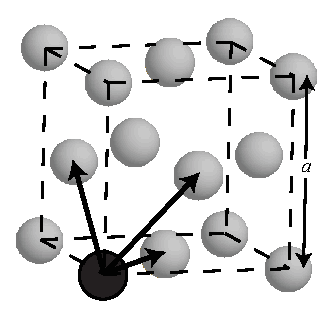
\includegraphics{/home/jason/thesis/thesis/table3-unitcell1.eps} 
& Conventional (four atoms) 
\newline 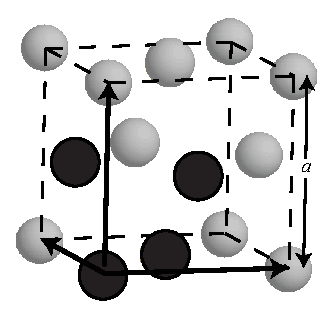
\includegraphics{/home/jason/thesis/thesis/table3-unitcell4.eps}\\ 
\hline
Basis& Face-centered Cubic & Simple Cubic\\ \hline
Lattice Vectors& ($a/2$, $a/2$, 0), \newline ($a/2$, 0, $a/2$), 
\newline (0, $a/2$, $a/2$)& ($a$, 0, 0), \newline (0, $a$, 0), 
\newline (0, 0, $a$)\\ \hline
Brillouin Zone& Truncated Octahedron \newline 
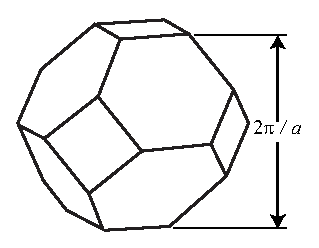
\includegraphics{/home/jason/thesis/thesis/table3-bz1.eps} & Cube \newline 
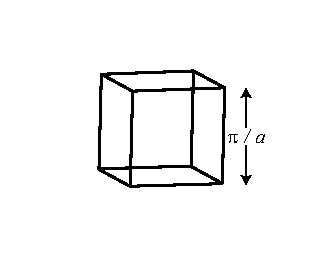
\includegraphics{/home/jason/thesis/thesis/table3-bz4.eps}\\ \hline
Number of \newline Wave Vectors& $N$ & $N/4$\\ \hline
Polarizations/\newline Wave Vector& 3 & 12\\ \hline
\hline
\end{tabular}
\end{center}
\caption{The unit cell for a face-centered cubic crystal can be chosen 
in different ways.}
\label{T-unitcell}
\end{table}
\renewcommand{\baselinestretch}{2.0}
%--------------------------------------------------------------------------

\clearpage

The selection of the unit cell sets the shape of the Brillouin zone and 
the points that will be resolved inside it (i.e., the allowed wave 
vectors, $\pmb{\kappa}$). For a simulation cell with $N$ atoms, there 
are $3N$ normal modes. If the unit cell has one atom, there will be $N$ 
allowed wave vectors, each with three polarizations (i.e., dispersion 
branches, which we will denote by $\nu$). For a four-atom unit cell, 
there will be $N/4$ allowed wave vectors, each with 12 polarizations. 
In general, the choice of an $n$-atom unit cell will lead to $N/n$ 
allowed wave vectors, each with 3$n$ polarizations. As such, there are 
always $3N$ normal modes.

%--------------------------------------------------------------------------
\subsection{\label{A:symmetry}Crystal Symmetries (WORK)}
%--------------------------------------------------------------------------

Symmetry operations define the properties of a crystal. 
This applies to any vector or tensor property of the crystal. The 
symmetries do not depend on the unit cell represenation, although 
conventional unit cells may have additional symmetries compared 
to the primitive unit cells which is due to the redundant information of 
using a conventional cell. 

Ab initio codes such as abinit and quantum espresso also print the 
symmetry operations information. The 
\href{http://spglib.sourceforge.net/}{spglib} 
package contains a library of routines for utilizing the 
symmetry operations of.

Contact Ankit Jain for more information on symmetry operations 
and their application to thermal transport calculations. 

For the crystalline systems studied in Section , the wavevectors 
are averaged over according to their symmetries, 
which reduces the list of wavevectors to the first octant of the 
cubic BZ.\cite{mcgaughey_phonon_2004} This reduction is equivalent 
to applying roations of the 
\href{http://en.wikipedia.org/wiki/Rotation_group_SO(3)}
{SO(3) Group}, or the group of 90 degree rotations in Euclidean 
(3-dimensional) space. 
Any succesive combination of 90 degree roations is also a symmetry 
operation. This property leads to the identity
\begin{equation}\label{EQ:kpt_sym}
 \begin{split}
  \pmb{\kappa} = -\pmb{\kappa},
 \end{split}
\end{equation}
which is the application of two 90 degree rotations, and is a 
\href{http://en.wikipedia.org/wiki/Parity_(physics)#Odd}
{general property of any crystal}. 

\href{https://github.com/jasonlarkin/disorder/blob/master/matlab/issym.m}
{Here is a matlab function} which compares two vectors 
and checks if they are related by any number of orthogonal 
rotations.

For the LJ argon example, further reduction  of the wavectors is 
possible by using all symmetry 
\href{http://spglib.sourceforge.net/#rotation}{rotation operations} 
of the 
\href{http://www.wolframalpha.com/input/?i=face-centered+cubic}
{face centered cubic lattice}. Additional 
\href{http://en.wikipedia.org/wiki/Translational_symmetry}
{translational symmetry operations} may exist. 
For example, for the cubic conventional cell of LJ argon, translational 
symmetries ensure that all four atoms in the unit cell are 
equivalent. Thus, the conventional cell has more total 
symmetries (rotational plus translational) than the primitive cell, 
which is due to the redundant information contained within it. Similar 
to conventional unit cells, crystalline supercells also have a larger 
number of translational symmetries.

%--------------------------------------------------------------------------
\subsection{\label{A:unitcell}Primitive, Conventional, and Supercell 
Representations using Normal Mode Decomposition (WORK)}
%--------------------------------------------------------------------------

Having described the normal mode decomposition theoretical approach and 
computational methodology in Sections \ref{S-NMDformulation} and 
\ref{S-workflow}, we now carry out a case study on a LJ crystal at a 
dimensionless temperature of 0.0827 (corresponding to an argon 
temperature of 10 K). While this temperature is low (the LJ argon Debye 
temperature is around 85 K), it will allow for a clean demonstration of 
the technique. The LJ interatomic potential is computationally inexpensive 
and is thus ideal for use in code development and testing. All results 
will be presented in dimensionless LJ units \cite{ashcroft_solid_1976}. 
The zero pressure lattice constant is 1.556 (Ref. 
\citenum{mcgaughey_phonon_2004}) 
and the potential energy is cutoff and shifted at a distance of 2.5.

From the same simulation cell and atomic data, one can perform normal 
mode decomposition on either the primitive or conventional unit cells.
\footnote{The allowed wave vectors are defined by the basis
and the supercell used to perform the MD simulations. For a supercell 
built using the conventional unit cell, as we use, the allowed wave 
vectors can be labeled using either the conventional or primitive unit 
cell description.  For a supercell built using the primitive unit cell, 
however, all wave vectors cannot be labeled using the conventional unit 
cell description.} The [100] and [111] dispersion curves and density of 
states obtained from harmonic lattice dynamics calculations are plotted 
for each unit cell in Figs. \ref{F-dispersion}(a) and (b). While the 
dispersion curves in each direction show similarities, they are 
necessarily different due to the allowed wave vectors and shape of the 
Brillouin zone (see Table \ref{T-unitcell}). The density of states, 
however, are identical, as expected and required. We note that the 
conventional unit cell description leads to what appear to be optical 
modes. In reality, these modes are a result of zone folding and can be 
mapped directly to acoustic modes in the primitive unit cell description.

The MD simulations are run in the $NVE$ ensemble, the dimensionless 
time step is 0.002, and the equations of motion are integrated using 
the velocity Verlet algorithm. The system is equilibrated for $2^{20}$ 
time steps before collecting data every 25 time steps for an additional 
$2^{20}$ time steps. In order to capture system-size effects, cubic 
simulation cells with between 256 and 6912 atoms are considered 
(corresponding to between four and twelve conventional unit cells, $N_0$, 
in each of the $x$, $y$, and $z$ directions). Ten simulations are 
performed with different initial velocities and the autocorrelations 
(or Fourier transforms) are averaged over the initial conditions and 
symmetric wave vectors before fitting the phonon properties.

\vspace{10mm}
%\clearpage

\begin{figure}[t]
\begin{center}
\includegraphics[scale=1]
{/home/jason/Dropbox/book/m_book_lj_disp_dos_vg_prim_novg-2.eps}
\includegraphics[scale=1]
{/home/jason/Dropbox/book/m_book_lj_disp_dos_vg_conv_novg-2.eps}
\caption{\label{F-dispersion} {Dispersion curves and full Brillouin zone 
density of states for a LJ crystal at a dimensionless temperature of 
0.0827. (a) [100] and [111] dispersion curves and density of states 
based on the primitive (i.e., one atom) unit cell. (b) [100] and [111] 
dispersion curves and density of states based on the conventional (i.e., 
four atom) unit cell. The harmonic lattice dynamics calculations are 
performed using a resolution of sixteen wave vectors along the reciprocal 
lattice vectors of the conventional unit cell. The red and blue dots in 
(b) are the modes considered in Fig. \ref{F-bulkfitting}.}}
\end{center}\normalsize
\vspace*{-0mm}
\end{figure}

\vspace{10mm}
\clearpage

The lifetimes predicted from the frequency-domain analysis for the 
primitive and conventional unit cell representations of the $N_0=10$ 
system are plotted in Fig. \ref{F-bulklifetimes}(a). The difference 
between the lifetimes is less than 5\%, which is within the uncertainty 
of the fitting. A $1/\omega^2$ scaling, predicted from theory for 
phonon-phonon scattering at low frequencies \cite{callaway_model_1959}, 
is plotted and is in good agreement with the trend in the data at low 
frequencies. Also plotted is the Ioffe-Regel (IR) limit 
\cite{taraskin_determination_1999},
\begin{eqnarray}
\tau_{IR} = \f{2 \pi}{\omega},
\end{eqnarray}
which corresponds to when the phonon lifetime is equal to its period. 
All the modes in the perfect system have lifetimes well above this limit. 
It is interesting to note that the phonon lifetimes do not decrease 
monotonically with increasing frequency, with a maximum observed near 
$\omega = 18$. Such a maximum is also observed in silicon lifetimes 
obtained from the SW potential \cite{turney_-plane_2010} and from DFT 
calculations \cite{esfarjani_heat_2011}.

\begin{figure}[t]
\begin{center}
\includegraphics[scale=1]
{/home/jason/Dropbox/book/m_book_lj_nmd_prim_conv_compare-2.eps}
\caption{\label{F-bulklifetimes} Lennard-Jones lifetimes from a 
$N_0=10$ system at a temperature of 0.0827 predicted from normal mode 
decomposition analysis on (a) the primitive and conventional unit 
cells, and (b) treating the simulation cell as the unit cell (i.e., 
Gamma-point analysis). All lifetimes extracted from time-domain analysis.}
\end{center}\normalsize
\end{figure}

\clearpage

In performing the normal mode decomposition, one is not limited to the 
primitive or conventional unit cells. As needed for disordered systems 
(see Sections \ref{S-alloy} and \ref{S-amorphous}) one can define the 
simulation cell as the unit cell, such that all normal modes have 
$\pmb{\kappa}=\mathbf{0}$ (i.e., they are all at the Gamma-point).
\footnote{In Gamma-point analysis, all normal modes have zero group 
velocity and it is not possible to predict mean free paths or thermal 
conductivity.} The lifetimes for Gamma-point analysis for the same MD 
data used to generate the lifetimes in Fig.\ref{F-bulklifetimes}(a)   
are plotted in Fig.\ref{F-bulklifetimes}(b). The trends for the 
Gamma-point analysis are the same as for the primitive and conventional 
unit cells. There is more scatter in the Gamma-point data as wave 
vector symmetry averaging is no longer possible.

The phonon properties obtained from normal mode decomposition and 
harmonic lattice dynamics calculations can now be used to predict bulk 
thermal conductivity using Eq.\eqref{E-kBTE}. For classical MD 
simulations the assumption of equipartition of energy is very good and 
we take the volumetric specific heat to be $k_\mathrm{B}/V$ for all 
modes \cite{mcgaughey_quantitative_2004,goicochea_thermal_2010,
larkin_comparison_2012}.

The Gamma point corresponds to bulk translation and therefore does not 
contribute to thermal conductivity. By discretizing the Brillouin zone, 
we assign a volume to the Gamma point. The zero contribution of this 
volume to the thermal conductivity introduces a size effect in the 
prediction. To predict a bulk thermal conductivity, an extrapolation 
procedure is used, whereby $k$ is plotted versus $1/N_o$ and a line is 
fit to the data. The point on this line where $1/N_o=0$ gives the bulk 
thermal conductivity \cite{turney_predicting_2009,esfarjani_heat_2011}. 
This extrapolation 
procedure requires that the low-frequency modes be dominated by
intrinsic scattering (i.e., $\tau \propto \omega^{-2}$) and have a 
similar group velocity \cite{shiomi_thermal_2011,esfarjani_heat_2011}. 
For the LJcrystal, this requirement is satisfied for modest system sizes
($N_0 \ge 6$). The size-dependent and extrapolated thermal conductivities 
are plotted in Fig.\ref{F-bulksizeeffect} for both the primitive and 
conventional unit cells. The Green-Kubo predictions for the same system 
are also plotted and show no size effect, consistent with previous work 
\cite{mcgaughey_quantitative_2004}.

% \begin{figure}[t]
% \begin{center}
% \includegraphics[scale=1.0]
% {/home/jason/Dropbox/book/m_book_cond_extrap_c0-3_boxon.eps}
% \caption{\label{F-bulksizeeffect} Size dependence of thermal conductivity 
% for the LJ crystal at a temperature of 0.0827 from normal mode 
% decomposition and the Green-Kubo method.}
% \end{center}\normalsize
% \vspace*{-0mm}
% \end{figure}

The extrapolated thermal conductivities from the primitive and 
conventional unit cells are $177 \pm 15$ and $176 \pm 14$ W/m-K. 
The Green-Kubo thermal conductivity is $173 \pm 13$ W/m-K. All thermal 
conductivities agree well within their respective uncertainties.

For the perfect LJ crystal, there is no clear advantage of performing 
the analysis in the time or frequency domains or for the primitive or 
conventional unit cells. Challenges may emerge for high thermal 
conductivity materials like silicon or carbon nanotubes, where the 
time-domain decay may not be well described by an exponential and the 
peaks in frequency space get narrow or are not well-fit by a Lorentzian. 
The failure of the fitting for a perfect crystal is an indication that 
the relaxation time approximation may not be appropriate and that care 
should be taken when interpreting the results. In general, new materials 
should be investigated on a case-by-case basis to determine the approach 
that minimizes the uncertainty.

%--------------------------------------------------------------------------
\section{\label{A:NMD XCORR}NMD using Non-Exact Normal Modes}
%--------------------------------------------------------------------------

In Chapter \ref{Chapter:SED}, it was shown how NMD is 
applied to a perfect crystal. In reality, any crystal will have some 
deviation from perfect periodicity, which may be caused by a point defect, 
a dislocation, a grain boundary, or a free surface. In extreme cases, 
these deviations from periodicity will lead to the emergence of modified 
normal modes. For small perturbations, however, it is reasonable to
assume that the frequencies and mode shapes of the normal modes will 
be unchanged and that the effect of the perturbation will be on the 
lifetimes. Under this assumption, one can still project the atomic 
positions and velocities onto the normal modes of the unperturbed system.

While one could perform the NMD by projecting 
the atomic positions and velocities onto the modes of the unperturbed 
system, it is more appropriate to use the virtual crystal approximation 
(Section \ref{S:From VC Gamma}). 
Under the virtual 
crystal approximation, the system is replaced by one where all atoms 
have the same mass, equal to the average of the atomic masses in the 
system of interest. This system will have the same mode shapes as the 
original system, but the frequencies are modified due to the change 
in the average atomic mass.

Results for the time- and frequency domain approaches to NMD 
are shown for two modes for crystalline and alloyed LJ argon in 
Figs. \ref{F-alloyfitting}(a)-(d). These two modes are equivalent to 
those shown in the perfect crystal in 
Figs. \ref{F-dispersion}(b), \ref{F-bulkfitting}(a), and 
\ref{F-bulkfitting}(b). For a concentration, $c$, of 0.05, both peaks 
in the frequency domain are well-formed and a lifetime can be extracted 
by fitting the data to a Lorentzian function. This behavior is typical 
of all modes at a concentration of 0.05. The downward frequency shift 
is related to the increased average atomic mass.

For an alloy concentration of 0.5, the lower frequency mode still has 
a well-formed peak. The higher-frequency mode does not, however, such 
that a lifetime cannot be extracted by fitting to a Lorentzian function. 
Such behavior is typical of the higher frequency modes at high alloy 
concentrations. This change in behavior is also seen in the time domain, 
where the decay of the autocorrelation of the total mode energy is no 
longer a smooth exponential function. This behavior indicates that the 
virtual crystal normal mode is not a good description of the true 
normal mode. Equation \eqref{E:tau_E_xcorr} can be used to approximate a 
lifetime, as shown in Figs. \ref{F-alloyfitting}(c) and 
\ref{F-alloyfitting}(d).

These artifacts observed using NMD method with the virtual crystal 
approximation are not surprising given two considerations: 
(i) the MD simulations 
contain explicit disorder that influences the atomic trajectories, 
and (ii) the VC-normal modes are not the exact normal modes of the 
explicitly-disordered lattice supercells. 
An effective lifetime can be predicted 
using Eq. \eqref{E:tau_E_xcorr} 
because the VC total mode energy autocorrelations 
still decay to zero in a finite time. This result is to be expected 
given that the atomic trajectories contain 
information about the lattice energy, which from general statistical 
physics principles will have exponential relaxation behavior in an 
equilibrium ensemble.
\cite{landau_statistical_1980,srivastava_physics_1990,
rajabpour_thermal_2010} The lifetimes predicted from the VC-NMD method 
are in reasonable agreement with those predicted from the Gamma-NMD 
method, which uses the exact normal modes of the disordered supercell 
(Section \ref{S:From VC Gamma}).  

% For a normal mode of the lattice supercell 
% used for the MD simulations (i.e., a Gamma mode), 
% the total energy autocorrelation is an exponential function  
% with a decay time $\tau\kv$ and the kinetic energy autocorrelation is a 
% exponentially-damped sinusoidal oscillation with frequency 
% $2\omega\kv$ (see Section \ref{S:Subsection_SED_time-domain}). 
% When projecting MD simulations  
% of the explicitly disordered lattice supercells 
% onto the VC normal modes, 
% the energy autocorrelation functions 
% do not always follow these simple functional forms, 
% as shown in Fig. \ref{F:NMD XCORR} for two modes in the LJ alloy at a 
% concentration of 0.5.  
% By calculating the mode kinetic energy in the  
% frequency-domain, $\Phi$,\cite{larkin_comparison_2012} artifacts such as 
% multiple peaks are observed (see main plot).   



% %--------------------------------------------------------------------------
% \begin{figure}
% \begin{center}
% \includegraphics[scale=1.0]
% {/home/jason/disorder/paper/vc/fig10.eps}
% \vspace*{-5mm}
% \end{center}
% \caption{\label{F:NMD XCORR} The normal mode kinetic energy, $\Phi$,  
% of two modes (A and B) at wavevector [0.25 0 0] calculated 
% using VC-NMD for a mass disordered LJ FCC supercell 
% ($N_0=8$ and $c=0.5$) is shown in the main figure. 
% The VC dispersion-predicted peaks are labeled 
% by $\omega_0$. The inset shows the same mode's energy 
% [kinetic ($KE$) and total ($TE$)] autocorrelation functions.  
% Note the additional oscillation effects in the KE and TE autocorrelation 
% functions for Mode B which are due to the two peaks in $\Phi$. 
% A mode lifetime can 
% be extracted unambiguously using the integral of the TE autocorrelation 
% function [Eq. \eqref{EQ:tau_nmd} in Section \ref{S:From VC Gamma}].}
% \end{figure}
% %--------------------------------------------------------------------------

%--------------------------------------------------------------------------
\begin{figure}[t]
\begin{center}
\includegraphics[scale=1]
{/home/jason/Dropbox/book/m_book_lj_disp_dos_vg_prim_novg-2.eps}
\includegraphics[scale=1]
{/home/jason/Dropbox/book/m_book_lj_disp_dos_vg_conv_novg-2.eps}
\caption{\label{F-dispersion} {Dispersion curves and full Brillouin zone 
density of states for a LJ crystal at a temperature of 
10 K. (a) [100] and [111] dispersion curves and density of states 
based on the primitive (i.e., one atom) unit cell. (b) [100] and [111] 
dispersion curves and density of states based on the conventional (i.e., 
four atom) unit cell. The harmonic lattice dynamics calculations are 
performed using a resolution of sixteen wave vectors along the reciprocal 
lattice vectors of the conventional unit cell. The red and blue dots in 
(b) are the modes considered in Fig. \ref{F-bulkfitting}.}}
\end{center}\normalsize
\vspace*{-0mm}
\end{figure}
%--------------------------------------------------------------------------

%--------------------------------------------------------------------------
\begin{figure}
\begin{center}
\includegraphics[scale=1.0]
{/home/jason/Dropbox/book/m_book_lj_nmd_xcorr_compare_c0_c05_c5_sed.eps}
\includegraphics[scale=1.0]
{/home/jason/Dropbox/book/m_book_lj_nmd_xcorr_compare_c5_xcorr.eps}
\end{center}
\caption{\label{F-alloyfitting} 
Virtual crystal (a) frequency-domain 
and (b) time-domain NMD analysis for two modes 
in LJ alloys with concentrations of 0.05 and 0.5. For modes that are 
not well-approximated by the virtual crystal modes, the lifetime can 
be approximated using Eq. \eqref{E:tau_E_xcorr}, as shown in (d).
}
\end{figure}
%--------------------------------------------------------------------------
\vspace{5mm}
\clearpage

%--------------------------------------------------------------------------
\section{\label{A:metastability}Effect of Metastability for 
Amorphous Solids on Normal Mode Decomposition}
%--------------------------------------------------------------------------

Amorphous materials may have many different atomic 
configurations with nearly equivalent potential energies, 
leading to potential metastability during MD simulations 
\cite{buchenau_structural_1988,feldman_numerical_1999,
durandurdu_<i>ab_2002,bernstein_structural_2006,he_heat_2011}. 
This meta-stability can 
cause errors when predicting vibrational lifetimes using NMD, 
which is demonstrated below. 

This case study is performed on an amorphous LJ system with 2048 atoms 
at a temperature of 5 K. 
The amorphous solid is generated by liquefying the 
crystal, instantaneously removing all kinetic energy, and then relaxing 
the structure (i.e., a melt-quench, Sections \ref{S:Calculation} 
and \ref{S:Sample}). 
The MD simulation parameters are the same as for the 
LJ crystal and alloy (Section \ref{S:Calculation}). 
The LJ 
amorphous phase is metastable at this temperature and intermittently 
moves between very similar low-energy states. Evidence for the 
metastability can be found by analyzing the time-histories of the atomic 
displacements. As such, NMD, which requires the 
average atomic positions, will be an approximation.

The time- and frequency-domain approaches to NMD 
are shown for two mode in the amorphous system in 
Figs. \ref{F-amorphousfitting}(a) and \ref{F-amorphousfitting}(b). 
Because the analysis is performed at the Gamma-point, the peaks are 
well formed, but they are not Lorentzian. 
The oscillations in the total energy 
correlation for the low frequency mode is a consequence of the 
metastability of the amorphous phase. As such, the lifetimes are extracted 
by using Eq. \eqref{E:tau_E_xcorr}, as shown in the inset to 
Fig. \ref{F-amorphousfitting}(b). 
The lifetimes for the amorphous system are plotted in 
Fig. \ref{F-amorphouslifetimes}. Compared to the crystal, the lifetimes 
show little frequency dependence and a significant number at low 
frequencies fall below the IR limit [Eq. \eqref{EQ:IR}]. This result 
seems to be a consequence of the metastability, since this behavior 
is not observed for the NMD-predicted lifetimes for a-SiO$_2$ and a-Si 
(Fig. \ref{FIG:Lifetimes}, Section \ref{S:Life}), 
which were both annealed carefully to remove metastability 
(Section \ref{S:Sample}). Annealing the amorphous LJ system at the 
temperature studied does not remove metastability and leads to 
re-crystallization if performed for a long enough time ($>$ 5 ns). 

\begin{figure}[t]
\begin{center}
\includegraphics[scale=0.85]
{/home/jason/Dropbox/book/m_nmd_xcorr_fit_lj_plot-2.eps}
\caption{\label{F-amorphousfitting} (a) Time-domain and (b) frequency 
domain NMD analysis for two modes in an amorphous 
LJ solid at a temperature of 10 K.}
\end{center}\normalsize
\vspace*{-5mm}
\end{figure}

\begin{figure}[h]
\begin{center}
\includegraphics[scale=0.85]
{/home/jason/Dropbox/book/m_lj_nmd_c0_amor_life.eps}
\caption{\label{F-amorphouslifetimes} Lifetimes predicted by normal 
mode decomposition for an amorphous LJ phase at a  
temperature of 5 K. The lifetimes for the crystal at a 
temperature of 10 K are provided for comparison.}
\end{center}\normalsize
\vspace*{-5mm}
\end{figure}

\clearpage

%--------------------------------------------------------------------------
\section{\label{Appendix_A:Finite}Finite Simulation-Size Scaling for 
Thermal Conductivity}
%--------------------------------------------------------------------------

The thermal conductivities predicted by the NMD ($\Phi$), 
$\Phi'$, 
VC-NMD, VC-ALD, and GK methods 
are system size-dependent [i.e., $k = k(N_0)$] for all lattices 
and amorphous materials methods except 
perfect LJ argon from GK\cite{mcgaughey_quantitative_2004} and 
a-SiO$_2$ (Section \ref{S:Bulk}). 
To predict a bulk thermal conductivity, $k_{bulk}$,  
a linear extrapolation procedure is 
used, whereby 
\begin{equation}\label{EQ:k0}
\frac{k(N_0)}{k_{bulk}} = 1 - \frac{c_0}{N_0},
\end{equation}
where $c_0$ is a constant \cite{turney_predicting_2009,
esfarjani_heat_2011,shiomi_thermal_2011,he_thermal_2011}. 
This procedure is necessary because the first 
Brillouin zone is only sampled at a finite number of points for a finite 
simulation size, with no contribution from the volume at its center. To 
predict a bulk thermal conductivity, it is important to sample points 
near the Brillouin zone center, where the modes can have large lifetimes 
and group velocities \cite{turney_predicting_2009,sellan_size_2010}. 

The thermal conductivity 
is predicted for varying system sizes and the bulk thermal conductivity 
is obtained by fitting Eq. \eqref{EQ:k0} to the data. 
For the NMD ($\Phi$), $\Phi'$, VC-NMD, and VC-ALD methods, 
the validity of Eq. \eqref{EQ:k0}  
requires that the low-frequency modes be dominated by 
phonon-phonon scattering (i.e., $\tau\ \propto \omega^{-2}$) and  
follow the Debye approximation 
with respect to the group velocity and DOS 
\cite{shiomi_thermal_2011,esfarjani_heat_2011}. For the LJ 
argon alloys, this requirement is satisfied for modest system sizes 
(for $N_0 = 6$ to $12$).


%--------------------------------------------------------------------------
% \begin{figure}
% \begin{center}
% \includegraphics[angle=0,width=80.0mm]
% {/home/jason/thesis/thesis/appendix/LJ_NMD_SED_COND_2.eps}
% \end{center}
% \caption{\label{F:LJ_COND} Thermal conductivity predictions for LJ argon 
% calculated using phonon lifetimes predicted by $\Phi$ and $\Phi'$. (a) 
% The finite simulation-size scaling extrapolation 
% \cite{turney_predicting_2009,he_thermal_2011} 
% is used to compare the results to bulk predictions made using the 
% Green-Kubo method. (b) The bulk results for $\Phi$ and Green-Kubo are 
% in good agreement temperatures of $20$ and $40$ K with those of other 
% atomistic simulation methods,\cite{turney_predicting_2009} while those 
% from $\Phi'$ differ (see Table \ref{T:cond_table}).}
% \end{figure}
%--------------------------------------------------------------------------
%\clearpage


%--------------------------------------------------------------------------
\section{\label{Appendix:AF}AF Calculations (WORK)}
%--------------------------------------------------------------------------


% https://github.com/jasonlarkin/disorder/blob/master/lj/alloy/af_di_compare_broadening.m

The AF theory suggests a broadening which is larger than the average 
frequency spacing, $\delta_{avg}$. 

The role of energy broadening in MD simulations could be helpful. The 
energy of a given mode is broadened for two reasons: 

1) due to anharmonic interactions.

2) due to disorder (i.e., phonon-defect scattering in alloys, 
diffuson theory). 

The NMD-predicted lifetimes are predicted from MD simulations where 
all scattering mechanisms are present. Based on the comparison 
of NMD- and AF-predicted diffusivities in Fig. , a frequency-dependent 
broadening may be necessary for the AF theory. The role of frequency 
broadening needs further investigation. 

%--------------------------------------------------------------------------
\subsection{\label{Appendix:AF:Physical}Physical Picture}
%--------------------------------------------------------------------------

The AF theory makes the harmonic approximation. Physically, modes 
couple by spatial and energetic (harmonic, elastic scattering) overlap.  
The strength of the overlap is determined by how close the mode 
energies (frequencies) are and how much the eigenvectors spatially overlap. 
The two highest frequency modes of the LJ alloy at a concentration of 
0.5 (see Section , Fig. ) are shown in Fig. . The mode frequencies are 
and . These modes are both highly localized locons, which is indicated 
by the small amount of spatial overlap in the eigenvector components. Only 
the two spatial-dimensional components of the total three 
spatial-dimensional components of the eigenvectors are plotted. The 
three dimensional atomic coordinates are plotted in two dimensions. 

%--------------------------------------------------------------------------
\begin{figure}
\begin{center}
\includegraphics[angle=0,width=80.0mm]
{/home/jason/disorder/lj/alloy/m_eig_3d_plot_lj_alloy_c5_mode11999_12000.eps}
\end{center}
\caption{\label{F:LJ_COND} Spatial components of the eigenvectors of two 
locons. The spatial localization is evident from the small amount of 
spaital overlap of the mode eigenvectors.}
\end{figure}
%--------------------------------------------------------------------------

\clearpage

%--------------------------------------------------------------------------
\subsection{\label{Appendix:AF:Finite}Finite Size Effects}
%--------------------------------------------------------------------------


% Hi Julian,
% 
% No problem about the silence, I have been busy trying to wrap up my thesis and find a job!
% 
% So, here are the issues:
% 
% 1) On the journey back from the most recent trip I was reading though the draft
% manuscript that you sent me & puzzling over the issue of the size / Lorentzian sensitivity
% of the answers.
% 
% Yes, this is kind of a tricky part of the AF method.  It seems like this was never addressed in the 
% main paper, they simply suggest using a broadening equal to the average frequency spacing,\cite{feldman_thermal_1993} 
% which is continued in \cite{feldman_numerical_1999} and \cite{shenogin_thermal_2009}. 
% It turns out that the frequency spacing \delta_{freq} is strongly freq dependent, especially at low frequencies where the modes 
% are sparse. Here is a crude plot for an a-LJ sample:
% 
% https://github.com/jasonlarkin/disorder/blob/master/lj/alloy/af_di_dw_amor.png
% 
% This has different effects depending on the system.  
% 
% For LJ alloys, the k_{AF} is strongly system-size dependent:
% 
% https://github.com/jasonlarkin/disorder/blob/master/lj/alloy/af_k_kmax.png
% 
% This is due to the harmonic approximation used in the AF theory, which leads to a Rayleigh scaling of 
% the low-freq modes, \tau\propto\omega^{-4}. Here is another crude plot, showing the \omega^{-4} scaling 
% predicted
% 
% https://github.com/jasonlarkin/disorder/blob/master/lj/alloy/af_di_all.png
% 
% While a-LJ shows a dependence on the broadening,  (\bra{\delta}=x*\delta_{avg} in this figure). Amorphous LJ is equivalent to a disordered lattice with a large disorder parameter.\cite{beltukov_ioffe-regel_2013}
% 
% 
% The effect on a-Si is more complicated. For broaden = \delta_{avg}, the diffusivities at low frequency 
% have large fluctuations. No definitive scaling can be seen, there seems to be a mix of \omega^{-4} and \omega^{-2} scalings. 
% 
% By increasing the broadening, the low frequency scaling can be tuned to match \omega^{-2} or \omega^{-4}:
% 
% https://github.com/jasonlarkin/disorder/blob/master/si/amor/m_af_si_normand_N0_3.png
% 
% The low-frequecy fluctuations can be smoothed by increasing the broadening over a small range:
% 
% https://github.com/jasonlarkin/disorder/blob/master/si/amor/m_af_si_normand_N0_5.png
% 
% This exaplins why Shenogin et al.'s prediction of k_{AF} = 1.0 W/m-K for a 512 atom system:
% 
% https://github.com/jasonlarkin/disorder/blob/master/si/amor/m_af_feldman_shenogin_fabian.png
% 
% which is due to using a small broadening. 
% 
% 
% 
% 
% 
% 
% 1) I'm not quite clear on is what the final result is for the K_ph contribution that has to be
% added. I realise that this was an early draft since all the cross referencing etc wasn't 
% finished, and so perhaps you have an updated version that might help?
% 
% Ya sorry, that was a pretty early draft.  Here is the one which is just about to be submitted:
% 
% https://github.com/jasonlarkin/disorder/raw/master/paper/mfp/prb_mfp_jl_081613.pdf

%--------------------------------------------------------------------------
% \begin{figure}
% \begin{center}
% \includegraphics[bb=0 0 3cm 3cm]
% {/home/jason/disorder/lj/alloy/af_di_all.png}
% \end{center}
% \caption{\label{F:LJ_COND} Spatial components of the eigenvectors of two 
% locons. The spatial localization is evident from the small amount of 
% spaital overlap of the mode eigenvectors.}
% \end{figure}
% %--------------------------------------------------------------------------
% 
% 
% %--------------------------------------------------------------------------
% \begin{figure}
% \begin{center}
% \includegraphics[bb=0 0 3cm 3cm]
% {/home/jason/disorder/lj/alloy/af_di_dw_0.05.png}
% \includegraphics[bb=0 0 3cm 3cm]
% {/home/jason/disorder/lj/alloy/af_di_dw_amor.png}
% \end{center}
% \caption{\label{F:LJ_COND} Spatial components of the eigenvectors of two 
% locons. The spatial localization is evident from the small amount of 
% spaital overlap of the mode eigenvectors.}
% \end{figure}
% %--------------------------------------------------------------------------
% 
% %--------------------------------------------------------------------------
% \begin{figure}
% \begin{center}
% \includegraphics[bb=0 0 3cm 3cm]
% {/home/jason/disorder/lj/alloy/af_di_kappa(broaden).png}
% \end{center}
% \caption{\label{F:LJ_COND} Spatial components of the eigenvectors of two 
% locons. The spatial localization is evident from the small amount of 
% spaital overlap of the mode eigenvectors.}
% \end{figure}
% %--------------------------------------------------------------------------
% 
% %--------------------------------------------------------------------------
% \begin{figure}
% \begin{center}
% \includegraphics[bb=0 0 3cm 3cm]
% {/home/jason/disorder/lj/alloy/af_k_kmax.png}
% \end{center}
% \caption{\label{F:LJ_COND} Spatial components of the eigenvectors of two 
% locons. The spatial localization is evident from the small amount of 
% spaital overlap of the mode eigenvectors.}
% \end{figure}
%--------------------------------------------------------------------------



%--------------------------------------------------------------------------
\section{\label{Appendix:SF}Spectral Density of Disordered Modes (WORK)}
%--------------------------------------------------------------------------

%--------------------------------------------------------------------------
% \begin{figure}
% \begin{center}
% \includegraphics[bb=0 0 3cm 3cm]
% {/home/jason/disorder/lj/alloy/dsf_alloy_0.5_mode100.png}
% \includegraphics[bb=0 0 3cm 3cm]
% {/home/jason/disorder/lj/alloy/dsf_alloy_0.5_mode3000.png}
% \includegraphics[bb=0 0 3cm 3cm]
% {/home/jason/disorder/lj/alloy/dsf_alloy_0.5_mode4000.png}
% \end{center}
% \caption{\label{F:LJ_COND} Spatial components of the eigenvectors of two 
% locons. The spatial localization is evident from the small amount of 
% spaital overlap of the mode eigenvectors.}
% \end{figure}
%--------------------------------------------------------------------------


%--------------------------------------------------------------------------
\section{\label{Appendix:Accum}Size-effects for Low-frequency Dominated 
Materials (WORK)}
%--------------------------------------------------------------------------

%--------------------------------------------------------------------------
\begin{figure}
\begin{center}
\includegraphics[angle=0,width=80.0mm]
{/home/jason/disorder/si/alloy/m_ald_taud_si_cond_N0_ald_gk_nmd.eps}
\end{center}
\caption{\label{F:LJ_COND} Spatial components of the eigenvectors of two 
locons. The spatial localization is evident from the small amount of 
spaital overlap of the mode eigenvectors.}
\end{figure}
%--------------------------------------------------------------------------

\clearpage

%--------------------------------------------------------------------------
\section{\label{Appendix:Accum}Accumulation Functions in Alloys 
(WORK)}
%--------------------------------------------------------------------------


%--------------------------------------------------------------------------
\begin{figure}
\begin{center}
\includegraphics[angle=0,width=80.0mm]
{/home/jason/disorder/lj/alloy/m_ald_taud_lj_kaccum.eps}
\end{center}
\caption{\label{F:LJ_COND} Spatial components of the eigenvectors of two 
locons. The spatial localization is evident from the small amount of 
spaital overlap of the mode eigenvectors.}
\end{figure}
%--------------------------------------------------------------------------

\clearpage

%--------------------------------------------------------------------------
\begin{figure}
\begin{center}
\includegraphics[angle=0,width=80.0mm]
{/home/jason/disorder/lj/alloy/xcorr_alloy_cum_cond.eps}
\end{center}
\caption{\label{F:LJ_COND} Spatial components of the eigenvectors of two 
locons. The spatial localization is evident from the small amount of 
spaital overlap of the mode eigenvectors.}
\end{figure}
%--------------------------------------------------------------------------

\clearpage

%--------------------------------------------------------------------------
\begin{figure}
\begin{center}
\includegraphics[angle=0,width=80.0mm]
{/home/jason/disorder/si/alloy/m_ald_taud_si_klambda.eps}
\end{center}
\caption{\label{F:LJ_COND} Spatial components of the eigenvectors of two 
locons. The spatial localization is evident from the small amount of 
spaital overlap of the mode eigenvectors.}
\end{figure}
%--------------------------------------------------------------------------

\clearpage

%--------------------------------------------------------------------------
\begin{figure}
\begin{center}
\includegraphics[angle=0,width=80.0mm]
{/home/jason/disorder/si/alloy/m_ald_taud_si_cond_N0_ald_gk_nmd.eps}
\end{center}
\caption{\label{F:LJ_COND} Spatial components of the eigenvectors of two 
locons. The spatial localization is evident from the small amount of 
spaital overlap of the mode eigenvectors.}
\end{figure}
%--------------------------------------------------------------------------

\clearpage



%--------------------------------------------------------------------------
\chapter{\label{Appendix_HPC}
Research using High Performance Computing}
%--------------------------------------------------------------------------

%--------------------------------------------------------------------------
\section{\label{A:Comp_Env}Setting Up Computing Environment}
%--------------------------------------------------------------------------

% %%--------------------------------------------------------------------------
% %\subsection{Suggested Reading}
% %%--------------------------------------------------------------------------
% 
% %The online encyclopedia \href{http://www.wikipedia.org/}{wikipedia} 
% %has become an excellent resource for technical knowledge. 
% 
% %\href{http://en.wikipedia.org/wiki/Statistical_mechanics}
% %{Statistical Mechanics}/
% %\href{http://en.wikipedia.org/wiki/Condensed_matter}
% %{Condensed Matter}
% %\cite{ashcroft_solid_1976,mcquarrie_statistical_2000}
% 
% %\href{http://en.wikipedia.org/wiki/Phonon}
% %{Lattice Dynamics} with focus on the classical, quantum 
% %and thermodynamic properties of phonons.\cite{peierls_,ziman,
% %wallace_thermodynamics_1976,
% %srivastava_1990,dove_lattice_1993} 
% 
% %\href{http://en.wikipedia.org/wiki/Introduction_to_quantum_mechanics}{Introduction to quantum mechanics and quantum chemistry}
% %\cite{griffiths_introduction_1995} 
% %and more 
% %advanced topics on 
% %\href{https://en.wikipedia.org/wiki/Electron_configuration}
% %{Electron Strucutre} and 
% %\href{http://en.wikipedia.org/wiki/Density_functional_theory}
% %{Density Functional Theory}.
% %\cite{martin_electronic_2004} 
% 
% %Analytical methods for 
% %\href{http://en.wikipedia.org/wiki/Ordinary_differential_equations}
% %{ordinary} and 
% %\href{http://en.wikipedia.org/wiki/Partial_differential_equation}
% %{partial differential equations}, 
% %\href{http://en.wikipedia.org/wiki/Fourier_analysis}
% %{fourier} and 
% %\href{http://en.wikipedia.org/wiki/Statistics}
% %{statistical analysis},\cite{mcquarrie_mathematical_2003} 
% %and 
% %\href{http://en.wikipedia.org/wiki/Numerical_analysis}
% %{numerical analysis}.\cite{moin_fundamentals_2010} For example, 
% %the LJ MD code discussed in Section uses a  
% %\href{http://en.wikipedia.org/wiki/Verlet_integration}
% %{verlet integration method}. 

%--------------------------------------------------------------------------
\subsection{\label{A:Comp_Env:OS}Hardware and Operating System Choice}
%--------------------------------------------------------------------------

The choice of computing hardware determines which operating system(s) 
can be used. The three 
main choices for operating system are 
\href{http://en.wikipedia.org/wiki/Microsoft_Windows}{Windows}, 
\href{http://en.wikipedia.org/wiki/Mac_OS}{Apple OS}, and 
\href{http://en.wikipedia.org/wiki/Linux}{Linux}. Each 
operating system has limitations depending on the hardware it 
operates on.   
For example, Apple OS is primarily used on 
\href{http://en.wikipedia.org/wiki/Macintosh}{Apple hardware}.

The Linux operating system is based on unix, which is the  
\href{http://www.youtube.com/watch?v=7XTHdcmjenI}
{world's most widely used software}. 
Linux runs on systems ranging from 
\href{http://www.pcworld.com/article/250899/mobile_linux_its_not_just_android_anymore.html}
{cell phones} to the world's 
\href{http://www.zdnet.com/20-great-years-of-linux-and-supercomputers-7000018681/}
{largest supercomputers}. For personal computing use, the most widely 
used Linux version is \href{http://www.ubuntu.com/}{Ubuntu}.
It is well-documented with a large community-based discussion 
system. Apple OS is an adequate substitute as it is 
\href{https://en.wikipedia.org/wiki/Unix-like}{unix-like}.

There are many options for installing Ubuntu and the instructions 
can be found at 
\href{http://www.ubuntu.com/}{ubuntu.com}.
Ubuntu is certified on 
\href{http://www.ubuntu.com/certification/}
{PC's from many computer companies}. 
One company, \href{https://www.system76.com/}{system 76}, 
builds computers with Ubuntu pre-installed. I used the 
\href{https://www.system76.com/laptops/model/panp9}
{Pangolin Performance} for over a year of my Ph.D.  However, 
I recommend using the most-portable (i.e., lightest) and 
longest-battery life notebook available such as the 
\href{https://help.ubuntu.com/community/SamsungSeries9}
{Samsung Series 9}  
or \href{https://help.ubuntu.com/community/MacBookAir}{Macbook Air}. 
You will typically be using this notebook to access large computing 
clusters remotely, 
so there is a benefit of having portability and long 
battery life over computational power.  

%--------------------------------------------------------------------------
\subsection{\label{A:Comp_Env:Term}
Terminal, Commands, and Environment Variables}
%--------------------------------------------------------------------------

These instructions work best for the Ubuntu operating system, and will work 
well for other versions of Linux. Systems commands are executed by the 
system 
\href{https://help.ubuntu.com/community/UsingTheTerminal}{terminal}. 
The following Linux system commands have been used extensively throughout 
this work: sudo, cd, pwd, ls, export, echo, grep, sed, vi, cat, 
scp, ssh, which, nohup. 
There are many more Linux commands that are useful. More information can 
be obtained simply by google searching, i.e. 
\href{https://www.google.com/search?q=linux+sed}
{google: linux sed} 

\href{http://en.wikipedia.org/wiki/Environment_variable}{Environment variables}, 
such as 
\href{http://en.wikipedia.org/wiki/PATH_(variable)}{PATH}, 
can store the paths to installed programs and files. 
Here is how to determine what PATH is set to:
\begin{lstlisting}
$ echo $PATH
/opt/Datathief:/opt/VESTA-x86_64:/home/jason/phonopy/phonopy-1.1/bin:...
\end{lstlisting}
Permanent changes to environment variables can be made in the user's 
\href{https://www.gnu.org/software/bash/manual/html_node/Bash-Startup-Files.html}
{.bashrc file}, which is typically located in the /home/user/ directory. 
The .bashrc file is a 
\href{http://www.ghacks.net/2009/04/16/linux-tips-view-hidden-files/}{hidden file} 
noted by its name starting with ".". 
Here is an example 
\href{https://gist.github.com/kparrish/6064111}{.bashrc} from 
\href{https://github.com/kparrish}{Kevin Parrish}. 
This file modifies environment variables such as 
\href{https://help.ubuntu.com/community/EnvironmentVariables}{PATH}  
when a bash terminal session is launched. Changes to environment 
variables are made when a new terminal session is started. 

Shell scripts are relatively low-level sets of system commands 
which can manipulate environment variables 
and the Linux operating system. 
\href{http://linuxcommand.org/wss0010.php}{Here is a simple tutorial} 
on writing shell scripts. 
\href{http://docs.python.org/2/library/os.html}
{Running Linux system commands in Python} can be an effective way of 
generating and manipulating many files with one script. Python 
is a more robust language than lower-level shell scripting. 
\href{https://github.com/ntpl/ntpy/blob/master/examples/thesis/run.lammps.py}
{Here is an example} that generates a series of shell scripts used to 
submit jobs on cluster resources (see next section). The Python script 
finds dummy variable names (SHELL$\_$NAME and PROC$\_$NAME) and replaces them 
with a different string. 

%--------------------------------------------------------------------------
\subsection{\label{A:Comp_Env:Remote}Working on Remote Resources}
%--------------------------------------------------------------------------

At some point during research you will need to execute code on remote 
resources that are typically large computing clusters ($> 100$ central 
processing units). 
You will be provided with a terminal session similar to the session 
provided by Ubuntu with most of the same system commands. 
While I recommend 
\href{https://filezilla-project.org/}{Filezilla} 
for handling the transfer of data and files, 
the functionality of Filezilla is contained in several shell 
commands: ssh and scp. 
Files can be transferred using the following command
\begin{lstlisting}
$ scp -r user@gilgamesh.cheme.cmu.edu:/home/user/directory/ ./
\end{lstlisting}
which will place the ``directory'' and its contents into the pwd 
(./) of the local terminal session. 

There are many variants of the operating systems used for remote 
computing clusters, but the differences are usually small. 
During my work I regularly used the 
\href{http://gilgamesh.cheme.cmu.edu/doc/gilgamesh.html}
{gilgamesh} computing cluster maintained by 
\href{https://github.com/jkitchin}{John Kitchin}. 
\href{http://gilgamesh.cheme.cmu.edu/doc/gilgamesh.html}
{Gilgamesh's documentation} is a good resource for learning how to run 
calculations on a computing cluster.

%--------------------------------------------------------------------------
\section{\label{A:Comp_Env:Programs}
Installing, Writing and Executing Programs}
%--------------------------------------------------------------------------

%--------------------------------------------------------------------------
\subsection{\label{A:Comp_Env:Install}Installing Available Packages}
%--------------------------------------------------------------------------

Before writing any of your own code, it is best to use any useful 
code that may already exist. 
Most Linux operating systems have automatic software installation. 
For Ubuntu, program  management is achieved using the 
\href{https://help.ubuntu.com/community/AptGet/Howto}{apt-get} 
system command:

\begin{lstlisting}
$ sudo apt-get install gfortran
[sudo] password for jason: 
Reading package lists... Done
...
\end{lstlisting}
To check that the package has been installed, use:
\begin{lstlisting}
$ which gfortran
/usr/bin/gfortran
\end{lstlisting}
This shows that gfortran program is installed in the /usr/bin/ folder, 
a common location where automatically installed programs are located. 
Because the 
folder /usr/bin is in the PATH environment variable, 
the program gfortran is always available no matter where you are in 
the system terminal. 

To get more information about the gfortran, use:
\begin{lstlisting}
$ ls -l /usr/bin/gfortran
lrwxrwxrwx 1 root root 12 Apr 22 03:44 /usr/bin/gfortran -> gfortran-4.7
\end{lstlisting}
where we see that /usr/bin/gfrotran "points" to gfortran-4.7. 
This is called a 
\href{http://en.wikipedia.org/wiki/Symbolic_link}{symbolic link}.

%--------------------------------------------------------------------------
\subsection{\label{A:Comp_Env:Avail}Available Packages for 
Thermal Transport Modeling}
%--------------------------------------------------------------------------

Available programs represent opportunities to perform research quickly 
and easily. I suggest reading their documentation carefully and trying 
the tutorials and examples, which are typically computationally 
inexpensive. 

Most of the existing packages listed below cannot be installed using 
Ubuntu's apt-get command, although 
\href{http://lammps.sandia.gov/download.html#ubuntu}
{this feature does exist for LAMMPS} and more packages are likely 
to be added in the future. It is important to read the installation 
documentation carefully. It is also helpful to contact any system 
Linux/Unix system administration staff or other researchers who are 
experienced with installing packages. These people can usually be 
found at campus or local computing centers, or in your own 
research group! 

For a first-time user, I recommend trying to install the LAMMPS 
package as it is one of the easiest and most versatile. It has 
standard installation files for systems ranging from your 
personal computer up to a massively-parallel supercomputer. 
Installation instructions can be 
\href{http://lammps.sandia.gov/doc/Section_start.html#start_2}{found here}. 

Here is a partial list of the packages I have found useful 
in this work:

\begin{itemize}
\item \href{http://lammps.sandia.gov/}{LAMMPS}, including the particularly 
useful 
\href{http://lammps.sandia.gov/threads/threads.html}{mailing list} 
and
\href{http://lammps.sandia.gov/doc/Section_python.html}
{python interface}: parallel molecular dynamics using empirical interatomic 
potentials.
\item \href{http://www.stfc.ac.uk/CSE/randd/ccg/software/DL_POLY/25526.aspx}
{DL$\_$POLY}: parallel molecular dynamics using empirical interatomic 
potentials.
\item \href{http://projects.ivec.org/gulp/}{GULP}: harmonic lattice 
dynamics using empirical interatomic potentials. 
\item \href{http://phonopy.sourceforge.net/}{phonopy}: harmonic 
lattice dynamics with interface for $\emph{ab initio}$ package. 
\item \href{http://www.homepages.ucl.ac.uk/~ucfbdxa/phon/}{PHON}: 
harmonic lattice dynamics with interface for $\emph{ab initio}$ package.
\item \href{http://www.abinit.org/}{ABINIT}: $\emph{ab initio}$ package. 
\item \href{http://www.quantum-espresso.org/}{Quantum Espresso}: 
$\emph{ab initio}$ package. 
\item \href{https://www.vasp.at/}{VASP}: $\emph{ab initio}$ package. 
\item \href{http://icmab.cat/leem/siesta/}{SIESTA}: 
$\emph{ab initio}$ package. 
\item \href{http://www.msg.ameslab.gov/gamess/}{GAMESS}: 
$\emph{ab initio}$ package.
\item \href{http://www.cp2k.org/}{CP2K}: 
$\emph{ab initio}$ package.
\item \href{http://www.icams.de/content/departments/ams/madsen/boltztrap.html}{BOLTZTRAP} 
\item \href{http://www.ks.uiuc.edu/Research/vmd/}{VMD} 
(with 
\href{https://sites.google.com/site/akohlmey/software/topotools}
{topotools}): structure and visualization. 
\item \href{http://jp-minerals.org/vesta/en/}{VESTA}: structure and 
visualization. 
\end{itemize}

I recommend trying this 
\href{https://gist.github.com/kparrish/6064159}{install.sh} created by 
\href{http://www.github.com/kparrish}{Kevin Parrish} which installs 
many programs and packages, including LAMMPS for parallel computing 
with 
\href{http://www.open-mpi.org/}{OpenMPI}.

%--------------------------------------------------------------------------
\subsection{\label{A:Comp_Env:Writing}Writing Programs: 
Compiled versus Interpreted}
%--------------------------------------------------------------------------

If no package exists to perform the calculation you are interested in, 
there is a good chance you are doing something interesting! The next 
step is to implement the algorithm for the calculation you want 
to perform. There are two choices for doing this: 
\begin{itemize}
\item Write your own code. 
\item Build off an existing package. 
\end{itemize}

As outlined in the previous 
section, there are many pre-existing packages with many functionalities. 
The many packages that can perform nanoscale transport calculations use 
\href{http://en.wikipedia.org/wiki/Compiled_language}{compiled} and 
\href{http://en.wikipedia.org/wiki/Interpreted_language}{interpreted}  
languages, often with a mixture of the two. 
The most commonly used compiled languages are 
\href{https://en.wikipedia.org/wiki/C\%2B\%2B}{C/C++} 
(e.g., Linux, LAMMPS) 
and 
\href{http://en.wikipedia.org/wiki/Fortran}{Fortran}
(e.g., GULP, Quantum Espresso, VASP). 
Here is a good discussion on 
\href{http://stackoverflow.com/questions/13078736/fortran-vs-c-does-fortran-still-hold-any-advantage-in-numerical-analysis-thes}
{the strengths of C++ versus Fortran}. Here are excellent tutorials 
of programming in  
\href{http://www.youtube.com/watch?v=XFQ9dw3CyDo&list=PL1D10C030FDCE7CE0}
{C++}
and 
\href{http://www.youtube.com/watch?v=YRTEOFMUTzw&list=PL6A8E21D2E86A0155}
{Fortran}. Learning these languages is essential to adding to existing 
packages. 

Interpreted languages allow for fast code development and debugging. 
The two interpreted languages you are likely to use are 
\href{http://en.wikipedia.org/wiki/MATLAB}{Matlab}  
and 
\href{http://en.wikipedia.org/wiki/Python_(programming_language)}{Python}. 
The key to maximizing the potential of interpreted languages is by 
using the built-in ``vector'' functions and operations provided by the 
\href{http://www.mathworks.com/help/matlab/matlab_prog/vectorization.html}
{Matlab}  
and 
\href{http://faculty.washington.edu/rjl/uwamath583s11/sphinx/notes/html/python_vect.html}
{Python}  
programming libraries. 
Matlab has an excellent built-in guide and google searches will typically 
yield useful results. An open-source substitute for Matlab is 
\href{http://www.gnu.org/software/octave/}
{Octave}, which is capable to running most Matlab scripts.

The following three case studies are performed on my local 
\href{http://www.samsung.com/us/computer/series-9-notebooks}
{Samsung series 9 notebook}. The 
specifications of the computer can be accessed by using:
\begin{lstlisting}
$ cat /proc/cpuinfo 
processor	: 0
vendor_id	: GenuineIntel
cpu family	: 6
model		: 58
model name	: Intel(R) Core(TM) i5-3317U CPU @ 1.70GHz
stepping	: 9
microcode	: 0x17
cpu MHz		: 782.000
cache size	: 3072 KB
physical id	: 0
siblings	: 4
core id		: 0
cpu cores	: 2
apicid		: 0
initial apicid	: 0
\end{lstlisting}

%--------------------------------------------------------------------------
\subsubsection{\label{A:coding_lang:case1}Case-study (a): 
Optimizing Compiled Codes}
%--------------------------------------------------------------------------

The first case study is a 
\href{https://github.com/jasonlarkin/disorder/tree/master/md_serial}
{single C code to perform molecular dynamics 
on LJ argon}. The code uses simple subroutines and operates using 
a single (serial) processor. The 
\href{http://www.cplusplus.com/doc/tutorial/arrays/}
{arrays in this code are built statically}. 
Arrays can be created 
\href{http://www.cplusplus.com/doc/tutorial/dynamic/}{dynamically}, 
which allows for the input of systems with varying number of 
atoms. Additionally, 
\href{http://www.cplusplus.com/reference/vector/vector/}{vectors} 
can be created and destroyed dynamically and have some advantages 
over arrays.  

The code is compiled using the 
\href{http://www.gnu.org/}{GNU project's} 
C++ compiler, \href{http://www.cprogramming.com/g++.html}{g++}:
\begin{lstlisting}
$ g++ ArgonMD.cpp -o ArgonMD_O_g++
\end{lstlisting}
The code can be run and the output can be directed using a useful 
shell operation called 
\href{http://www.linfo.org/pipes.html}{piping}, 
which is demonstrated below:
\begin{lstlisting}
$ ArgonMD_O_g++ > ./ArgonMD_O/output.txt
\end{lstlisting}
The code can be compiled using 
\href{http://gcc.gnu.org/onlinedocs/gcc/Optimize-Options.html#Optimize-Options}
{optimization flags, such as -O and -O3}:
\begin{lstlisting}
$ g++ -O3 ArgonMD.cpp -o ArgonMD_O3_g++
\end{lstlisting}
which greatly decreases the run time of this particular code. 
The total run time 
can displayed by using the shell command 
\href{http://linux.about.com/od/commands/l/blcmdl1_grep.htm}{grep},  
which shows for no optimization:
\begin{lstlisting}
$ grep -A 1 "Total Time" ./ArgonMD/output.txt
Total Time: 38.42 (s)
\end{lstlisting}
for -O optimization:
\begin{lstlisting}
$ grep -A 1 "Total Time" ./ArgonMD_O/output.txt
Total Time: 18.06 (s)
\end{lstlisting}
and for -O3 optimization:
\begin{lstlisting}
$ grep -A 1 "Total Time" ./ArgonMD_O3/output.txt
Total Time: 11.74 (s)
\end{lstlisting}
A useful shell command is 
\href{http://www.tuxfiles.org/linuxhelp/vimcheat.html}{vi}, a 
shell-based text editor, which can display the output within 
a shell terminal:
\begin{lstlisting}
$ vi ./ArgonMD/output.txt
0       1       5.61358 2.01864 5.26596
...
\end{lstlisting}

To compare with the above results, the LAMMPS code is compiled in serial 
using no , -O, and -O3 optimizations.  
The results are contained in folders beginning with ``lmp''.  A useful 
shell function is 
\href{http://www.tuxfiles.org/linuxhelp/tabtrick.html}{tab-twice}, 
where tapping the tab key twice 
will display files and folders which begin with the same 
characters:
\begin{lstlisting}
$ grep -A 1 "Loop time" ./lmp
lmp.in.lj~     lmp_serial/    lmp_serial_O/  lmp_serial_O3/
\end{lstlisting}
The tab key can also be used for  
\href{http://en.wikipedia.org/wiki/Command-line_completion}
{command-line completion} to complete directory and file names. The run 
time for no optimization is:
\begin{lstlisting}
$ grep -A 1 "Loop time" ./lmp_serial/log.lammps
Loop time of 0.718188 on 1 procs for 1000 steps with 256 atoms
--
Loop time of 3.4892 on 1 procs for 5000 steps with 256 atoms
\end{lstlisting}
for -O optimization:
\begin{lstlisting}
$ grep -A 1 "Loop time" ./lmp_serial_O/log.lammps
Loop time of 0.19842 on 1 procs for 1000 steps with 256 atoms
--
Loop time of 0.917175 on 1 procs for 5000 steps with 256 atoms
\end{lstlisting}
and for -O3 optimization:
\begin{lstlisting}
$ grep -A 1 "Loop time" ./lmp_serial_O3/log.lammps
Loop time of 0.164066 on 1 procs for 1000 steps with 256 atoms
--
Loop time of 0.786311 on 1 procs for 5000 steps with 256 atoms
\end{lstlisting}

There is a decrease in run time with increasing optimization 
for LAMMPS and my code. However, for every 
optimization the LAMMPS code is approximately an order of 
magnitude faster.  This result is 
due to a several factors, the most important being 
the implementation of 
\href{http://en.wikipedia.org/wiki/Neighbor_list}{neighbor lists} 
as discussed in the 
\href{http://lammps.sandia.gov/doc/neighbor.html}
{LAMMPS documentation}. The interested reader is encouraged to 
investigate the LAMMPS code further for useful C++ coding 
practices. 

%--------------------------------------------------------------------------
\subsubsection{\label{A:coding_lang:case2}
Case-study (b): Computational Cost of Interpreted Code}
%--------------------------------------------------------------------------

With interpreted languages, the traditional programming practice of using 
loops (for/do/while, etc) will slow the code execution.  To illustrate 
this behavior, the case study compares codes to perform harmonic lattice 
dynamics calculations. 
\href{https://github.com/jasonlarkin/disorder/blob/master/matlab/m_lj_ld_prim.m}
{One code is written in Matlab} using mixture of loops 
and vectorized functions, which slows the code execution. The other 
code is written in Fortran (i.e., the GULP package). 

From within a Matlab session in a terminal, the Matlab code can be 
executed as follows:
\begin{lstlisting}
tic
[freq,eigVsorted,velocity] = m_lj_ld_prim(1.5636*[1 1 1],[0.5 0.0 0.0])
toc
Elapsed time is 0.047081 seconds.
\end{lstlisting}
for the 
\href{https://github.com/jasonlarkin/disorder/blob/master/matlab/m_lj_ld_prim.m}
{primitive}, and
\begin{lstlisting}
tic
[freq,eigVsorted,velocity] = m_lj_ld_conv(1.5636*[1 1 1],[0.5 0.0 0.0])
toc
Elapsed time is 0.260508 seconds.
\end{lstlisting}
for the 
\href{https://github.com/jasonlarkin/disorder/blob/master/matlab/m_lj_ld_conv.m}
{conventional} unit cells. Note that the increased run time is not 
proportional to the increased number of atoms in the unit cell (i.e., 
the calculation does not scale linearly). 
Also note that the two codes both use for loops. This usage slows down code 
execution because Matlab is an interpreted language. 

Now we run the same calculation using the Fortran-based GULP package, for 
the 
\href{https://github.com/jasonlarkin/disorder/blob/master/matlab/gulp_disp_lj_prim.gin}
{primitive}:
\begin{lstlisting}
$ grep -A 6 "Timing analysis " gulp_disp_lj_prim.gout
  Timing analysis for GULP :

---------------------------------------------------------------------------
  Task / Subroutine                                          Time (Seconds)
---------------------------------------------------------------------------
---------------------------------------------------------------------------
  Total CPU time                                                  0.0030
\end{lstlisting}
and 
\href{https://github.com/jasonlarkin/disorder/blob/master/matlab/gulp_disp_lj_conv.gin}
{conventional} unit cells:
\begin{lstlisting}
$ grep -A 6 "Timing analysis " gulp_disp_lj_conv.gout
  Timing analysis for GULP :
---------------------------------------------------------------------------
  Task / Subroutine                                          Time (Seconds)
---------------------------------------------------------------------------
---------------------------------------------------------------------------
  Total CPU time                                                  0.0160
\end{lstlisting}

First, the scaling of the calculation is non-linear. Second, the timing for 
both calculations is over an order of magnitude less than the Matlab versions. 
Matlab code can be optimized by using the built in vector operations and 
functions, which is demonstrated in the next section.

%--------------------------------------------------------------------------
\subsubsection{\label{A:coding_lang:case3}
Case-study (c): Optimizing Interpreted Code}
%--------------------------------------------------------------------------

This case study demonstrates that Matlab (or other interpreted languages) 
can be optimized using the built-in vector functions and operations. 
\href{https://github.com/jasonlarkin/disorder/blob/master/matlab/m_af_template.m}
{This Matlab code} performs the AF theory calculations 
on a LJ amorphous phase of 256 atoms. The code can be run from within 
a Matlab terminal using:
\begin{lstlisting}
>> m_af_template
ans =
    1.5075 (s)
\end{lstlisting}
which calls several subroutines, most notably 
\href{https://github.com/jasonlarkin/disorder/blob/master/matlab/m_af_lj.m}{m$\_$af$\_$lj.m}, 
which uses all vectorized functions. 

Comparing this result with the 
\href{https://github.com/jasonlarkin/disorder/blob/master/matlab/gulp/x0_256.gin}
{same calculation in GULP}:
\begin{lstlisting}
$ gulp x0_256
$ grep -A 10 "Timing analysis " x0_256.gout
  Timing analysis for GULP :
---------------------------------------------------------------------------
  Task / Subroutine                                          Time (Seconds)
---------------------------------------------------------------------------
  Calculation of real space energy and derivatives                0.0520
  Calculation of phonons                                         18.5720
  Calculation of scattering                                       0.0000
---------------------------------------------------------------------------
  Total CPU time                                                 19.3920
---------------------------------------------------------------------------
\end{lstlisting}
The relevant subroutine in GULP to compare with the Matlab version is 
thermalconductivity.f90. 
The GULP timing is considerably larger than the Matlab code.  This is 
due to the use of the default unoptimized 
\href{http://www.netlib.org/blas/}{BLAS} and 
\href{http://www.netlib.org/lapack/}{LAPACK} libraries 
for linear algebra that were used to compile GULP. During the installation, 
Matlab optimizes its linear algebra library, resulting 
in improved performance. 
\nomenclature[A]{BLAS}{Basic Linear Algebra Subprograms} 
\nomenclature[A]{LAPACK}{Linear Algebra PACkage} 

% %--------------------------------------------------------------------------
% \subsection{\label{A:coding_lang:Execute}Executing Programs}
% %--------------------------------------------------------------------------
% 
% %--------------------------------------------------------------------------
% \subsubsection{\label{A:coding_lang:Execute:Local}
% Executing Locally: Rapid Development}
% %--------------------------------------------------------------------------
% 
% %--------------------------------------------------------------------------
% \subsubsection{\label{A:coding_lang:Execute:Remote}
% Executing Remotely: Portable Batch Systems}
% %--------------------------------------------------------------------------

%--------------------------------------------------------------------------
\subsection{\label{A:coding_lang:Execute:Scaling}
Scaling Calculations}
%--------------------------------------------------------------------------

The majority of the methods 
used in this work scale poorly with the number of atoms, $N_a^\alpha$, 
with $\alpha >1$. 
The scaling cost for eigenvalue solution is $N_a^3$. 
The cost of performing this calculation for the largest system size,  
$cost_{large}$,  
and every successive system which is half the size of the largest 
is given by the 
\href{http://en.wikipedia.org/wiki/Geometric_series}{geometric series} 
with common ratio $r=1/8$
\begin{equation}\label{EQ:cost_total}
\begin{split}
cost_{total} = cost_{large}\frac{1}{1-r} = 1.143N_{a,large}. 
\end{split}
\end{equation}
It costs a minimal amount ($ \approx 14\%$) to study every system that 
is smaller 
than the largest system considered. Even a linear scaling   
has (with $r=1/2$) a total cost $cost_{total} = 2cost_{large}$. 
As such, I recommend starting calculations with 
the smallest system of interest (i.e., the 
\href{http://meta.tex.stackexchange.com/questions/3300/minimum-working-example-mwe}
{Minimum Working Example} method). 
Journal article draft manuscripts can be 
developed quickly by performing computationally-inexpensive 
calculations first, documenting the results, and then iterating to more 
computationally-expensive calculations. 
This scheme for performing calculations can follow these time-scales 
for calculation costs:
\begin{itemize}
\item 1 second: exploratory work, debugging.  
\item 1 minute/1 hour: testing the scaling of algorithms, precision  
\item 1 day: publication-quality calculations
\item 1 week: publication-quality calculations, but should be limited 
to when necessary. 
\end{itemize}
I have performed 
countless calculations costing around one second, and very few which cost 
more than one week. Publication quality results will typically 
cost between one hour and one week.
\nomenclature[V]{$cost_{total}$}{total computational cost} 

%--------------------------------------------------------------------------


%%--------------------------------------------------------------------------
%\subsection{Importance of Open-Source Code}
%%--------------------------------------------------------------------------

%LAMMPS Mailing List
%http://lammps.sandia.gov/threads/threads.html

%search: 

%lennard (jones)	45
%silicon		125
%nanotube	153
%ger


%Execellent discussion of ensembles and newtonian dynamics
%http://lammps.sandia.gov/threads/msg13979.htmlmanium	2
%silica		79
%carbon		181
%hydrogen	99
%fullerene(C60)	7(12)	
%Pb (lead)	2
%water		541
%copper(cu)	25
%gold		81
%diamond		43

%phase transition	21
%green kubo	18


%Execellent discussion of ensembles and newtonian dynamics
%http://lammps.sandia.gov/threads/msg13979.html

%video of python development tree

%\href{http://www.youtube.com/watch?v=3poNeQHUKrs}
%{google+ history with gource}

%\href{http://www.youtube.com/watch?v=cNBtDstOTmA}
%{python history with gource}

%grand-daddy of them all, 
%\href{http://www.youtube.com/watch?v=pOSqctHH9vY}
%{linux kernel history with gource}

%It is important that results become more open-source.  It's important 
%that our communication becomes open-source. It's important that the 
%entire numerical process be carried out open-source. 


%%--------------------------------------------------------------------------
%\subsection{Redundancy}
%%--------------------------------------------------------------------------
%
%There are 3 different codes (shiomi/esfarjani, broido, ankit) for 
%performing the same basic calculations.
%
%For LD, there is GULP, phonopy, SIESTA, etc.
%
%%--------------------------------------------------------------------------
%\subsection{Code Development}
%%--------------------------------------------------------------------------
%
%took ankit 10 months to re-develop esfarjani code.  
%
%code development time can be drastically reduced using pre-existing code. 
%codes written in a modular fashion can be added to easily.
%
%%--------------------------------------------------------------------------
%\subsection{Experiment Pre-dating Simulation}
%%--------------------------------------------------------------------------
%The ideal goal of simulation is to pre-date experiment.  This has not 
%been achieved yet.  See Fig.
%
%findings for:
%CNT/Graphene
%Si
%Thermoeletric (LUC, alloys, SL, etc)
%Perovskites
%PCM
%
%%--------------------------------------------------------------------------
%\subsection{Experiment Pre-dating Simulation}
%%--------------------------------------------------------------------------
%
%ntpl most cited paper 1-5:
%maradudin, ladd, dove, ziman, 

%--------------------------------------------------------------------------
\section{Preparing Journal Articles and Thesis}
%--------------------------------------------------------------------------

The job of the student is to prepare, submit, and publish 
peer-reviewed journal articles. There are many journals suitable for 
nanoscale transport topics. All of them accept 
\href{http://www.latex-project.org/}{Latex} prepared manuscripts. 
I recommend the Latex editor 
\href{http://kile.sourceforge.net/}{Kile}, while the simple 
\href{https://projects.gnome.org/gedit/}{gedit} works well and comes 
pre-installed with Ubuntu. Here is a 
\href{http://mally.stanford.edu/~sr/computing/latex-example.html}
{simple latex example} and how to generate a 
\href{http://tex.stackexchange.com/questions/1596/how-to-compile-a-latex-document}
{portable document format (PDF)} from the latex document.  

I recommend editing a written research document at least once every week. 
The exchange of such a document with the advisor can be facilitated using 
\href{https://www.dropbox.com/}{Dropbox} or 
\href{https://github.com/}{Github}. 
Github offers advantages over Dropbox, such as version control and a 
\href{https://github.com/ntpl/ntpy/wiki}{built-in online wiki}. 
Such a research document can turn into journal articles, 
which then turn into the thesis.  

To maintain the reference library I 
recommend 
\href{http://www.zotero.org/}{zotero}.  Here is an example 
\href{https://github.com/jasonlarkin/disorder/blob/master/paper/vc/jap/ntpl-032013.bib}
{reference.bib} 
file which is exported automatically by zotero. 
The references are generated from the latex document using 
\href{http://www.bibtex.org/Using/}{bibtex}, which compiles the contents of 
the reference.bib.

\href{https://github.com/jasonlarkin/disorder/blob/master/paper/vc/jap/jap_vc_jl_060413.tex}
{Here is an example} of the latex file 
used to create an article published from this work. 
This file uses 
\href{http://publish.aps.org/revtex}{revtex}, 
which is an article class used by $\emph{Physical Review}$, 
$\emph{Journal of Applied Physics}$, and others.
\href{https://github.com/robsimmons/cmu-thesis}
{Here is a Carnegie Mellon thesis template}, 
which was used to create 
\href{https://github.com/jasonlarkin/thesis/tree/master/thesis}
{this thesis document}.

% \href{http://web.science.mq.edu.au/~rdale/resources/writingnotes/latexstruct.html}
% {Article on structuring large documents.}
% %--------------------------------------------------------------------------
% \subsection{Producing Figures}
% %--------------------------------------------------------------------------
% 
% Python has a plotting module, \href{http://matplotlib.org/}{matplotlib}, 
% which has \href{http://matplotlib.org/examples/index.html}{many examples}. 
% Here is a \href{https://gist.github.com/kparrish/6101681}{simple example 
% demonstrating how to generate and save data, load that data, and plot.} 
% 
% 
% \href{https://github.com/ntpl/ntpy/tree/master/examples/thesis}
% {Here is a simple example demonstrating how to }

%--------------------------------------------------------------------------
\section{Technical Advice}
%--------------------------------------------------------------------------

In addition to your advisor and close mentors, 
I recommend communicating with experts in the field as much as 
possible (without being annoying).  How often to 
communicate depends on the situation. 
It is best to let the expert dictate the pace of the conversation. 
Here is a list of experts I used as resources for this work. They 
will typically answer emails within 24-48 hours:

\begin{itemize}
\item \href{http://www.engineering.pitt.edu/WissamAlSaidi/}
{Wissam Al-Saidi}
\item \href{http://www2.mpip-mainz.mpg.de/~donadio/tnt/People.html}
{Davide Donadio}
\item \href{http://johncduda.com/}
{John Duda}
\item \href{http://mech.rutgers.edu/content/keivan-esfarjani}
{Keivan Esfarjani}
\item \href{mailto:joseph.feldman.ctr@nrl.navy.mil}
{Joseph Feldman}
\item \href{http://chemistry.curtin.edu.au/people/academic.cfm/J.Gale}
{Julian Gale}, \href{http://projects.ivec.org/gulp/news.html}
{(GULP author)}
\item \href{http://quasiamore.mit.edu/pmwiki.php?n=Main.JivteshGarg}
{Jivtesh Garg}
\item \href{https://github.com/ankitjainmeiitk}
{Ankit Jain}
\item \href{https://github.com/jkitchin}
{John Kitchin}
\item Axel Kolhmeyer via the 
\href{http://lammps.sandia.gov/threads/threads.html}{LAMMPS mailing list} 
and \href{akohlmey@gmail.com}{email}
\item \href{http://jasonlarkin.github.io}{Jason Larkin}
\item \href{http://www.cmu.edu/me/malen/Lab_Website/People.html}
{Jon Malen}
\item \href{http://www.ce.cmu.edu/people/faculty/maloney.html}
{Craig Maloney}
\item \href{http://ntpl.me.cmu.edu/people.html}
{Alan McGaughey}
\item \href{http://www.pmc.umontreal.ca/~mousseau/site_an/}
{Normand Mousseau}
\item Steve Plimpton via the 
\href{http://lammps.sandia.gov/threads/threads.html}{LAMMPS mailing list} 
\item \href{http://www.chem.polimi.it/people/faculty/guido-raos/}
{Guido Raos}
\item \href{http://utexas.academia.edu/DanSellan}
{Dan Sellan}
\item \href{http://www.phonon.t.u-tokyo.ac.jp/}
{Junchiro Shiomi}
\item \href{http://atztogo.users.sourceforge.net/}{Atz Togo}, creator of 
\href{http://phonopy.sourceforge.net/}{phonopy}
\end{itemize}

%D) References – >see discussion in Section 6.9
%E) Appendices – each appendix should have a title and be listed in the 
% Table of Contents

%6.4 Page Numbering
%Each page in a thesis or dissertation should be assigned a number. The 
% following plan of page numbering generally is accepted:
%A) For Preliminaries – use small Roman numerals (i, ii, iii, iv, etc.). 
% The numbering begins with ii; the title page counts as page i, but the 
% number does not appear.
%B) For Remainder of Thesis or Dissertation – including the text, 
%illustrations, appendices, and bibliography, use Arabic numerals 
% (1, 2, 3, 4, etc.). Each page must be numbered. Try to avoid use of 
% letter suffixes such as 10a, 10b. The numbering begins with 1 and runs 
% consecutively to the end of the dissertation.
%C) For More Than One Volume – each volume should contain a title page 
% duplicating the title page of the first volume. If the volumes are 
% separate entities, identify them further as Volume I, II, etc. In any 
% case, the numbering may follow consecutively from one volume to another, 
% or begin with Arabic 1 at each new title page.

%6.5 Footnotes
%If footnotes are needed, they should be placed at the bottom of the page 
% below a 1.5 inch underscore (starting at the left border). The first 
% line of each footnote should be indented 0.5 inches and identified by a 
% raised numeral corresponding to that used in the test. Footnotes should 
% be numbered consecutively throughout each chapter.


%F) Table of Contents – with page references
% %--------------------------------------------------------------------------
%\listoffigures
% %G) List of Tables – with titles and page references
%\listoftables
% %H) List of Figures and Illustrations – with titles and page references.
% %--------------------------------------------------------------------------


\backmatter

%\renewcommand{\baselinestretch}{1.0}\normalsize

% By default \bibsection is \chapter*, but we really want this to show
% up in the table of contents and pdf bookmarks.
\renewcommand{\bibsection}{\chapter{\bibname}}
%\newcommand{\bibpreamble}{This text goes between the ``Bibliography''
%  header and the actual list of references}
\bibliographystyle{unsrt}
\bibliography{/home/jason/Dropbox/ntpl-paper/ntpl-072613} %your bib file
%--------------------------------------------------------------------------
\end{document}
